% Time-stamp: <2020-12-03 21:37:38 Romain>
% LateX template 
% August 2020, Romain Lafarguette, rlafarguette@imf.org

%% ---------------------------------------------------------------------------
%% Preamble: Packages and Setup
%% ---------------------------------------------------------------------------
% Document class and font
\documentclass[11pt]{article}

% Language
\usepackage[english]{babel}

% Layout
%\usepackage[margin=1in]{geometry}
\usepackage[DIV=12]{typearea} % Page layout & margin set-up
\usepackage{setspace} % Linespread
\onehalfspacing % x 1,5 spacing

% Font and encoding
\usepackage[utf8]{inputenc} % For input
\usepackage[T1]{fontenc} % For outut
\usepackage{lmodern} % Standard LateX font
\usepackage[babel=true]{microtype}  % "Subliminal refinements towards typographical perfection"
\microtypesetup{final, tracking=true, kerning=true, spacing=true}

% Graphics
\usepackage{graphicx} % Insert graphics
\graphicspath{{../output/}} % Relative paths for graphics

% Tables
\usepackage{booktabs, rotating, multirow, pdflscape} % Tabular rules and other macros

% Floats, captions and footnotes
\usepackage{float, caption, capt-of}
\captionsetup{font=large}
\newcommand{\source}[1]{\caption*{\raggedright \small {#1} \normalsize}} % Source of a chart, left aligned


% Table of contents
\usepackage[titles]{tocloft}
\renewcommand{\cftsecleader}{\cftdotfill{\cftdotsep}} % Dot every items

% Mathematics 
\usepackage{amsmath, amsthm, amssymb, mathtools, bm} % American Mathematical Society macros 

% Subfiles and separate compilations
%\usepackage{subfiles}

% Manage authors and affiliations
\usepackage{authblk} % Properly align institutions name in the title page

% References and hyper references 
\usepackage{url} % Insert url
\usepackage{natbib} % Year-name format
\usepackage{color}  % Color package
\definecolor{darkblue}{rgb}{0,0,0.44} % Customized color for external hyper references
\definecolor{burgundy}{rgb}{0.5, 0.0, 0.13} % Customized color for internal hyper references

% Hyperlinks in pdf
\usepackage[pdftex]{thumbpdf} % Thumbnails
\usepackage[%
    bookmarks=true,   % bookmarks
    bookmarksnumbered=false,
    pdfpagemode=, % bookmark closed at the opening
    pdfstartview=FitH, % all the heigth
    pdfpagelayout=SinglePage, % perpage view
    colorlinks=true, % Coloured links
    breaklinks=true, % new line for too long links
    urlcolor= darkblue, % external links color
    citecolor=darkblue, % bibliography citations
    linkcolor=burgundy, % Internal links color
    pdfborder={0 0 0}   % No borders
    ]{hyperref} % Extensive support for hypertext in LaTeX

\hypersetup{% PDF metadata
  pdftitle = {Foreign Exchange Intervention Rule for Central Banks: A Risk-Based Framework},
  pdfauthor = {Lafarguette and Veyrune},
  pdfkeywords = {Foreign Exchange Intervention Rule for Central Banks: A Risk-Based Framework},
  pdfsubject = {Finance, Financial Economics},
  pdfcreator = {Lafarguette and Veyrune},
  pdfproducer = {Lafarguette and Veyrune},
  pdfpagemode = {UseOutlines}, % When opening pdf. UseOutlines, FullScreen, etc. 
  pdfstartview = {Fit}}

% Footnote without marker, for the title
\newcommand\blfootnote[1]{%
  \begingroup
  \renewcommand\thefootnote{}\footnote{#1}%
  \addtocounter{footnote}{-1}%
  \endgroup
}

% A few macros: environments
\newenvironment{wideitemize}{\itemize\addtolength{\itemsep}{10pt}}{\enditemize}
\newenvironment{wideenumerate}{\enumerate\addtolength{\itemsep}{10pt}}{\endenumerate}


%% ---------------------------------------------------------------------------
%% Title, authors and affiliations
%% ---------------------------------------------------------------------------
\title{\textbf{Foreign Exchange Intervention Rule for Central Banks:
A Risk-Based Framework}}

\author{Romain Lafarguette}
\author{Romain Veyrune}
\affil{International Monetary Fund} 
\date{December 2020}

%% ---------------------------------------------------------------------------
%% Begin the document
%% ---------------------------------------------------------------------------
\begin{document}

\maketitle      \blfootnote{Contacts:      \url{rlafarguette@imf.org}      and
\url{rveyrune@imf.org}. Corresponding author: \url{rlafarguette@imf.org}. Both
at the Monetary and Capital Markets  Department of the IMF.  The authors thank
Suman Basu, Dimitris Drakopoulos, Kelly Eckhold, Chris Erceg, Andres Gonzales,
Simon Gray, Darryl King, Vladimir  Klyuev, Jorge Kriljenko, Istvan Mak, Thomas
McGregor, Stephen  Mulema, Umang Rawat,  Olga Stankova, and Kevin  Wiseman for
their  comments and  insights.  Karen  Lee provided  research assistance.  The
public  data and  Python codes  to  replicate the  results of  this paper  are
available  at \url{https://romainlafarguette.github.io/software/}.   The views
expressed  in  IMF  Working  Papers  are  those of  the  authors  and  do  not
necessarily  represent the  views  of the  IMF, its  Executive  Board, or  IMF
management.}

%% ---------------------------------------------------------------------------
%% Abstract
%% ---------------------------------------------------------------------------

\begin{abstract} This  paper presents  a new rule  for central  banks’ foreign
exchange (FX) interventions, using the concept of Value at Risk (VaR). The VaR
rule is  used to design an  intervention policy that consistently  transfers a
given share of exchange rate risk from  the market to the central bank balance
sheet, depending  on the economy exposure  to exchange rate risk.  A VaR-based
intervention  rule is  desirable for  countries under  floating exchange  rate
arrangements,  where central  banks intervene  in  the FX  market to  preserve
financial stability. This approach is  consistent with the price and financial
stability mandates of  many central banks, including  inflation targeters. The
VaR  rule has  other appealing  features  for central  banks, including  being
forward  looking and  budget neutral  over the  medium term.  The VaR  rule is
back-tested on Banco Mexico’s publicly available FX interventions data between
2008  and  2016,  both  with  and  without  a  preannounced  fixed  volatility
threshold.\\
\end{abstract}
\bigskip

\noindent \textbf{Keywords:} Foreign Exchange Interventions, Value at Risk, Exchange Rate at Risk, GARCH 

\medskip

\noindent \textbf{JEL classification:} E58 (Central Banks and Their Policies), F31 (Foreign Exchange), G17 (Financial Forecasting and Simulations)

%% ---------------------------------------------------------------------------
%% Suppress page number on title page 
%% ---------------------------------------------------------------------------
\thispagestyle{empty} 
\newpage
\pagenumbering{arabic}


%% ---------------------------------------------------------------------------
%% Table of contents, list of figures and tables
%% ---------------------------------------------------------------------------

\begin{NoHyper}  
\tableofcontents
%\addtocontents{toc}{~\hfill\textbf{Page}\par}
\thispagestyle{empty} 

\listoftables
%\addtocontents{lof}{~\hfill\textbf{Page}\par}
\thispagestyle{empty} 

\newpage
\listoffigures

% \addtocontents{lot}{~\hfill\textbf{Page}\par}
\thispagestyle{empty} 
\end{NoHyper}  

%% ---------------------------------------------------------------------------
%% Introduction
%% ---------------------------------------------------------------------------
\newpage
\pagenumbering{arabic} % Start officially the numbering

\section{Introduction}
\label{sec:introduction}

The 2018 IMF  Annual Report on Exchange Arrangement  and Exchange Restrictions
classified 65  exchange arrangements as  either floating or free  floating, of
which 38 implemented  inflation targeting.  In those  arrangements, the supply
and demand  in the foreign  exchange (FX)  market determine the  exchange rate
with no predictable path.  As a result,  the exchange rate risk is not managed
by the  authorities and  remains fully  with the  private sector,  despite the
financial stability risk  that it entails. As hinted by  the breakdown between
floating  and “free”  floating, not  all  central banks  are comfortable  with
ruling out participation in the FX market. Even those with a strong commitment
to floating, for  example, Chile, Mexico, and Norway, did  intervene in the FX
market   in   cases   of   exceptional    stress,   such   as   the   COVID-19
pandemic.\footnote{See, for example,\\
\url{https://www.fx-markets.com/foreign-exchange/4624581/chile-launches-biggest-fx-intervention-in-20-years},\\
\url{https://www.wsj.com/articles/norwegian-krone-soars-amid-signs-of-central-bank-intervention-11585068173}}\\

Typical FX intervention objectives in a floating exchange rate arrangement are
variants of  preserving market  functioning, for example,  smoothing excessive
exchange  rate  volatility and  addressing  disorderly  market conditions,  or
correcting exchange rate misalignment. The  literature adds objectives such as
an adequate stock  of reserves, external competitiveness,  and price stability
(\cite{patel2019},  \cite{chamon2019}). These  all circle  back to  notions of
market  stability  (having enough  foreign  reserves  to intervene  later)  or
exchange rate  equilibrium (external and  price stability), both of  which are
underpinned by the notion of macrofinancial risk to the economy.\\

The main  contribution of this  paper is to  look at intervention  through the
prism of risk. Each economy presents  to a different extent unhedged exposures
to  exchange rate  risk. Unhedged  exposures  include any  direct or  indirect
exposition to  exchange rate risk  by any economic agents.  They fundamentally
depend on structural features of the  economies, chiefly their size and degree
of openness. The degree of resilience  to foreign exchange risk―that is, large
swings in the  exchange rate―that the economy can  absorb varies substantially
across countries.  As interventions  in the FX  spot market  transfer exchange
rate  risk off  the  market, FX  interventions  can be  desirable  even for  a
floating exchange  rate regime,  as maintaining orderly  conditions on  the FX
market is part of a broad financial stability mandate.\\

Central banks usually  keep a fair degree of opacity  about their intervention
triggers, which  makes it difficult to  determine how much exchange  rate risk
they   consider  the   market   could  manage   on  its   own   and  when   to
intervene. However,  it could be  inferred from actual intervention  if enough
data on  interventions are published.  Other  central banks, such as  those in
Colombia,   Guatemala,  and   Mexico,  use   transparent  intervention   rules
\citep{chamon2019} that reveal, at least partially, their risk tolerance.\\

This  paper proposes  an  empirical  methodology based  on  Value  at Risk  to
determine  the  trigger of  an  FX  intervention  rule  anchored to  the  risk
tolerance of the central bank (the VaR rule) that absorbs a constant amount of
exchange rate risk and leaves the rest in the market. This risk-based strategy
is beneficial both from a financial stability angle and because of its support
of the development of the FX risk hedging market. This methodology can also be
used  to  reverse  engineer  central  banks' risk  tolerance  based  on  their
intervention in the FX spot market.\\

There are important conceptual caveats to  mention. Our paper does not explore
the efficiency of FX interventions, as  we use a simple reduced-form framework
without causal identification.  The paper  focuses on the timing (the trigger)
for intervention  and not  on the optimal  intervention amount.   Further work
could explore these issues.\\

This paper relates to the  rule-versus-discretion literature. The paper argues
that  the VaR  rule offers  many of  the benefits  attached to  the rule-based
approach  while  minimizing common  pitfalls  of  rules.   In this  sense,  it
contributes to  constant efforts  of central  banks to  improve the  design of
policy rules  \citep{taylor2017} in the  domain of exchange rate  policy.  The
most remarkable advantage  of the VaR-based intervention is that  it keeps the
risk  transfers constant,  while it  would increase  or decrease,  possibility
without   limit,  with   exchange  rate   volatility  under   fixed-volatility
triggers.\\

The  empirical methodology  is applied  to the  case of  Mexico. The  peso has
floated for a long period in one  of the most liquid FX markets among emerging
economies.  In  addition,  Banco   Mexico's  (BM)  website  provides  detailed
intervention data since 2008. Banco Mexico also implemented interventions both
with a  minimum bid rate (that  is, a preannounced fixed  volatility rule) and
without  a  minimum  bid  rate,   providing  a  diversity  of  experiences  in
intervention  strategy.  Our  paper  focuses  on  only  one  dimension  of  FX
interventions: preventing  excessive volatility  on the FX  market benchmarked
against a risk-based metric. Other relevant  reasons and motives may well have
been factored into BM intervention without a minimum price.\\

The rest  of the paper  is organized as follows:  Section \ref{sec:literature}
presents  a  brief  literature  review.   Section  \ref{sec:var-interventions}
explains the concept of the exchange rate at risk and the formalization of the
FX  intervention  rule.   Section \ref{sec:empirical-framework}  presents  the
empirical     framework    based     on     a     GARCH    model.      Section
\ref{sec:operational-framework} provides the operational framework for central
banks    using   the    model    for   their    FX   interventions.    Section
\ref{sec:mexico-case}  back-tests the  model  on Mexico  public data.  Section
\ref{sec:conclusion} concludes.\\

%% ---------------------------------------------------------------------------
%% Literature Review
%% ---------------------------------------------------------------------------
\section{Literature Review}
\label{sec:literature}

The literature on policy rules mainly focuses on the monetary policy decision.
The  debate is  essentially whether  the  monetary policy  decision should  be
guided by a  pre-established reaction function (the rule)  or by policymakers’
expert judgment (discretion).  The reasoning is that rules reduce  the cost of
disinflation  policy  if the  monetary  authorities  have not  established  an
inflation aversion reputation by curbing  an inflation expectation of rational
economic agents \citep{kydland1977}.  Once  a reputation has been established,
the  rule  may  not  be  superior   to  discretion  based  on  sound  judgment
\citep{barro1983}.\\

While less  explored in the literature,  the same arguments could  apply to FX
intervention  rules. They  can  likely  signal the  commitment  to a  floating
exchange rate (within boundaries) and convince rational economic agents (which
may challenge  the central bank  commitment to  float) that the  exchange rate
will experience at least a certain degree of volatility. In addition, FX rules
serve to anchor market expectations \citep{montoro2013} and  to provide
some sense of safety to the market, thereby contributing to its stability.\\

More  generally,  central banks’  commitment  can  be  used to  steer  agents’
behavior. For example, \cite{krugman1991} shows that a commitment to intervene
as the  exchange rate leaves  a target zone causes  change in the  behavior of
economic  agents,  even  when  there   is  no  explicit  intervention.   Also,
\cite{fanelli2020} show  that commitment to future  interventions is necessary
to have an impact on exchange rates today.  Finally, \cite{basu2018} show that
commitment  has additional  benefits over  discretion when  there are  capital
outflows and FX reserves may run out.\\

An important  aspect to consider for  FX interventions is the  source of shock
that the central bank would like  to mitigate. In micro-founded optimal policy
frameworks, the rationale for FX interventions depends on the shock generating
the exchange rate  movement. For example, in \cite{basu2020}, exchange
rate movements  owing to permanent  real shocks―for example,  productivity and
commodity  prices,  and fundamental  changes  in  world interest  rates―should
generally be accommodated unless they trigger financial constraints. Financial
stability depends both  on cyclical (exchange rate  volatility) and structural
factors such that domestic FX hedging,  not just the exchange rate volatility,
could motivate  the central banks  to smooth movements associated  with higher
uncovered interested  rate parity (UIP)  premia. Therefore, according  to this
literature, only  those exchange  rate movements associated  with identifiable
global financial shocks and growing bid-ask  spreads should be included in the
rule,  while movements  arising  from  commodity price  shocks  should not  be
included. However, in  practice, the diagnosis of the  shock requires judgment
(\cite{basu2020}, \cite{cavallino2019}), and  identifying in  real time  the
source of the shock is often not possible. Therefore, the FX intervention rule
we present here has a somewhat narrow focus. The rationale for the VaR rule is
to preserve orderly market conditions by preventing excess volatility and tail
risks to  materialize, irrespective of  their source. One important  aspect is
that  any  source  of  shocks  could  potentially  degenerate  into  financial
stability risks, as long as it creates risks to unhedged exposure. This is the
reason we do  not identify the source  of the shock in this  paper, which also
has benefits in terms of implementation.\\

In  this  paper, an  intervention  is  deemed rule  based  when  it reacts  to
predetermined parameters to deliver predictable responses. The most used rules
are  based  on fixed-volatility  triggers  such  as day-to-day  exchange  rate
change, for  example, 2  percent depreciation from  the previous  day exchange
rate close.   The rule can  be disclosed or kept  secret by the  central bank,
although,   in   the   latter   case,   it   may   become   transparent   with
experience. \cite{patel2019} surveyed 21 emerging market central banks and six
out  the   21  regularly  use   an  intervention   rule,  while  four   do  so
occasionally.\\

Some studied the  efficiency of FX rules and usually  find them less efficient
than discretion. However,  in some cases, the understanding  of rules includes
tactics such as  "leaning against the wind," that is,  delaying the adjustment
of the  exchange rate,  which would  not be  considered a  rule in  this paper
\citep{chutasripanich2015}. In other cases, it  involves central banks with an
already  established  preference  for   floating,  for  which  the  literature
indicates that the  rule may not be superior  to discretion \citep{fatum2005}.
While   country-specific   empirical    work   on   rule-based   interventions
(fixed-volatility  triggers) was  performed for  Canada \citep{fatum2005}  and
Columbia  \citep{kuersteiner2018},  none  was  completed for  Mexico,  to  our
knowledge.\\

The concept of VaR, as formalized in \cite{jorion2007}, is frequently used for
financial applications, for managing  risk exposure, for portfolio allocation,
and so  on. \cite{alexander2009}  provides a comprehensive  review of  VaR for
market risk analysis.  Among many applications  of the VaR model, one can cite
in the  FX field \cite{aljanabi2006}, who  proposes to consistently use  a VaR
framework for managing trading risk exposure  of FX securities, in the context
of emerging and illiquid markets.  \cite{bredin2004} review the performance of
a number of VaR methods using a portfolio  based on the FX exposure of a small
open economy.\\

Using  ARCH/GARCH  (Autoregressive Conditional  Heteroskedasticity/Generalized
Autoregressive Conditional  Heteroskedasticity) models  for estimating  VaR is
also  standard  practice  in  the  literature.   \cite{engle2001}  conducts  a
comprehensive overview of the ARCH/GARCH  models in financial econometrics and
devotes an entire section to  estimating VaR.  \cite{giot2004} model daily VaR
using realized  volatility and  ARCH models,  and show  that it  has excellent
forecasting  performances.   \cite{chan2007}  use nonlinear  GARCH  models  to
estimate  VaR  in  the  presence  of a  data  generating  process  with  heavy
tails. Other types of  models could be used to estimate  VaR, such as quantile
regressions    \citep{gaglianone2011},    copulas   \citep{patton2001},    and
nonparametric  kernel \citep{hoogerheide2010}.   However, the  GARCH model  is
used for this paper because it is a standard model used by market participants
and central  banks around  the world, with  widespread implementation  on many
statistical packages.  Besides, as \cite{jeon2002}  show, FX markets are quite
efficient  and their  features  fit well  the simple  and  robust approach  of
standard GARCH models.\\

Finally,  GARCH  models  are  frequently  used for  the  analysis  of  the  FX
markets. \cite{hansen2005}  argue that in  the context of daily  exchange rate
returns, nothing can  beat a GARCH(1,1) model,  while \cite{mcmillan2012} show
that  an  intraday  GARCH(1,1)  model generally  provides  superior  forecasts
compared with all other models.\\

%% ---------------------------------------------------------------------------
%% VaR Interventions and Exchange Rate Value-at-Risk
%% ---------------------------------------------------------------------------
\section{VaR Interventions and Exchange Rate at Risk}
\label{sec:var-interventions}

The Exchange  Rate at  Risk ($ERaR$)  is the percentile  at a  given threshold
$\theta$ of  the conditional distribution  of the exchange rate  returns $r_t$
(that is, the VaR). It measures how much a set of investments (here, FX) might
lose  with a  given probability  and  during a  set period,  for example,  one
day. VaR models  are commonly used in central and  commercial banking for risk
analysis and  management.  Formally, the $ERaR$  is the minimum of  the set of
values verifying the following condition, assuming that the density $f(r_{t+1}
| X_t)$ is properly defined over the exchange rate returns support:

\begin{equation*}
  \mathbb{P}\left[r_t \leq ERaR | X_t \right] = \theta
\end{equation*}

Where  $\mathbb{P}$ is  the  probability distribution  function  (PDF) of  the
density $f(r_{t+1}|X_t)$.

% \begin{figure}
% \centering
% 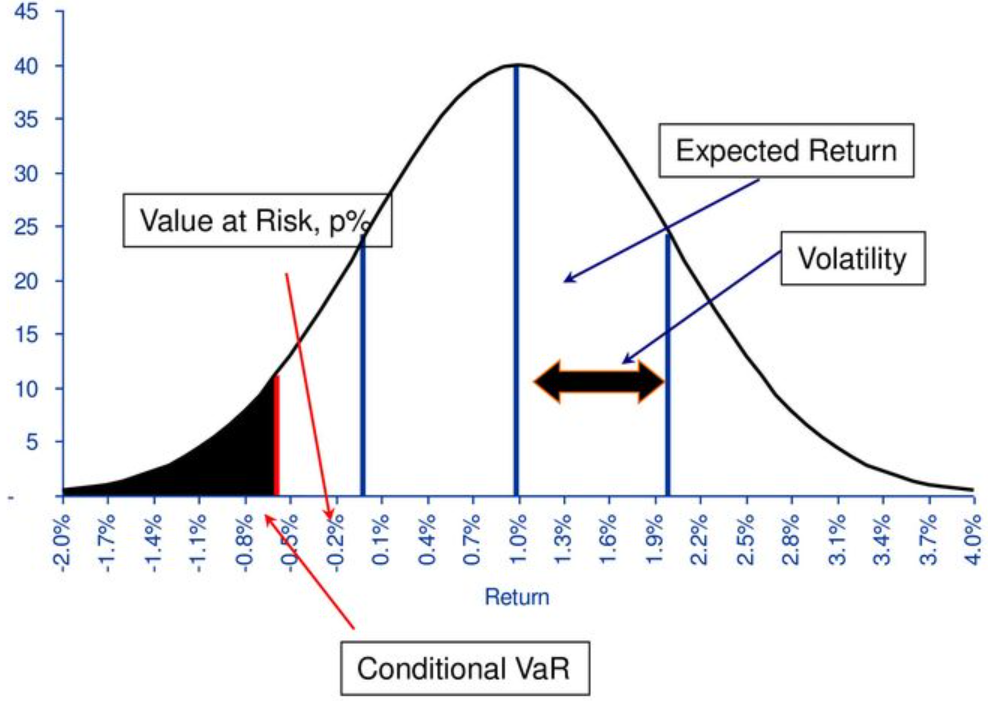
\includegraphics[width= 0.75\textwidth, keepaspectratio]{../output/varconcept.png}
% \caption{Var Concept}
% \source{Source: semanticscholar.com}
% \label{fig:varconcept}
% \end{figure}


A conditional VaR depends on a set  of variables, which can vary in real time.
The distribution on which  the VaR is estimated is based  on the properties of
time  series  and  exogenous   regressors,  thereby  the  term  "conditional."
Following  the literature  \citep{sarno2003},  the dependent  variable is  the
log-return $r_t$ of the exchange rate $e_t$, at a daily frequency (see below).
The   conditional   predictive   density   of   exchange   rate   returns   is
$f(r_{t+1}|X_t)$ where $X_t$ is a vector of explanatory variables.

\begin{equation*}
  r_{t+1} = \log\left(\frac{e_{t+1}}{e_t}\right)
\end{equation*}


The VaR  approach fixes how much  risk remains in  the market and how  much is
absorbed by the central bank. On the contrary, with fixed-volatility triggers,
the risk  transferred to the  central bank varies  with volatility; it  is not
fixed, as with a VaR. The risk removed from the market can be expressed in USD
terms. The  GARCH model  used to  estimate the  model delivers  a full-fledged
conditional  density  of  the  exchange  rate  logreturns.   It  is  therefore
straightforward  to   estimate  the   expected  shortfall  of   exchange  rate
depreciation  or  appreciation  that  the   central  bank  is  preventing  for
occurring. If the central bank knows the aggregate level of FX exposure in the
system, the risk  in USD terms removed  from the market is the  product of the
expected exchange rate shortfall with the system-wide FX exposures.\\


Under the VaR  approach, the policy decision determines how  much risk will be
transferred,  which has  macroeconomic  underpinning.   The quantile  $\theta$
represents the central bank's commitment  to absorb a predetermined portion of
the exchange rate risk. Our model  gives full discretion to the policymaker to
decide on  the risk tolerance.  Conceptually,  the risk tolerance should  be a
function of the pervasiveness of exchange rate exposures in the economy due to
(1) currency mismatches in balance  sheets; and (2) exchange rate pass-through
to  domestic  price.   The  VaR  can  be expressed  as  a  percentage  of  the
distribution or in nominal terms, if  unhedged exposures can be quantified, by
applying  the percentage  to  the  estimated nominal  amount  of the  unhedged
exposure. Then, the VaR  can be presented as a percentage  of GDP to emphasize
macroeconomic implications.\\

Mathematically,  the decision  rule is  formalized as  an intervention  region
$\mathcal{R}_\theta\left(r_t\right)$,   based   on   the   economy   tolerance
thresholds  for  depreciation   and  appreciation,  respectively  ($\theta_l$,
$\theta_u$).    The  decision   rule  is   binary:  if   $r_t$  falls   within
$\mathcal{R}_\theta$,  then the  central bank  intervenes; otherwise,  it does
not. These  regions evolve every day  as a function of  market conditions. For
the rest of the paper, we assume that intervention regions are symmetric, that
is,  unhedged exposures  to  the  exchange appreciation  are  as important  as
unhedged exposures  to depreciation,  to keep  the likelihood  of intervention
against   appreciation   equal   to    the   one   of   intervention   against
depreciation. Other  assumptions can be  made depending  on the nature  of the
risk.

\begin{equation*}
\mathcal{R}_\theta \left(r_t \right) = \left\{r_t \leq Q(r_t | X_{t-1},
    \theta_l) \right\} \cup \left\{r_t > Q(r_t | X_{t-1},
    \theta_u) \right\}
\end{equation*}

Where $Q(r_t |  X_{t-1}, \theta)$ is the $\theta$-quantile  of the conditional
log-returns distribution $f(r_{t+1}|X_t)$.\\

The VaR-based FX interventions formalized above are conceptually appealing, as
they are  rooted in the  principles of  modern financial analysis.  The points
below explain why VaR-based FX intervention complies with these principles:

\begin{itemize}
  
\item  VaR-based FX  interventions  provide an  objectifiable  approach to  FX
interventions by shifting  the policy focus on the exchange  rate risk instead
of the  exchange rate level.  Central banks should  let the market  operate as
long as current FX developments are  within their risk tolerance and intervene
otherwise. Another benefit  of the VaR rule is that  it allows the policymaker
to  anchor its  risk  tolerance  as a  function  of  market and  macroeconomic
conditions (see more discussion below).

\item  VaR-based FX  interventions are  forward-looking, that  is, conditional
VaRs are  forecasted.  Central  bankers should  intervene to  prevent imminent
risks.   Also,   forward-looking  variable  thresholds  reduce   the  risk  of
opportunistic  and strategic  behaviors  from market  participants, who  might
otherwise take speculative positions when the central bank intervenes in fixed
thresholds. Indeed, as market participants are changing behavior, the VaR rule
is changing too.  This complicates  the possibility for market participants to
take speculative  positions, as  they would need  to anticipate  perfectly how
their  new behavior,  as  well as  the  rest  of the  market,  will shift  the
conditional  FX distribution.   On the  contrary, with  fixed thresholds  (for
example, plus or  minus 2 percent), market participants know  exactly when the
central bank will intervene.

\item  VaR-based FX  interventions  are adaptive  to  market conditions.   The
VaR-based triggers loosen or tighten with volatility to keep the likelihood of
FX interventions  unchanged, thereby  accommodating both exchange  rate trends
and changes in volatility regime.  VaR-based FX interventions are, thus, ideal
to accompany the transition to more  exchange rate flexibility in a smooth and
controlled  fashion.   For  example,  policymakers  could  increase  the  risk
tolerance progressively as the FX market depth increases.

\item  VaR-based  FX  interventions  capture the  FX  market’s  nonlinear  and
asymmetric reactions to shocks. Exceeding  a certain level of volatility could
result in sudden shifts in  expectations, closing large positions, and herding
behavior among market participants. Besides,  markets may not react equally to
exchange rate appreciation and depreciation.

\item  VaR-based   FX  interventions  incorporate  information   from  several
indicators. The VaR includes several exogenous variables (for example, bid-ask
spread, FX forward  points, interest rate differential, and so  on) that bring
additional information to the estimation  of the conditional volatility. These
exogenous variables can be  used to factor in the specifics  of a given market
and customize the measure. Our  current modeling approach is parsimonious, but
it  could be  augmented to  incorporate  more complex  models, capturing,  for
example, structural breaks or regime shifts.

\item  VaR-based  FX interventions  support  the  development of  the  hedging
market,  as this  makes sure  that interventions  leave some  risk within  the
market.  The  central  bank  is  not hedging  the  market  against  all  risks
concerning a certain  fixed threshold; it is hedging only  against tail risks,
which are typically  difficult to hedge in  the market. Via the  VaR rule, the
central bank provides a public good  (the hedge), while limiting moral hazards
stemming from  market overconfidence in central  bank interventions. VaR-based
FX interventions also moderate hedging costs  by absorbing some of the risk to
preserve market functioning.

\item Symmetric VaR-based FX interventions are unbiased and budget neutral. If
symmetric, this assumes an equal probability  of buying and selling FX, making
interventions budget  neutral over time.  Besides,  VaR-based FX interventions
avoid  bias  in  the exchange  rate  policy  in  favor  of a  weak  or  strong
currency. However,  asymmetric VaR  rule FX interventions  could be  used, for
example, to  accumulate reserves  by choosing a  higher buying  frequency than
selling.

\item VaR-based  FX interventions derive from  a simple time series  model and
are, therefore, easy to operationalize. The model requires a limited amount of
data,  available   in  the   public  domain,   and  their   interpretation  is
unambiguous. VaR  triggers are transparent  and relatively easy  to understand
and  to  communicate  to  the  market  while  being  part  of  a  more  global
communication  strategy from  the central  bank (see,  for example,  the newly
issued  Central Bank  Transparency Code  published by  the IMF  in 2020).   FX
interventions are  performed on the  wholesale market, where  participants are
aware of the concept of VaR. The  general public might indeed be less familiar
with  the concept,  but  this is  of little  consequence  from an  operational
standpoint. Besides,  technical-based rules  are objective and  strengthen the
independence  of the  central bank  against political  interference, as  these
rules are more difficult to bend.

\item VaR-based  FX interventions are  financially sound for the  central bank
(Annex \ref{sec:fin-perf}).  The central bank  buys and sells  FX with
the  same probability  (if symmetric)  as the  extremes of  the exchange  rate
distribution, and  on the  "good side"  of the  market (selling  expensive and
buying cheap), thereby using its resources efficiently.
\end{itemize}


%% ---------------------------------------------------------------------------
%% Empirical Framework
%% ---------------------------------------------------------------------------
\section{Empirical Framework}
\label{sec:empirical-framework}

\subsection{Specification}
\label{sec:specification}

A nonlinear univariate EGARCH-X model  is used to estimate the forward-looking
exchange  rate  Value at  Risk  $Q\left(r_t\  \right|\ t-1,\  \theta)$.   More
precisely,  the  VaR-based  FX  interventions model  presented  here  uses  an
Exponential  GARCH  (EGARCH) model  of  volatility  with exogenous  regressors
(EGARCH-X) to adequately capture nonlinearities and asymmetries. The advantage
of the  EGARCH-X model is  that it is a  relatively parsimonious model,  as it
incorporates  nonlinearities and  asymmetries with  only two  equations. GARCH
models are also very stable, and easy to implement and to understand, compared
with more complex  forecasting models. Besides, the literature  has shown that
GARCH  models have  very decent  forecasting performances  in the  case of  FX
markets (see, for example, \cite{mcmillan2012}).\\

That  being  said,   other  models  (such  as   copulas,  kernel  regressions,
time-varying coefficient  models, and  so on)  could be  used to  estimate the
conditional distribution in real time, and even intraday.  The model presented
here is a proof of concept and could be refined by the central bank for actual
implementation and  operational work.   The EGARCH  specification incorporates
three components: drift,  volatility, and the distribution of  the error terms
or innovations.\\


\begin{itemize}
\item \textbf{Drift}: $r_t= \bm{Intercept} + \bm{\rho} r_{t-1} + \bm{\beta}
X_t + \varepsilon_t$ AR-X(p) for the average level of log-returns ($r_t$, the
drift), and  $X_t$ a vector of  exogenous regressors.  The drift  reflects the
conditional exchange rate trend

\item \textbf{Volatility}: $\log \sigma_t^2 = \bm{\omega} + \bm{\beta} g(r_{t-1}) \text{with} \
  g(r_t)= \bm{\alpha} r_t + \bm{\gamma}(|r_t| - \mathbb{E}[|r_t|])$: where $\sigma_t$  is
  the volatility 

\item \textbf{Errors term}: $\varepsilon_t = \sigma_t \epsilon_t,\ \epsilon_t \sim TSK\
(\bm{\nu}, \bm{\lambda})$: the error term is parameterized for instance with
a Tskew  distribution (other  distributions can be  used, including  Normal, T
distribution and generalized error distributions).
  
\end{itemize}

The parameters in \textbf{bold} are estimated by the GARCH model.\\

The  estimates  use  an  EGARCH-X(1,1)  with  Tskew  distributed  innovations,
estimated  via  Maximum  Likelihood  Estimation.\footnote{We  built  a  Python
wrapper around  the comprehensive  "ARCH" Python  package, developed  by Kevin
Sheppard  from Oxford  University  \citep{sheppard2020}} The  public data  and
Python  codes  to  replicate  the  results of  this  paper  are  available  at
\url{https://romainlafarguette.github.io/software/}   GARCH   models   are   a
standard approach to estimating  and forecasting volatility \citep{engle2001}.
The number  and order  of lags  are chosen based  on AIC/BIC  criteria (Akaike
Information Criterion/Bayesian Information  Criterion).  An alternative model
is  the  JP  Morgan  RiskMetrics model  \citep{zumbach2007},  with  exogeneous
regressors and  innovations distributed  with generalized  error distribution,
also   known   as   generalized   Gaussian   distribution   (GGD).    Annex
\ref{sec:benchmarking}  presents  different   specifications  and  alternative
models as a robustness exercise.\\

Exogeneous  regressors  are incorporated  into  the  model to  capture  market
microstructures,  interest  rate  parity,  and  international  risk  sentiment
factors. The  objective is to  add more information  in the estimation  of the
VaR,  thereby  refining  the  estimation of  FX  intervention  triggers.  This
approach  is  advantageous because  it  combines  the information  of  several
intervention indicators in  a single measure. Although our  estimation is done
at the daily  level, we incorporated some proxies for  intraday volatility and
liquidity. The estimates include the following regressors:

\begin{itemize}
\item \textbf{The average exchange rate bid-ask spread over the day}, taken in
  absolute terms. The finance literature uses the bid-ask spread as a proxy of
  intraday market liquidity
\item \textbf{The intraday spread (max–min over the day)}, which is another
  metric of intraday volatility
\item \textbf{The daily  interest rate differential between  local and foreign
currencies} captures  the interest  rate parity arbitrage.  We used  the daily
interest rate  differential instead of  the cross-currency basis swap,  as the
former has a longer available time series
\item \textbf{The  one-month forward  exchange rate},  expressed as  the first
difference from the day before. As the previous variable controls for interest
rate parity, the forward rate could capture  the impact of the cost of hedging
on the spot market
\item \textbf{The first-difference variation of the VIX}, which captures
  global risk sentiment.\footnote{We tried with the CBOE Volatility Index
    (VIX) in level, but the p-value was higher than in the first difference}
\item \textbf{The exchange rate of the US dollar vis-à-vis the euro}, to
  control for US dollar specific developments
\item \textbf{Oil prices log returns}, as Mexico is an oil exporter and oil
  prices could impact the exchange rate
\end{itemize}


\subsection{Estimation Results}
\label{sec:estimation-results}

As a proof of concept, the model is  fitted against a real sample of Mexico FX
data (against  the US  dollar) since  2001. The peso  has been  floating since
1994.   Figure  \ref{fig:descriptive-plot}   presents  the  historical  level,
returns,  and  returns distribution  of  exchange  rate.  The  bilateral  spot
exchange rate  exhibits significant  volatility in crisis  times, such  as the
global financial crisis of 2008 and, more recently, the COVID-19 pandemic. The
historical  distribution  shows that  the  returns  are  skewed to  the  right
(depreciation). The model thus  incorporates asymmetries to accurately capture
the dynamics of this exchange rate  series. Intervention data are available on
the                                                                       BM's
website.\footnote{\url{https://www.banxico.org.mx/mercados/subastas-cambio-credito-banco.html.}}\\

\begin{figure}
  \centering
  \caption{Mexican Peso against US Dollar}
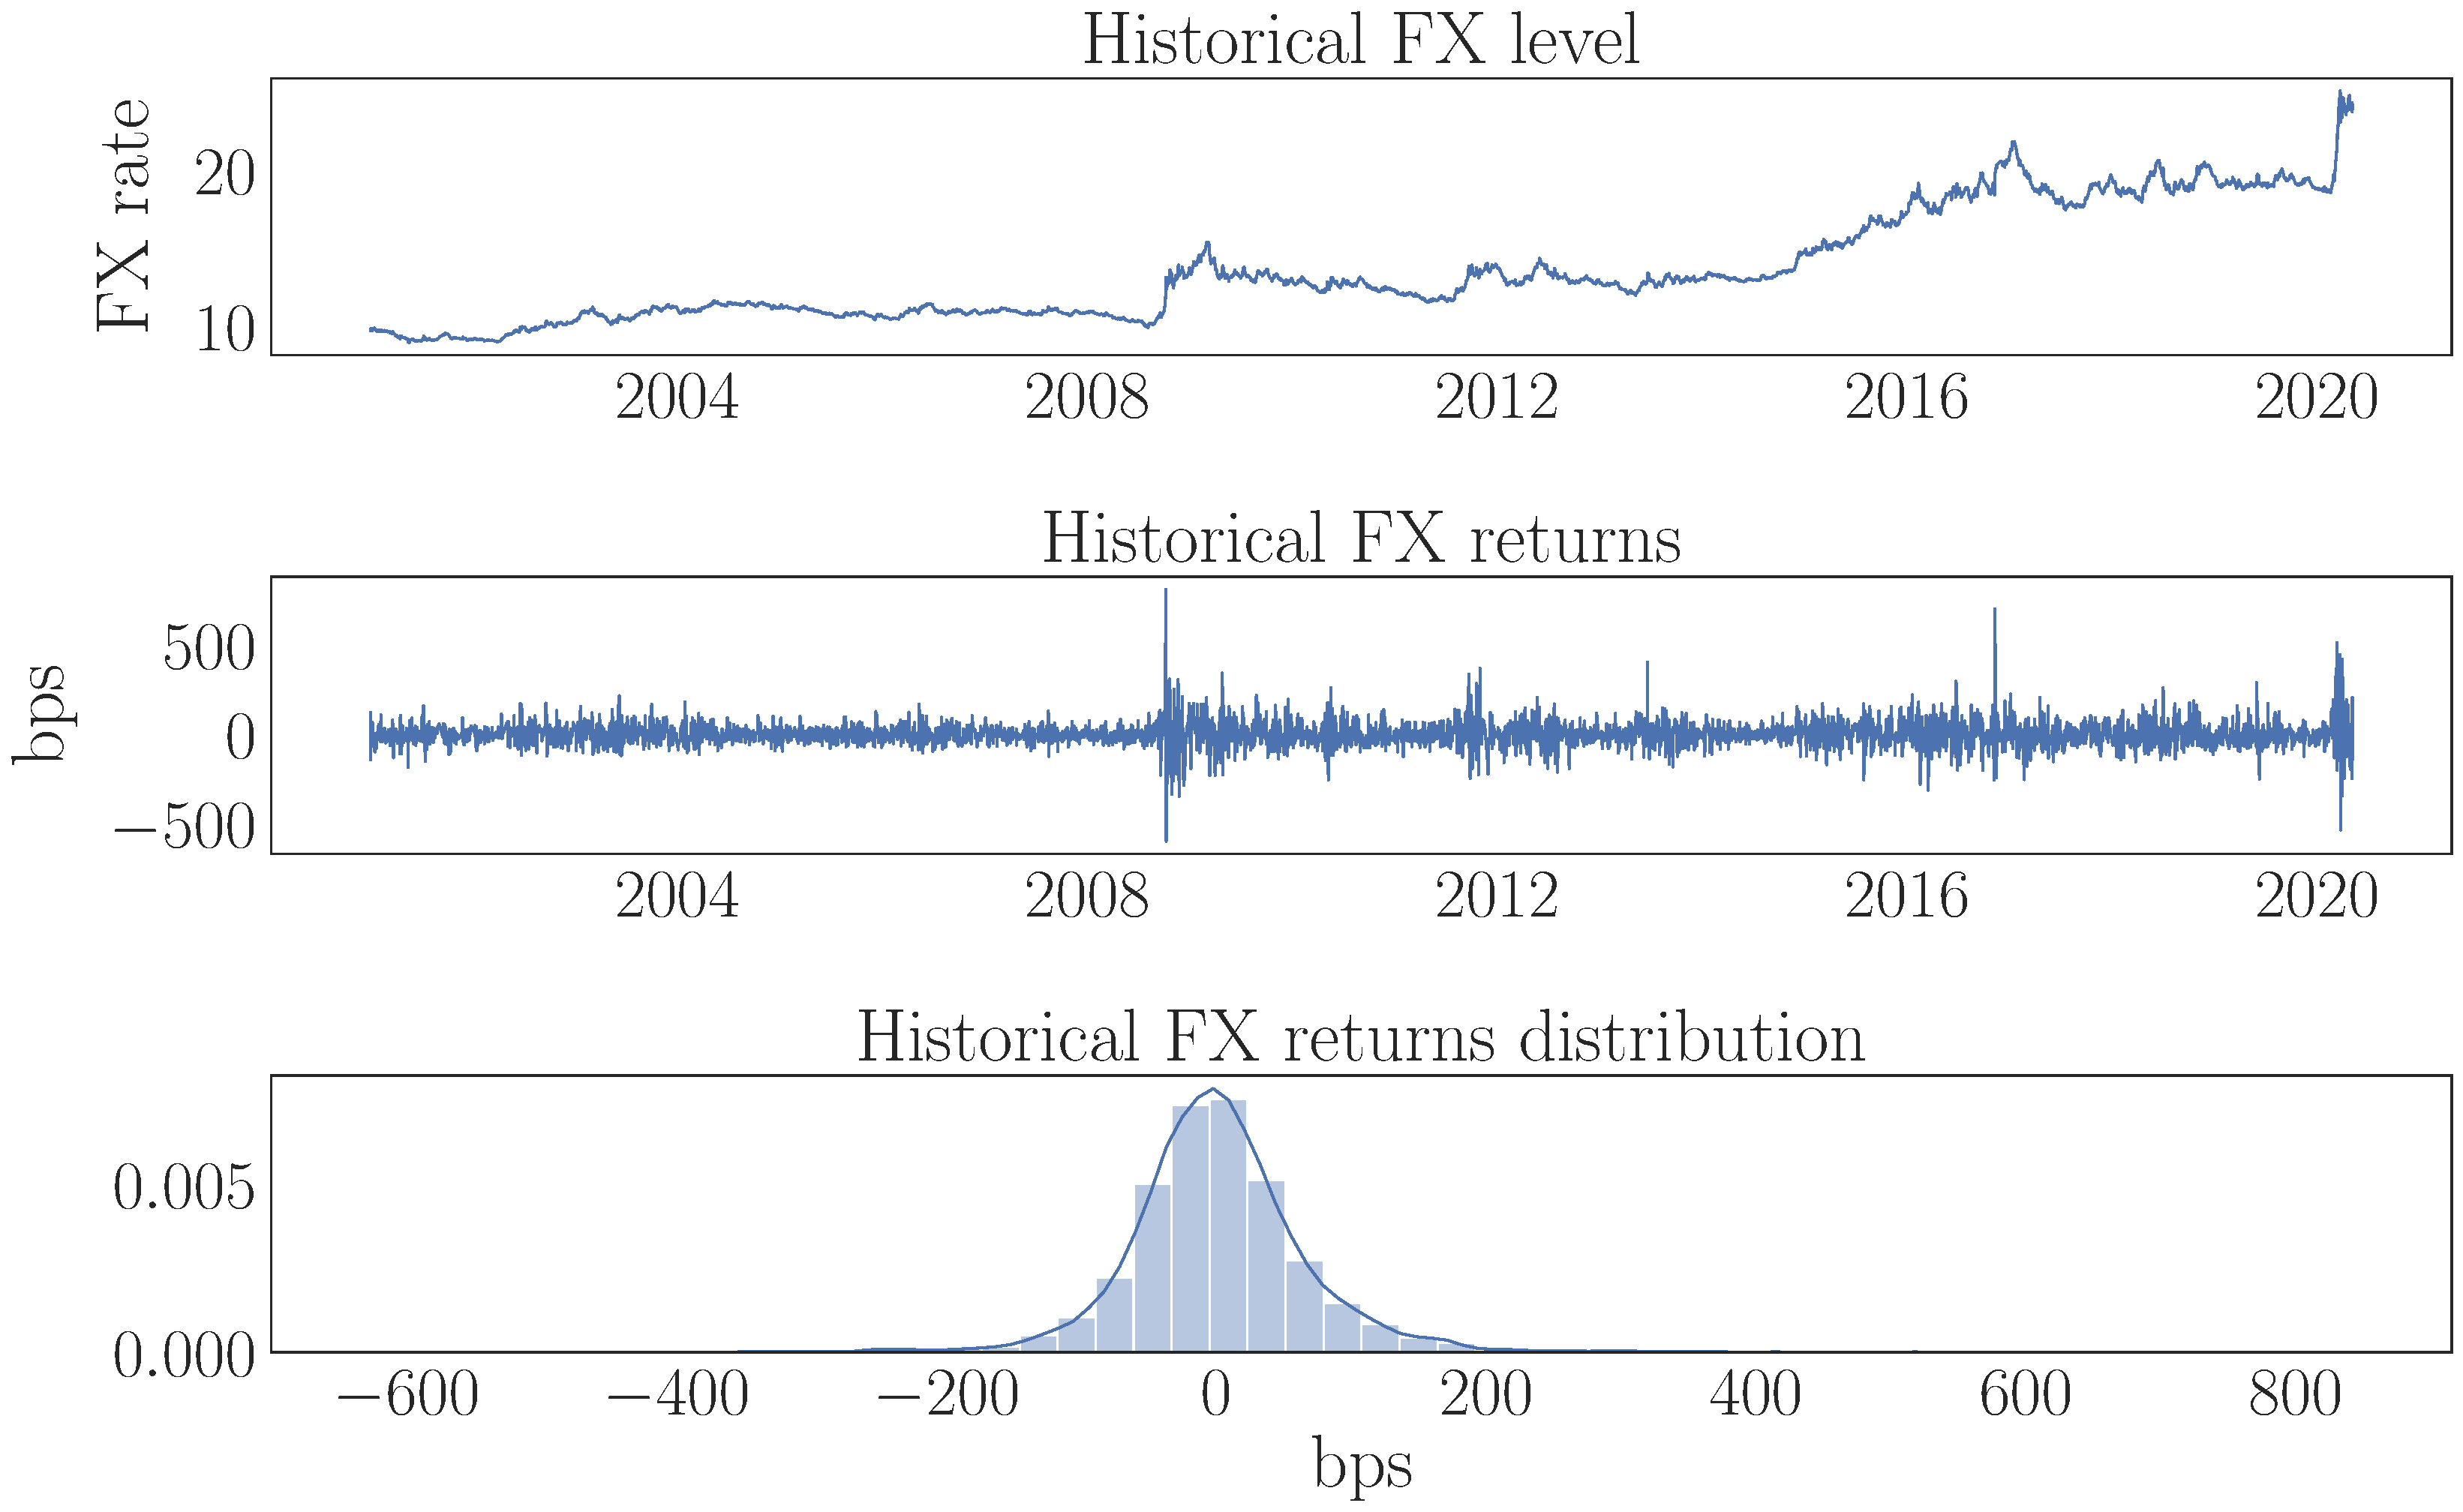
\includegraphics[width= 0.95\textwidth, keepaspectratio]{../output/descriptive_plot.pdf}
\label{fig:descriptive-plot}
\source{\emph{Sources}: Bloomberg and authors' calculations}
\end{figure}


The signs  of the coefficients  are consistent with macroeconomic  and finance
theory   (see   \cite{sarno2003}   for   an  exposition   of   exchange   rate
economics).  Table  \ref{tab:reg-coeffs}  presents  the output  of  the  GARCH
estimation process,  where we  integrate progressively the  coefficients under
different specifications,  starting from  the micro to  the macro  factors. We
have tried to  insert year dummies to control for  structural breaks, but most
of the coefficients were insignificant.\\

\begin{itemize}
\item The bid-ask spread is positively correlated, suggesting that an increase
  in the bid-ask spread (market illiquidity) signals depreciation
  
\item Forward points also contribute to predicting the movement in exchange
  rate log returns, with the same sign as expected
  
\item A positive interest rate differential with the London Interbank Offered
  Rate (LIBOR) tends to appreciate the currency, due to carry-trade arbitrage
  
\item The same results hold for the CBOE Volatility Index (VIX), as an
  increase in global risk sentiment tends to depreciate emerging market
  currencies
  
\item Changes in the EUR/USD exchange rate have the expected impact on local
  currency returns and contribute to the explanatory power of the
  model. Similarly, with the oil price log returns, an increase in oil prices
  is associated with an appreciation of the local currency against the USD
  
\item The model explains around 28 percent of the log-return variance
\end{itemize}

\begin{table}
  \begin{center}
    \caption{Results of the GARCH Estimates}
%\footnotesize  %%  command to change the font size
\begin{tabular}{llllll}
\toprule
{} & Microstructure &       CIP & Dollar move & Risk Appetite &  Baseline \\
\midrule
Intercept                       &       -2.33*** &     -2.29 &       -1.84 &         -2.55 &     -1.63 \\
Lag FX log returns              &       -0.07*** &     -0.08 &    -0.08*** &      -0.08*** &  -0.08*** \\
Bid ask abs                     &           5.71 &     24.39 &      -35.66 &         -2.42 &      3.23 \\
Min max abs                     &       35.56*** &     34.63 &       34.32 &        34.55* &     26.21 \\
Forward points first difference &       23.29*** &  17.79*** &    26.44*** &       19.8*** &  19.44*** \\
Interbank rate vs Libor         &                &  33.61*** &    39.32*** &      34.75*** &  33.86*** \\
EURUSD log returns              &                &           &    -0.14*** &      -0.17*** &  -0.16*** \\
VIX first diff                  &                &           &             &      15.66*** &  15.37*** \\
FX intervention dummy lag       &                &           &             &               &      2.23 \\
Oil prices log returns          &                &           &             &               &  -0.02*** \\
Omega                           &        0.13*** &      0.13 &     0.12*** &       0.11*** &   0.12*** \\
Alpha                           &        0.17*** &     0.17* &     0.16*** &       0.16*** &   0.15*** \\
Gamma                           &        0.07*** &   0.06*** &     0.06*** &       0.05*** &   0.05*** \\
Beta                            &        0.98*** &   0.99*** &     0.99*** &       0.99*** &   0.99*** \\
Nu                              &        8.33*** &   8.66*** &     8.92*** &       8.71*** &   8.54*** \\
Lambda                          &        0.08*** &      0.07 &        0.09 &         0.07* &   0.08*** \\
R2                              &          5.8 \% &     6.7 \% &      10.4 \% &        27.3 \% &    27.6 \% \\
R2 adjusted                     &          5.8 \% &     6.6 \% &      10.4 \% &        27.2 \% &    27.5 \% \\
Number of observations          &           5986 &      5986 &        5682 &          5682 &      5680 \\
Significance *10\%, **5\%, ***1\%  &                &           &             &               &           \\
\bottomrule
\end{tabular}

%\normalsize
\source{\emph{Sources}: authors’ calculations}
\label{tab:reg-coeffs}
\end{center}
\end{table}


Once  fitted,  the  GARCH  model  provides  an  in-sample  estimation  of  the
conditional  volatility,   $\sigma_t^2$,  over   time,  presented   in  Figure
\ref{fig:conditional-vol}.   Not   surprisingly,  the   in-sample  conditional
volatility  spikes  during  the  global  financial  crisis  and  the  COVID-19
crisis.\\

\begin{figure}
  \centering
  \caption{Conditional FX Volatility over Time}
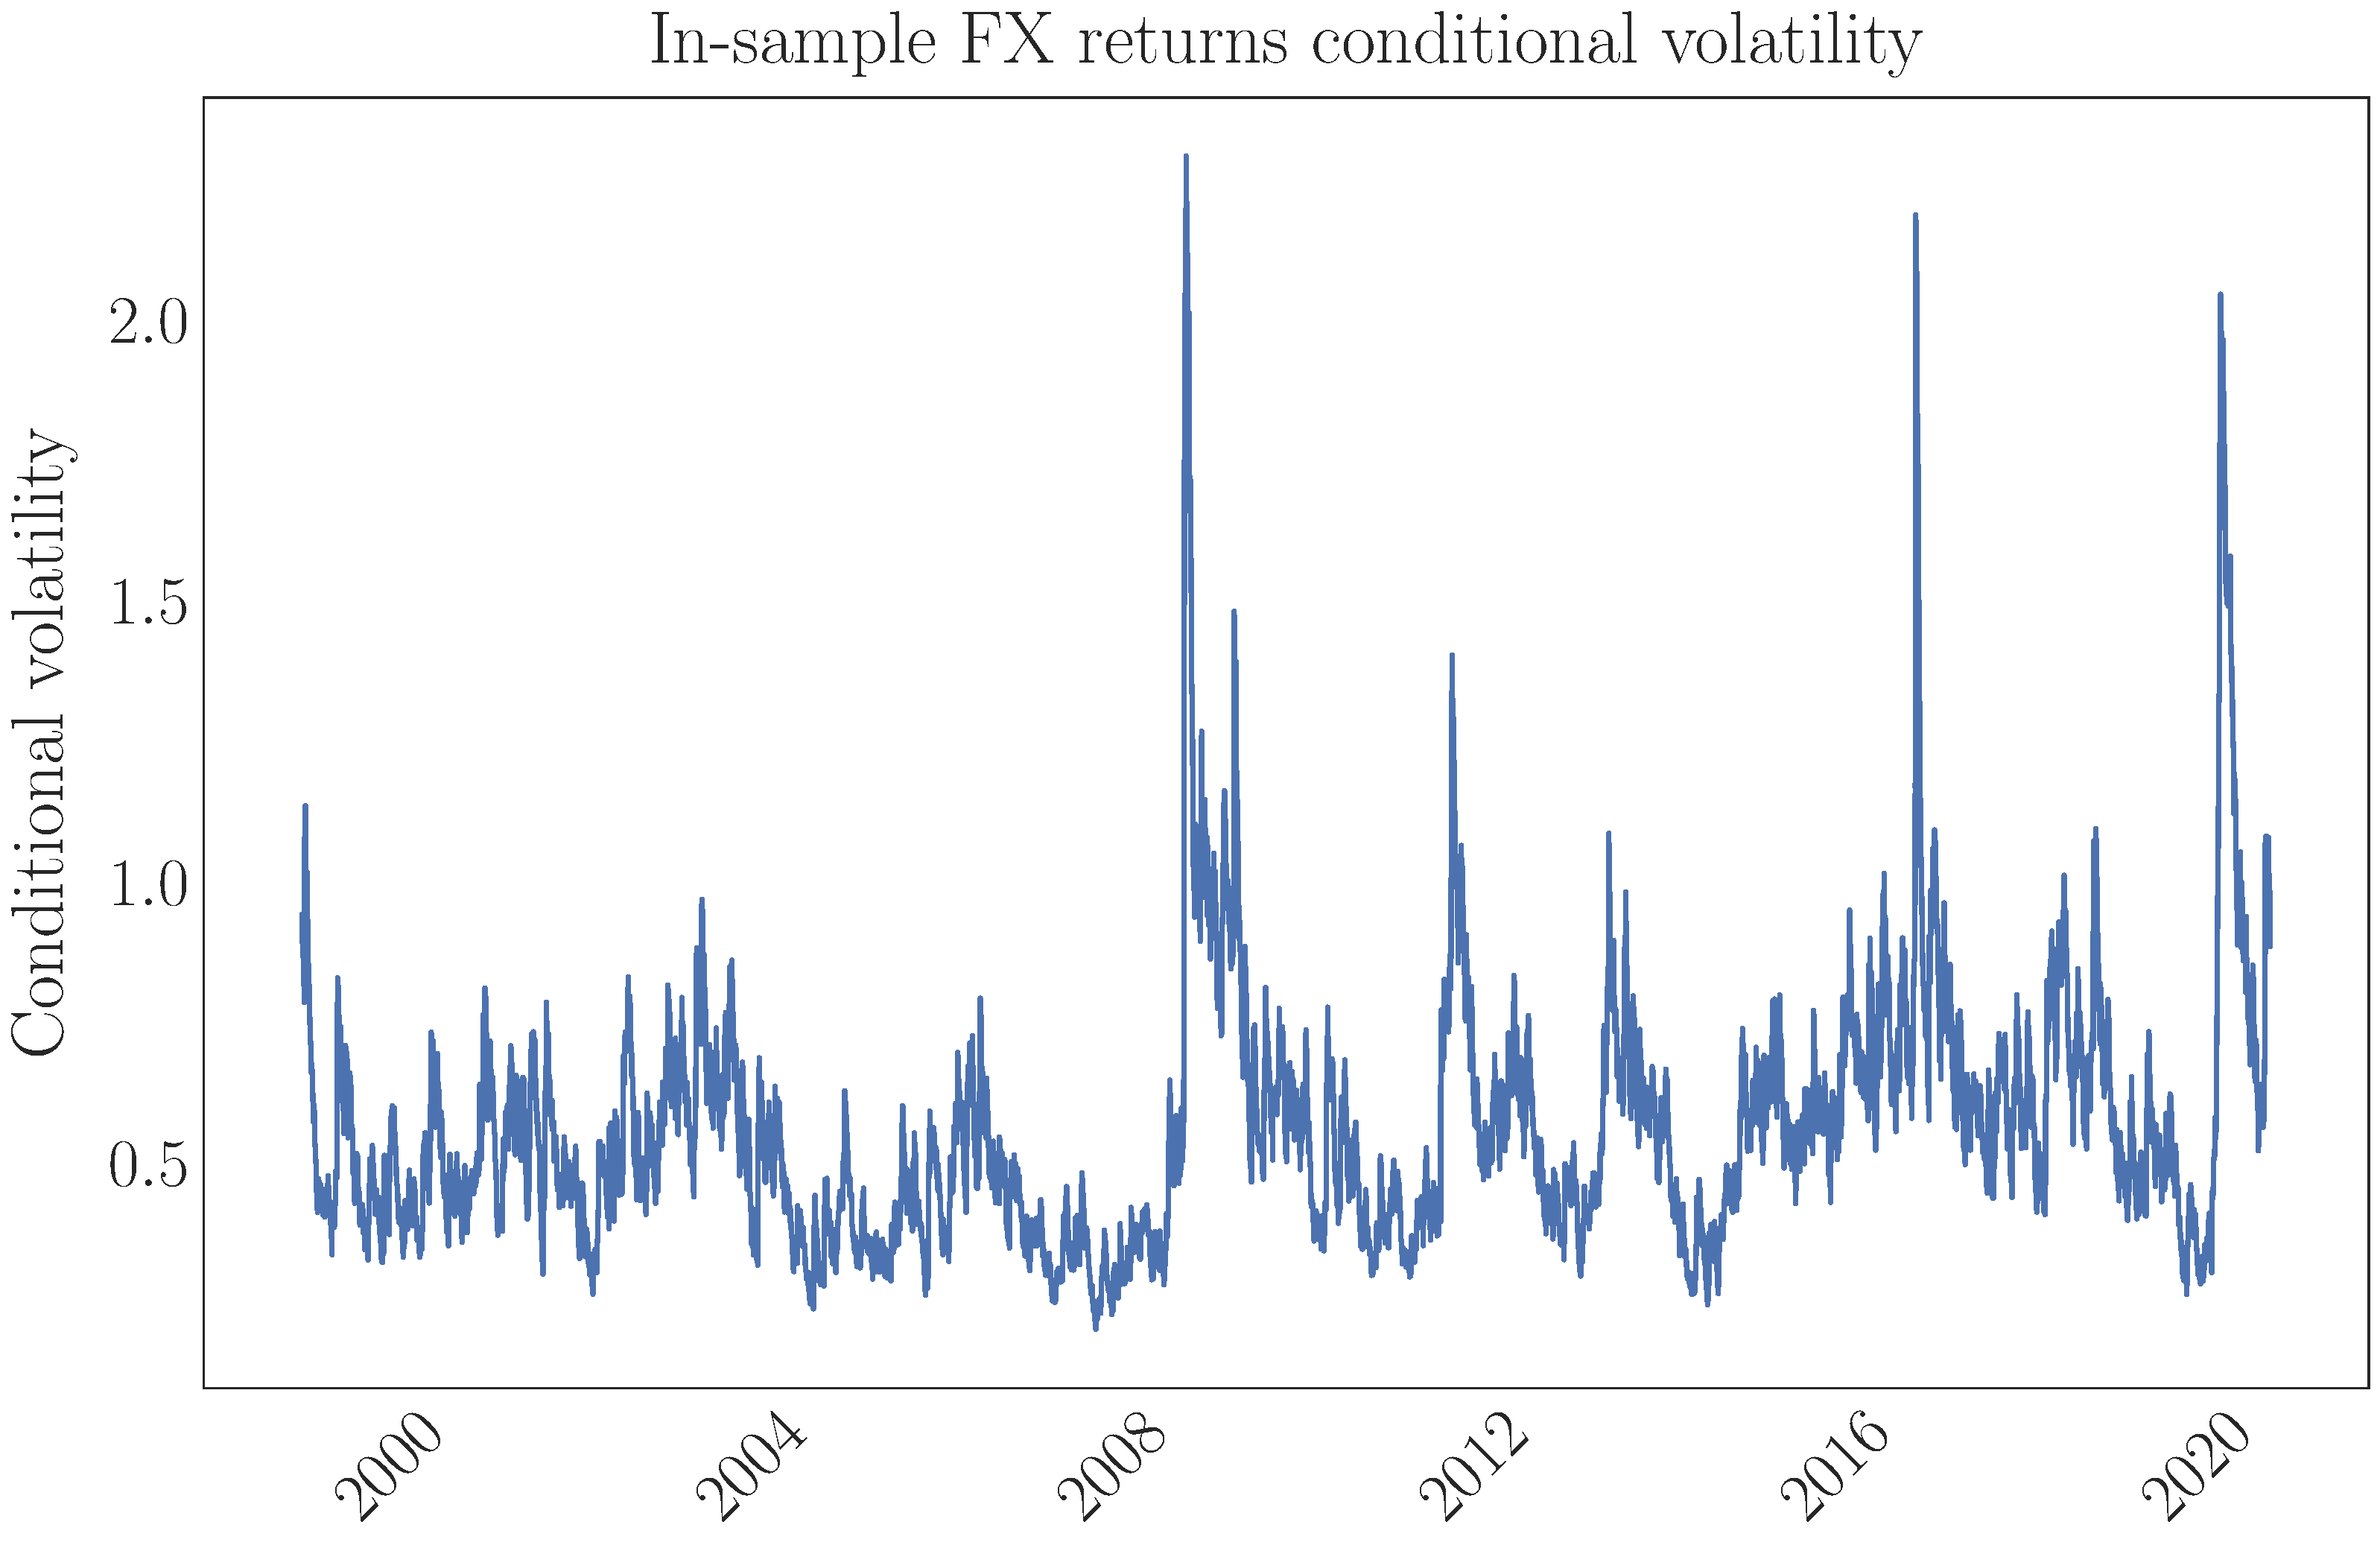
\includegraphics[width= 0.95\textwidth, keepaspectratio]{../output/conditional_vol_plot.pdf}
\label{fig:conditional-vol}
\source{\emph{Sources}: authors' calculations}
\end{figure}


Figure  \ref{fig:joyplot} presents  an out-of-sample  plot of  the conditional
density,  estimated through  the fitted  GARCH via  expanding windows,  over a
10-month timeframe  (from January through  end-October 2020). The plot  of the
conditional  density shows  that not  only the  conditional volatility  widens
significantly  during  the COVID-19  crisis  (in  March  2020), but  that  the
skewness varies also substantially.\\

\begin{figure}
  \centering
  \caption{Out-of-Sample Conditional Density}
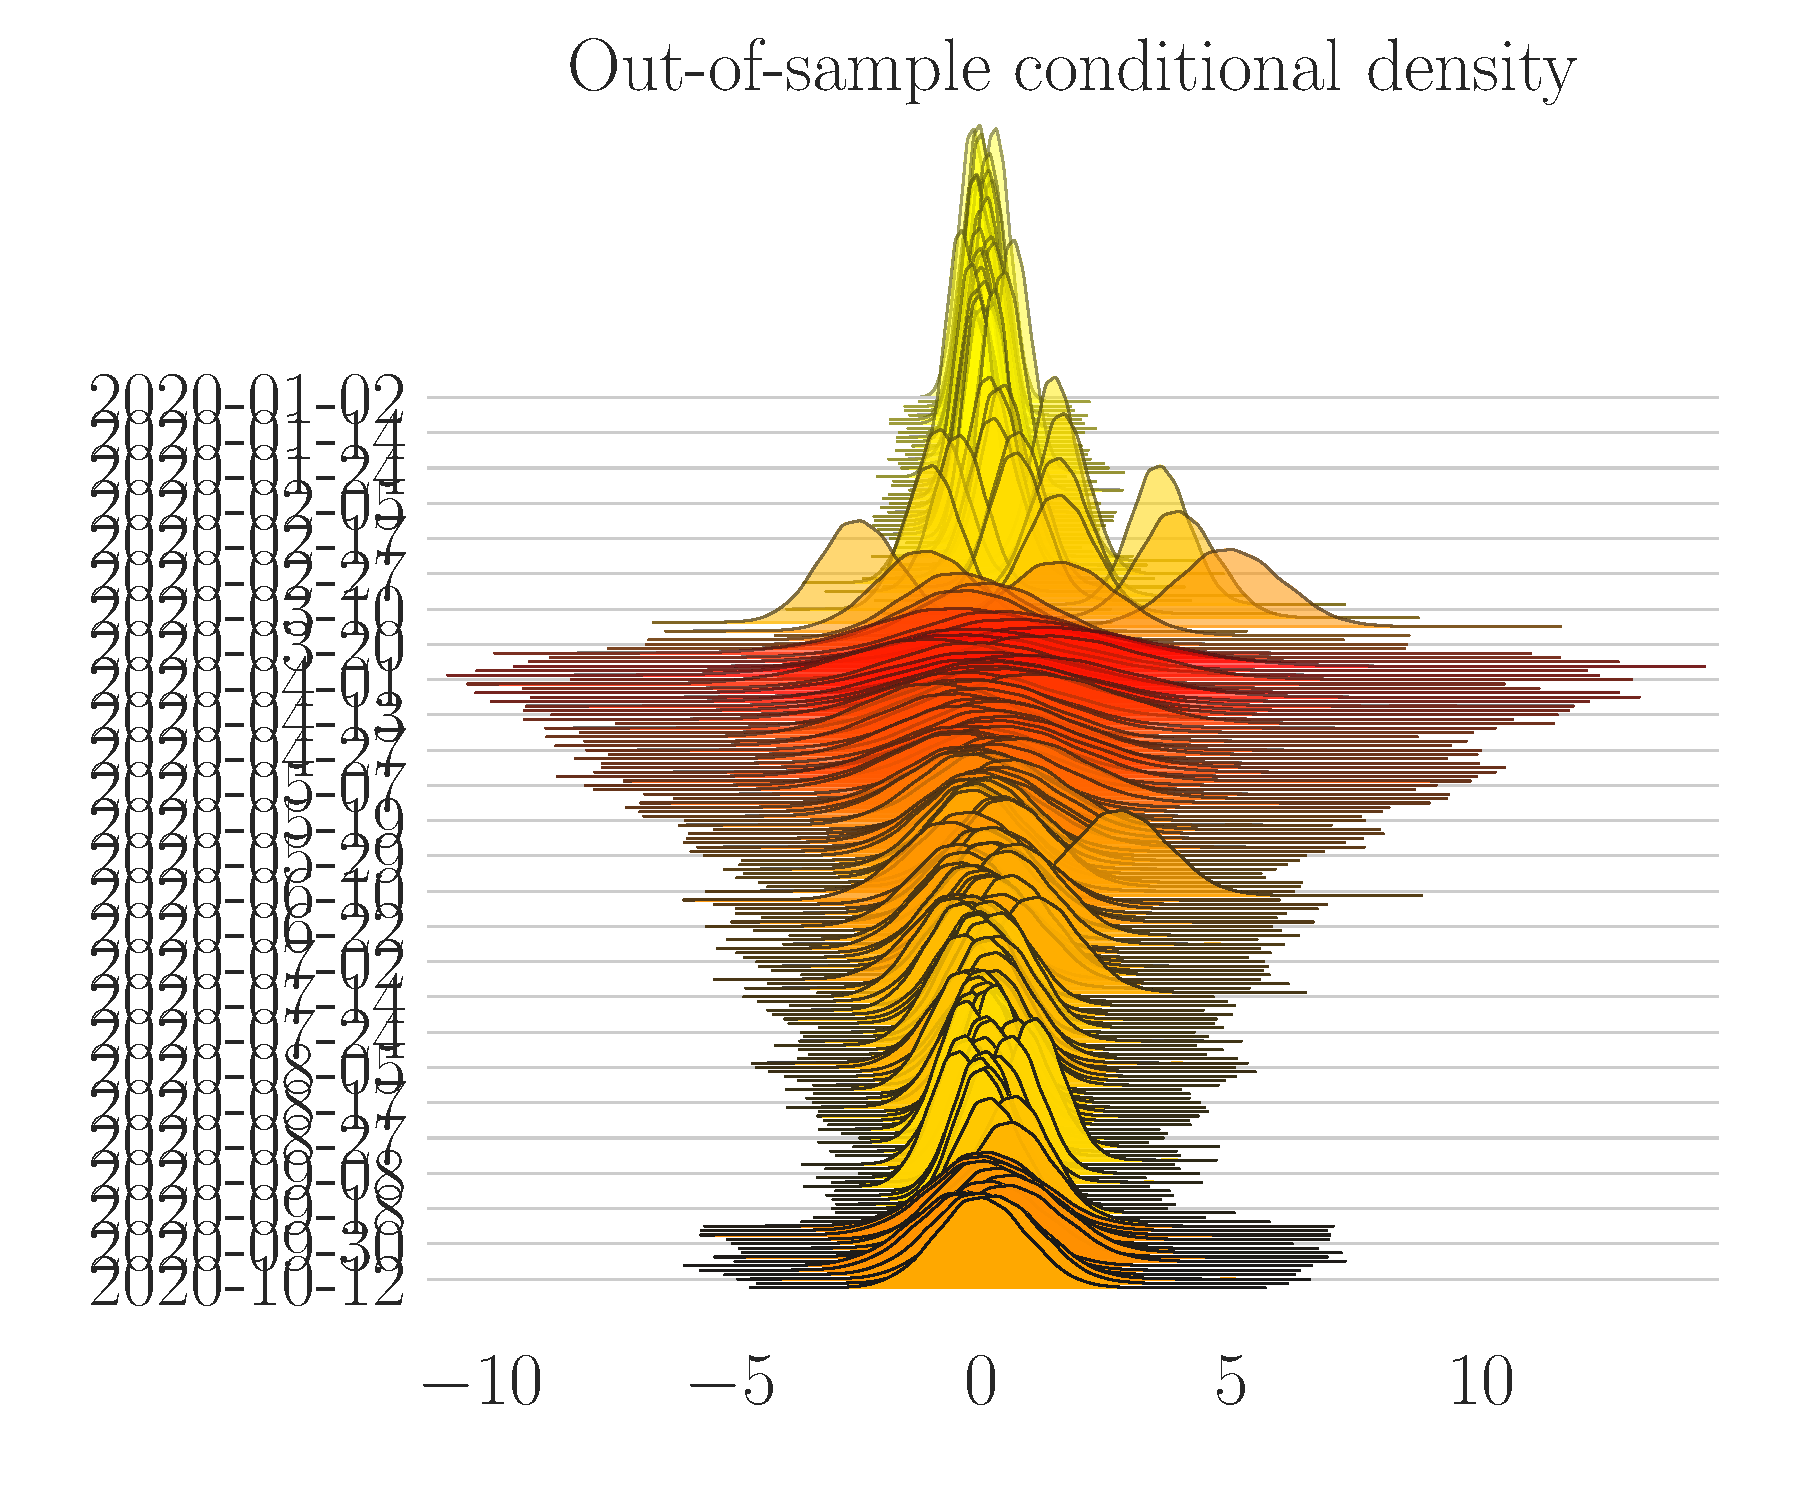
\includegraphics[width= 0.95\textwidth, keepaspectratio]{../output/joyplot.pdf}
\label{fig:joyplot}
\source{\emph{Sources}: authors' calculations}
\end{figure}


Like other  types of forecasting density  models, the GARCH model  can also be
used   to   produce  the   so-called   fan   charts,   as  shown   in   Figure
\ref{fig:fanchart}. The  fan chart  presents the  forecasted quantiles  of the
conditional  distribution  across  time  and  provides  an  intuitive  way  to
understand the uncertainty surrounding the  mean forecasts.  In this case, the
uncertainty  is  precisely captured  by  the  GARCH  model, both  through  the
estimation  of the  conditional density  and also  via higher  moments of  the
distribution, including the skewness.\\

\begin{figure}
  \centering
  \caption{Out-of-Sample Fan Chart}
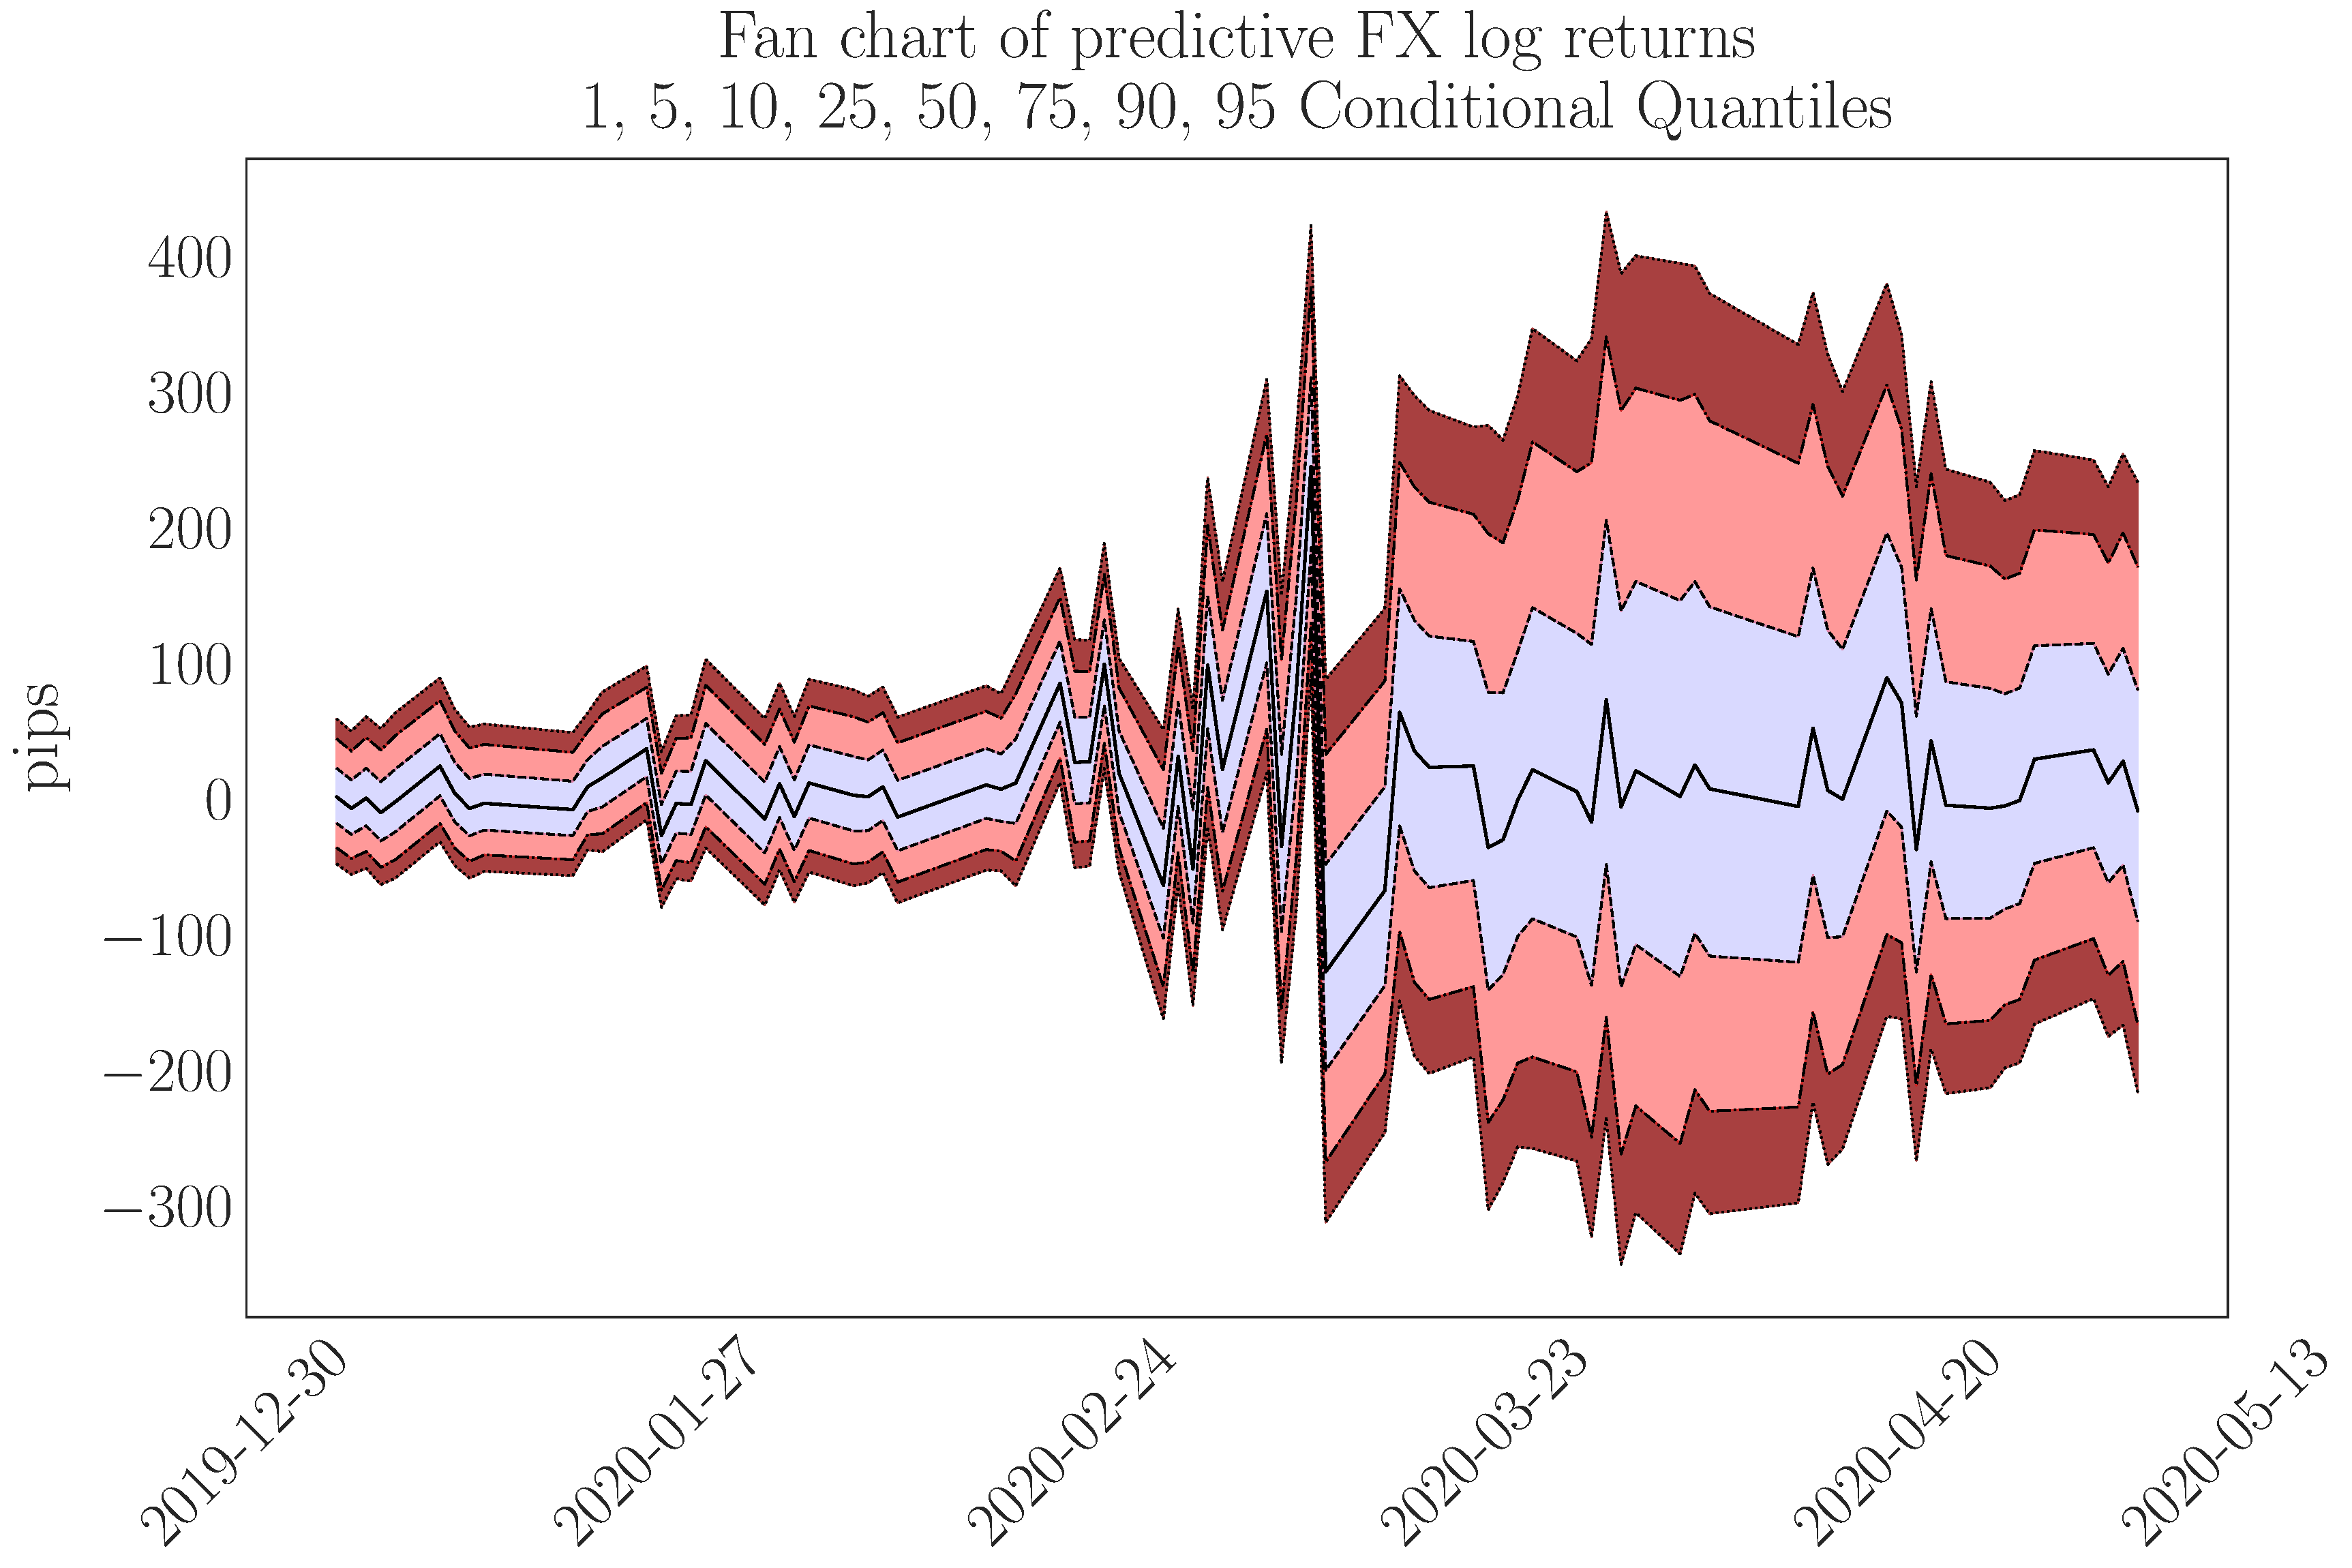
\includegraphics[width= 0.95\textwidth, keepaspectratio]{../output/fanchart.pdf}
\label{fig:fanchart}
\source{\emph{Sources}: authors' calculations}
\end{figure}

Finally,  the quality  of the  GARCH  forecasting density  model is  evaluated
out-of-sample. The correctness of the  density model specification is assessed
via  a   probability  integral   transform  (PIT)   test  (\cite{diebold1998};
\cite{rossi2019}).  The  PIT test  is evaluated over  four-month out-of-sample
daily data,  as presented in  Figure \ref{fig:pitchart}. The PIT  test outcome
presented   in  Figure   \ref{fig:pitchart}  indicates   that  the   empirical
distribution of the PIT is within the confidence band for all quantiles.  This
pattern suggests that the conditional density derived from the EGARCH-X models
has  a  satisfactory  out-of-sample  accuracy and  that  it  generates  robust
predictive distributions  that capture well  upside and downside  risks. Annex
\ref{sec:benchmarking} presents a series of alternative models (unconditional,
quantile  regressions, variation  around GARCH,  and so  on) to  benchmark the
performance of  our model,  also using log  score performance  metrics against
other models.   The result  of the tests  is that the  GARCH family  of models
dominates  the  alternative tested  against  an  unconditional kernel  density
estimator  and conditional  density  estimated from  the quantile  regression.
Also, within  the GARCH family (Gaussian,  Tskew, GARCH versus EGARCH,  and so
on), there is  no significant improvement in performance  against our baseline
model.\\


\begin{figure}
  \centering
  \caption{Probability Integral Transform Test}
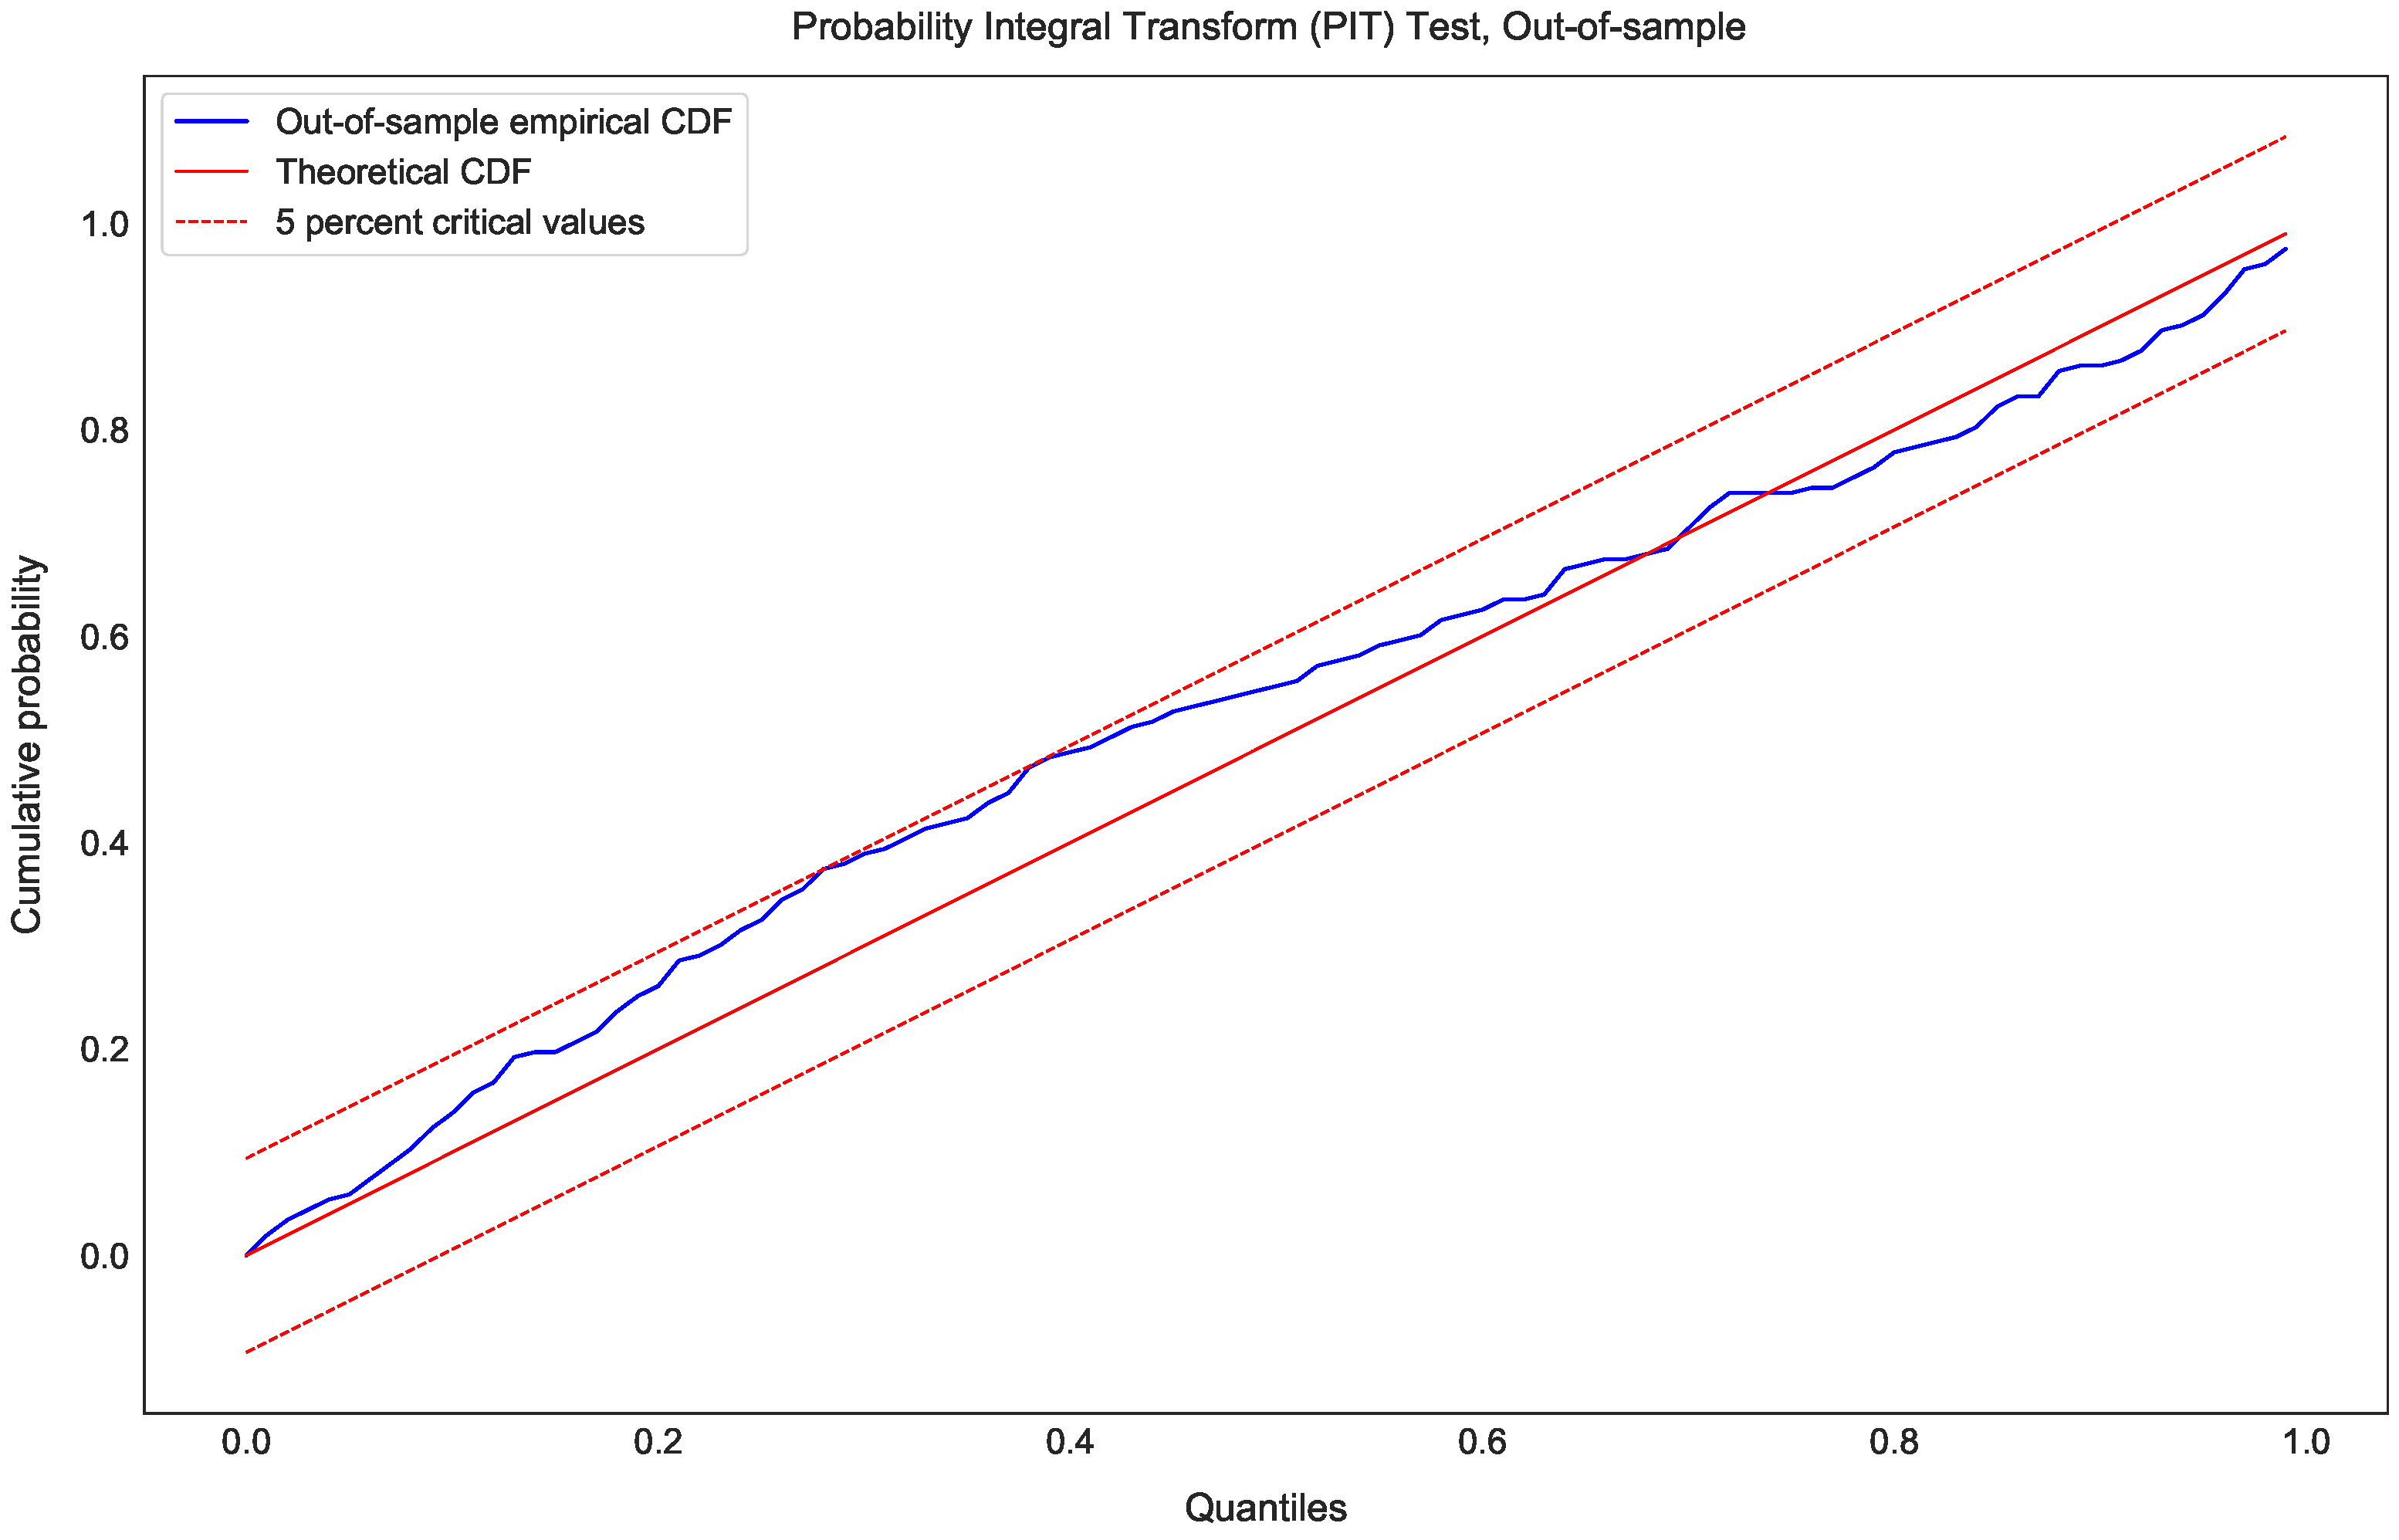
\includegraphics[width= 0.95\textwidth, keepaspectratio]{../output/pitchart.pdf}
\label{fig:pitchart}
\source{\emph{Sources}: authors' calculations}
\end{figure}



%% ---------------------------------------------------------------------------
%% Operational Framework
%% ---------------------------------------------------------------------------
\section{Operational Framework}
\label{sec:operational-framework}


\subsection{Risk-Based Triggers}
\label{sec:triggers}

From  the forecasted  conditional VaR,  it is  straightforward to  infer daily
intervention  regions  for  depreciation  and appreciation,  as  explained  in
Section \ref{sec:var-interventions}.  In  practical terms, at the  end of each
day, the  central bank  re-estimates the model  and assesses  the intervention
regions  for the  day  after.  On  that  day, the  central  bank monitors  the
cumulated   returns    of   the    exchange   rate—either    depreciation   or
appreciation. Once the  cumulated returns reach the  intervention regions, the
central bank buys or  sells FX.  These regions evolve every  day as a function
of   market   conditions.   On   the  specific   day   presented   in   Figure
\ref{fig:var-rule}, intervention happens only if the exchange rate depreciates
by more  than 3.3 percent  or appreciates  by more than  3.7 percent, for  a 5
percent ERaR  (2.5 percent on each  side).  However, a new  threshold would be
computed every  day, for  each possible  quantile, as shown  on the  fan chart
(Figure \ref{fig:fanchart}).\\

\begin{figure}
  \centering
  \caption{VaR FX Intervention Rule Based on a Given Information Set}
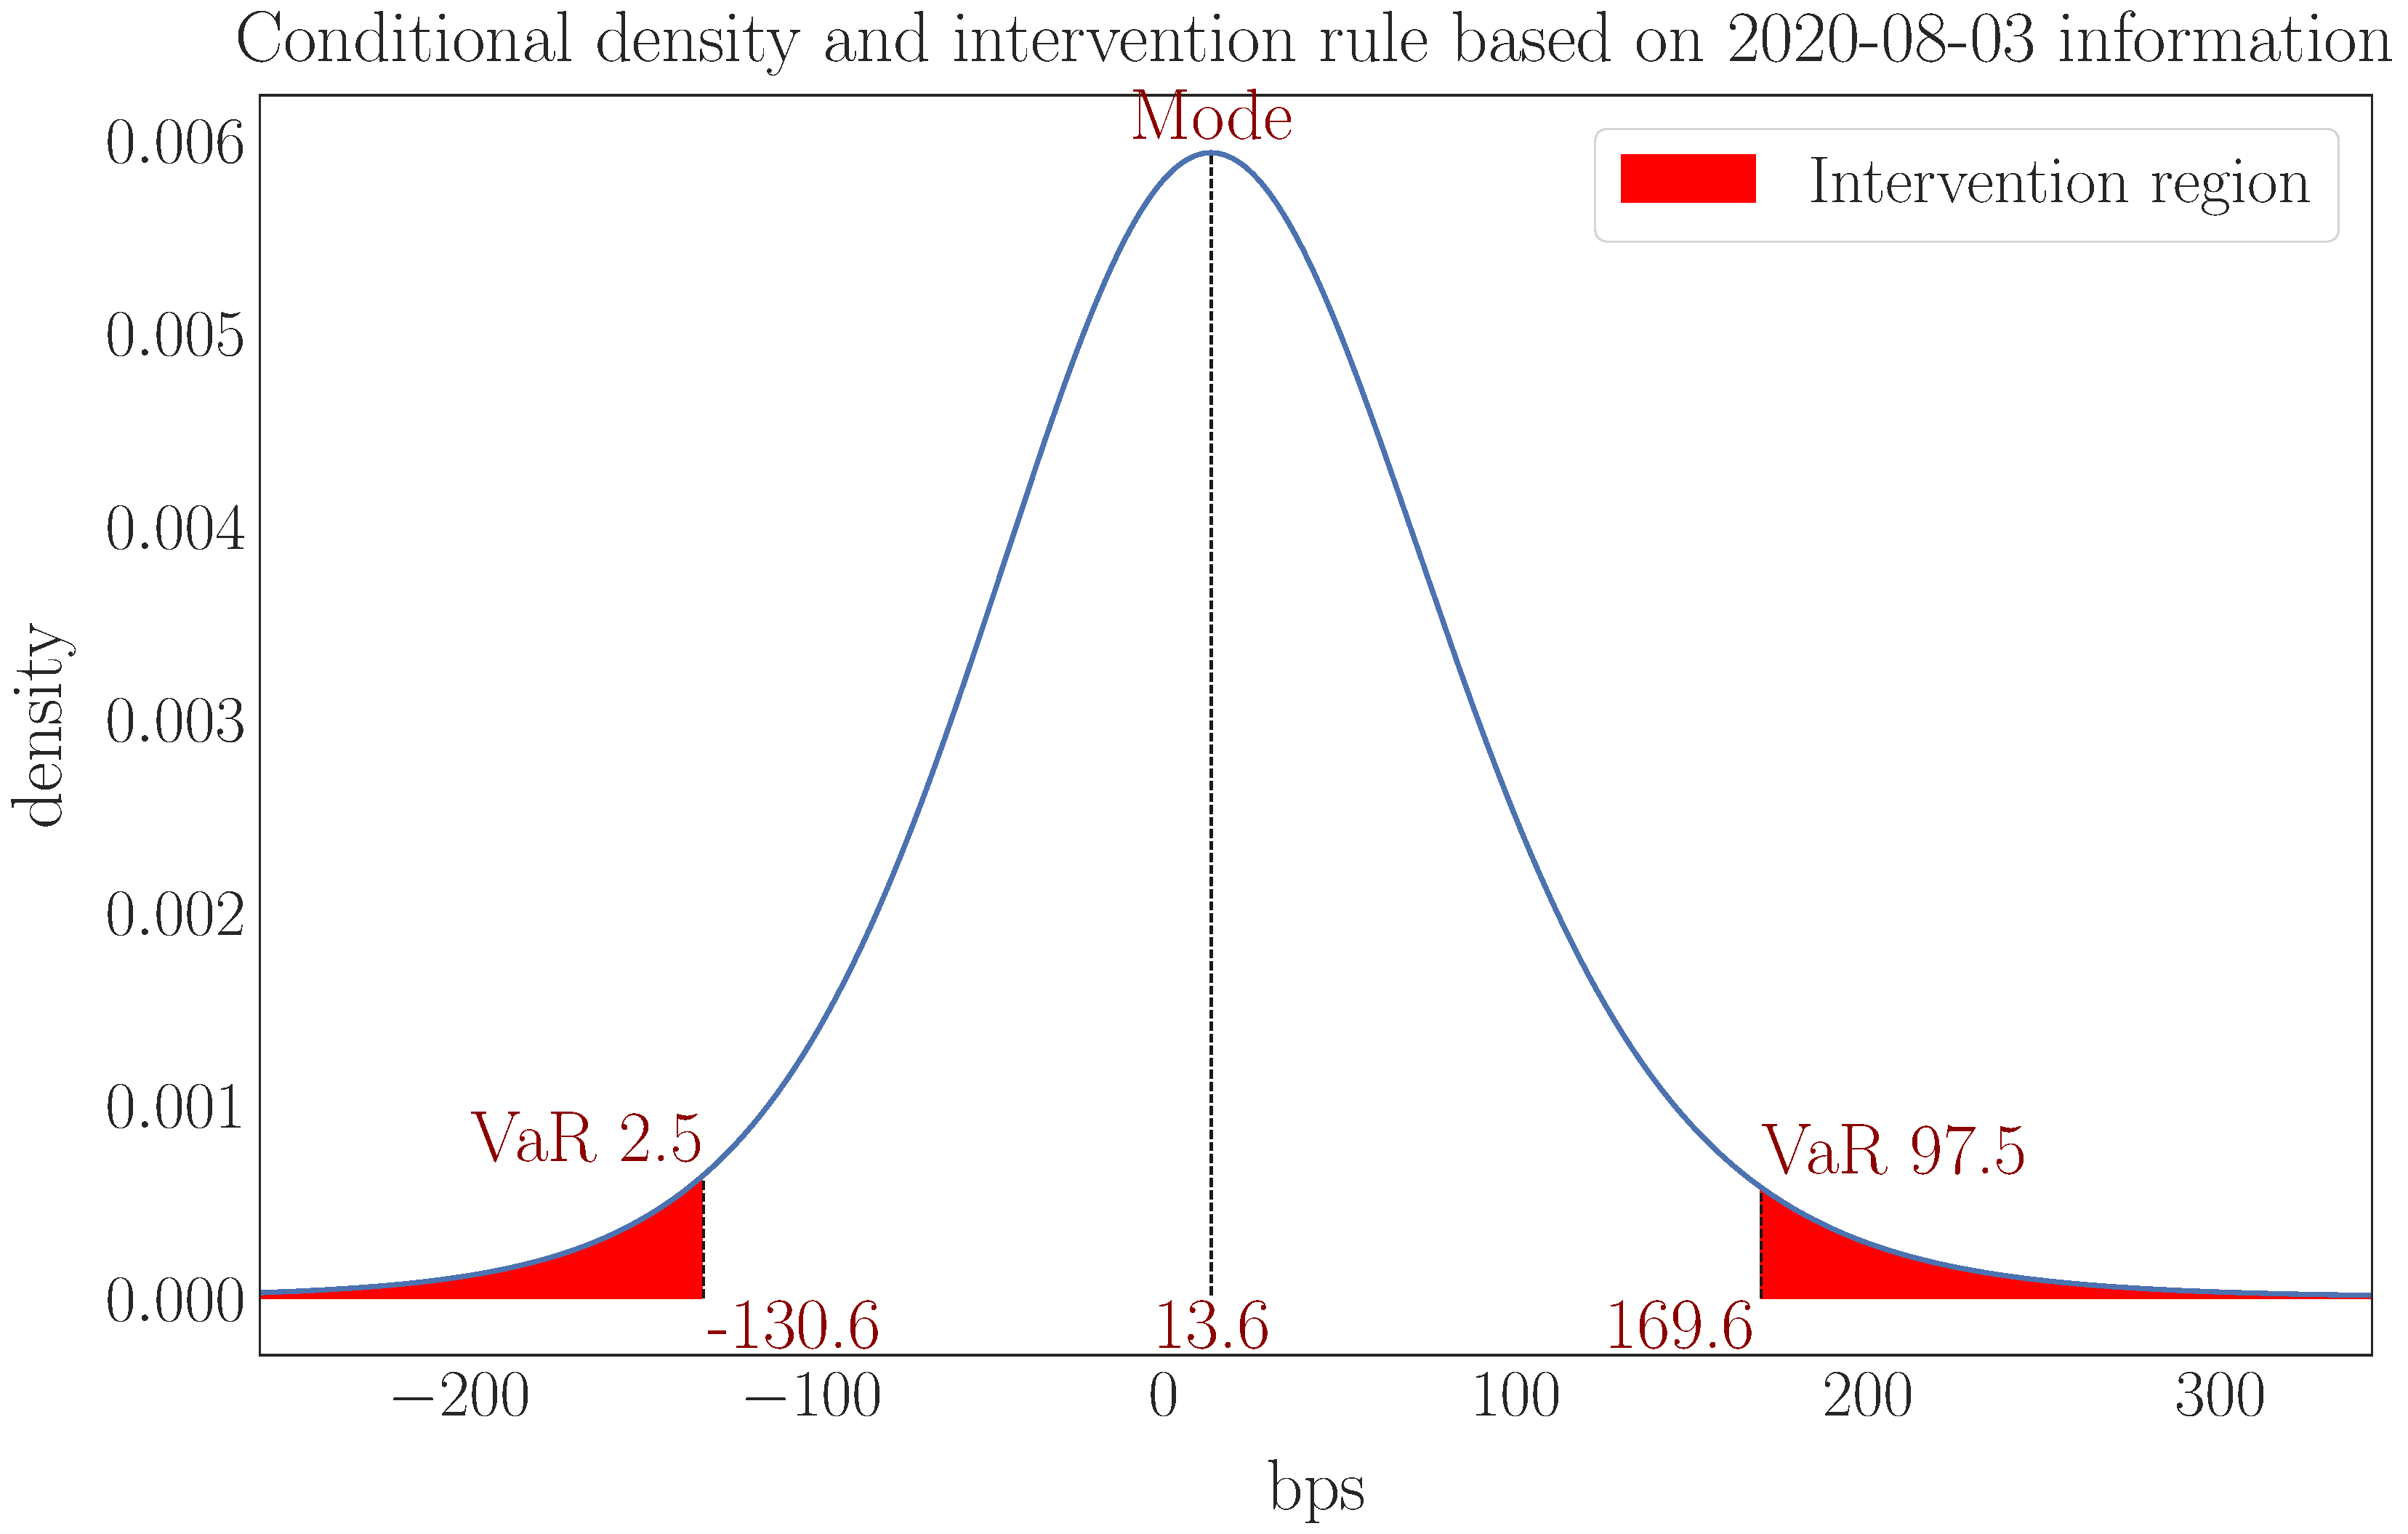
\includegraphics[width= 0.95\textwidth, keepaspectratio]{../output/var_rule.pdf}
\label{fig:var-rule}
\source{\emph{Sources}: authors' calculations}
\end{figure}


Over  time, the  VaR-FXI  rule can  be  represented by  the  region where  the
cumulative  distribution   function  falls  outside  the   central  bank  risk
tolerance,  for example,  the 2.5th  and 97.5th  percentiles, as  presented in
Figure \ref{fig:conditional-cdf}.\\

\begin{figure}
  \centering
  \caption{Conditional Cumulative Distribution Function and Intervention Thresholds}
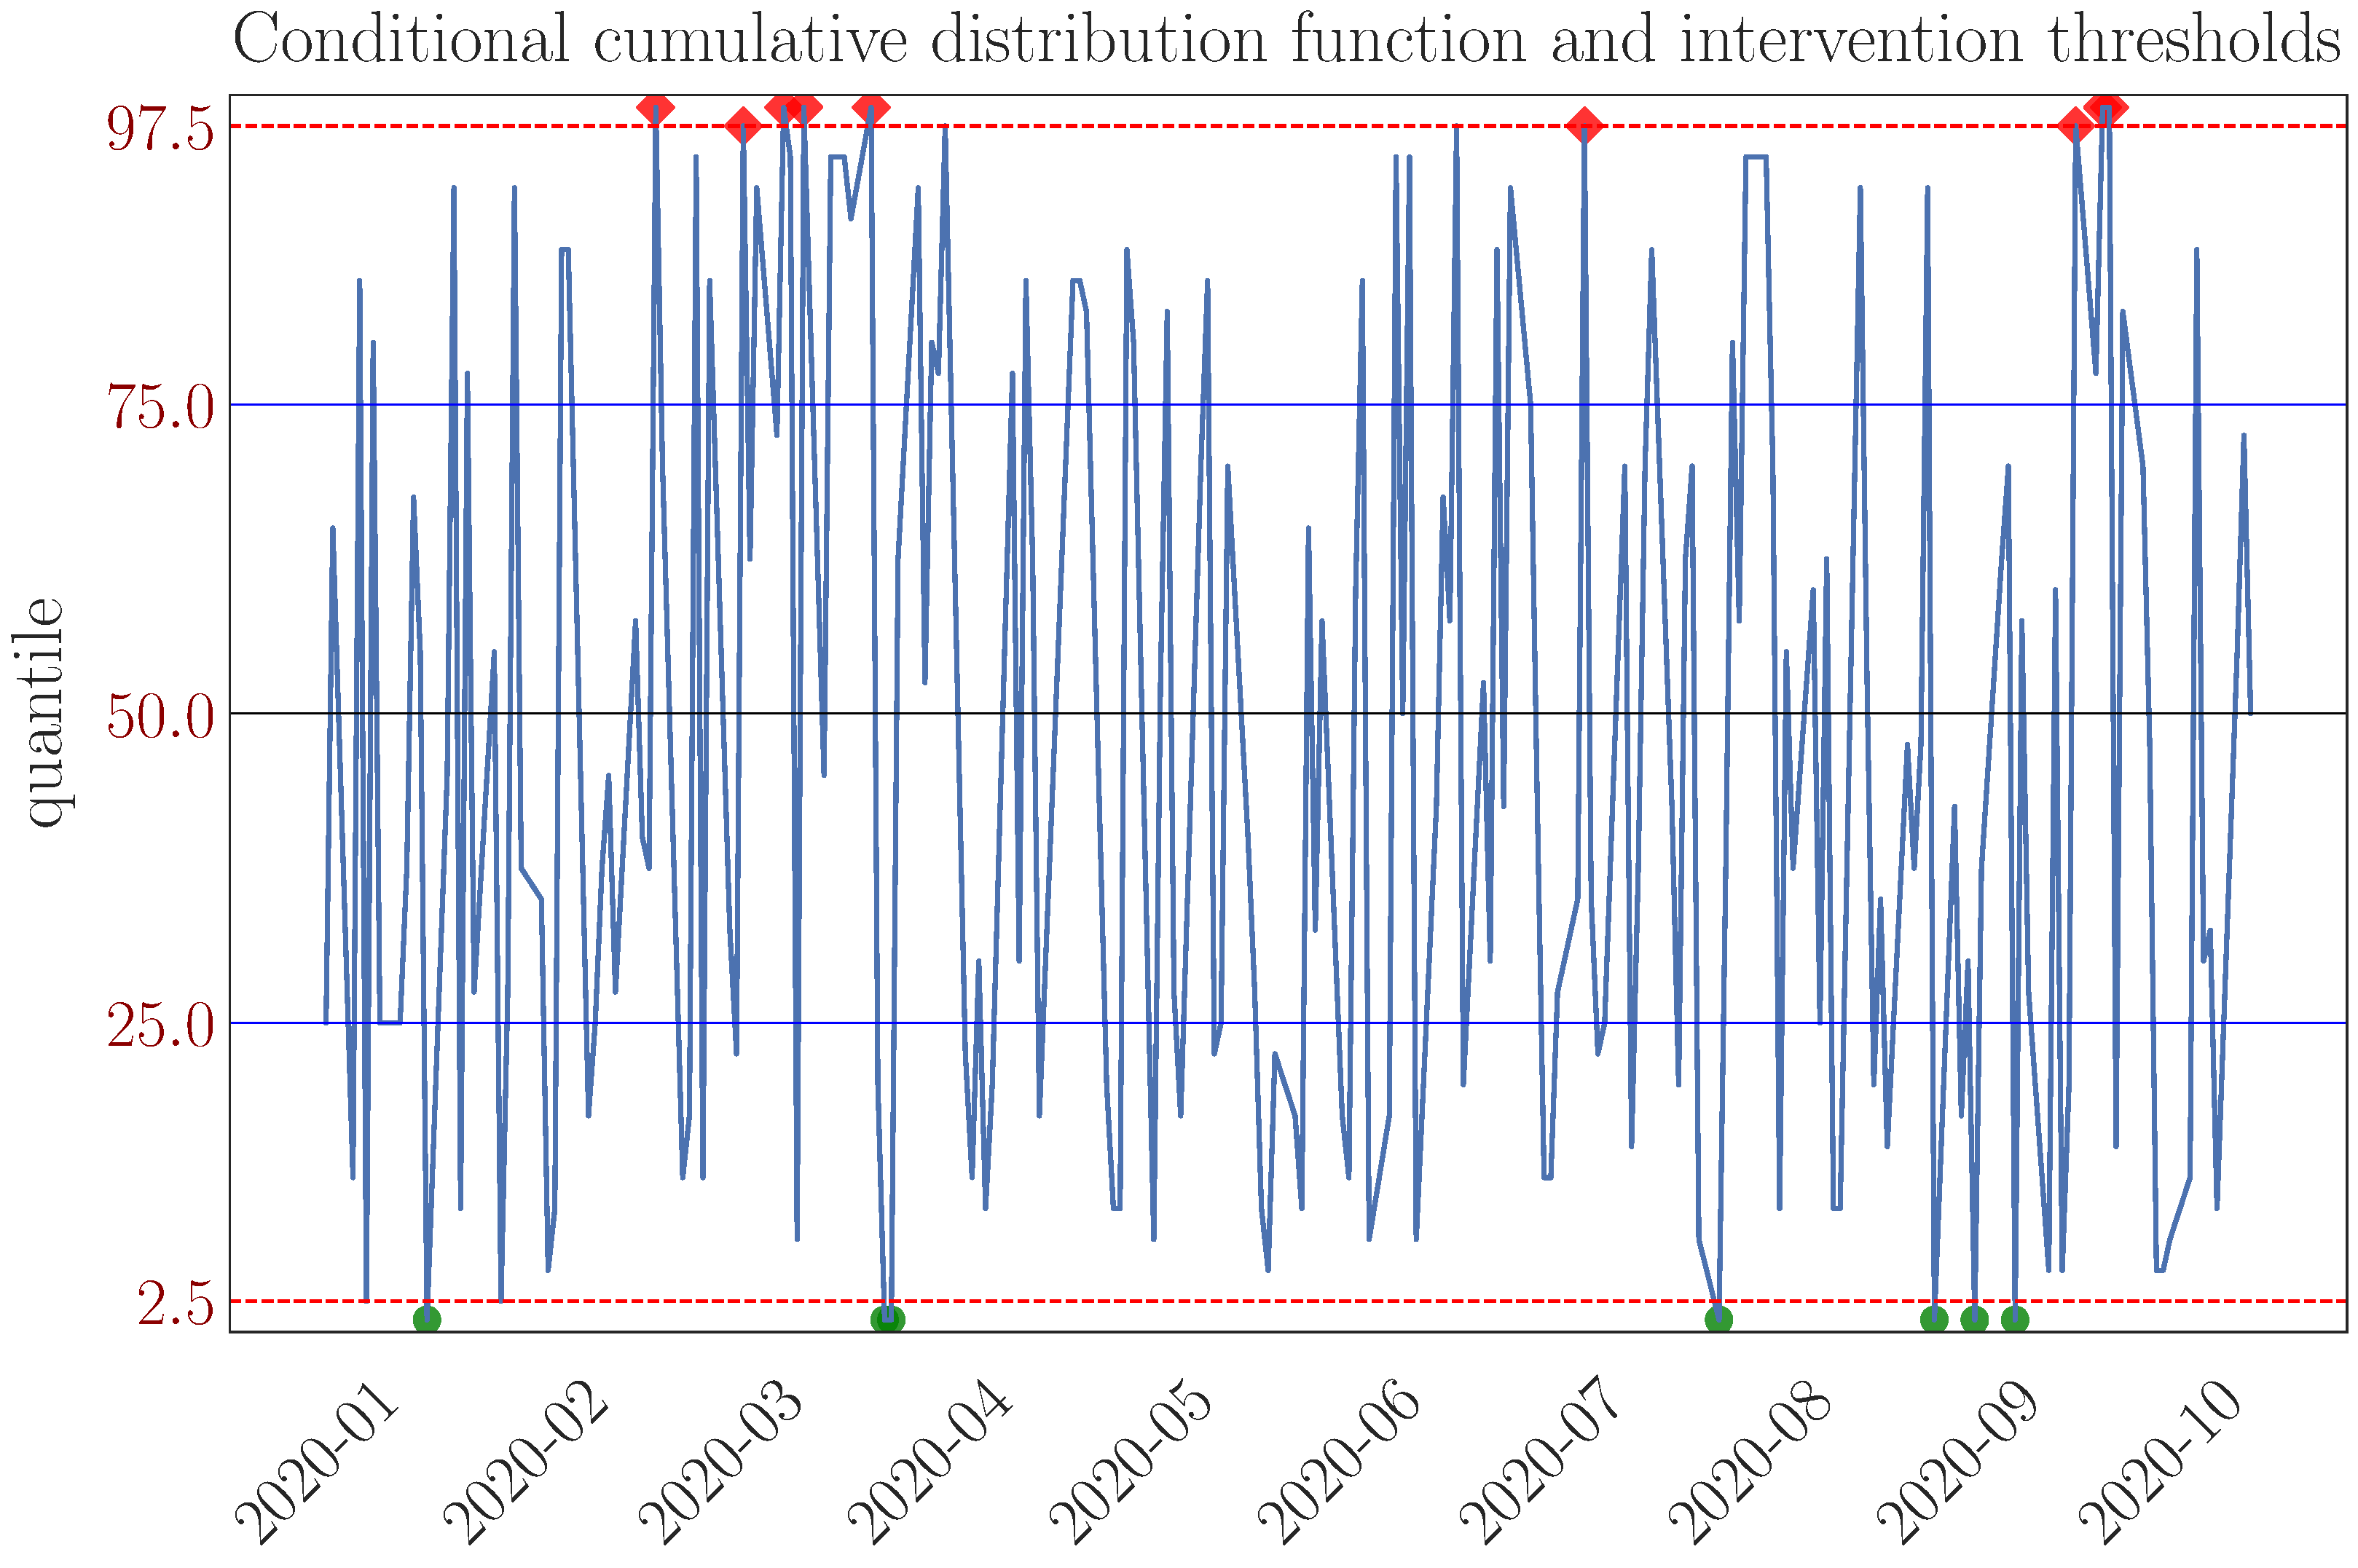
\includegraphics[width= 0.95\textwidth, keepaspectratio]{../output/conditional_cdf.pdf}
\label{fig:conditional-cdf}
\source{\emph{Sources}: authors' calculations}
\end{figure}


Had the BM followed the VaR FX  intervention rule, it might have intervened in
about 15  days over  10 months,  from January through  October 2020.  Figure 9
presents  the  intervention  days  within   the  daily  log-returns  plot.  It
highlights with green  dots (below ERaR 2.5th percentile) and  red dots (above
the  ERaR  97.5th percentile)  the  occurrences  falling in  the  intervention
regions. The  lower chart  presents the  corresponding FX  level in  which the
central bank would have intervened. Fifteen days of intervention correspond to
about 7.5 percent of  the period, even when using an  intervention region of 5
percent.  The frequency  of interventions  would increase  when volatility  is
unusually high, which  was the case during the COVID-19  crisis. However, this
exercise is  purely counterfactual, and it  is likely that after  the first FX
intervention, the FX volatility would  have decreased, hence reducing the need
for future interventions.\\

\begin{figure}
  \centering
  \caption{Conditional VaR Exceedance, Out-of-Sample}
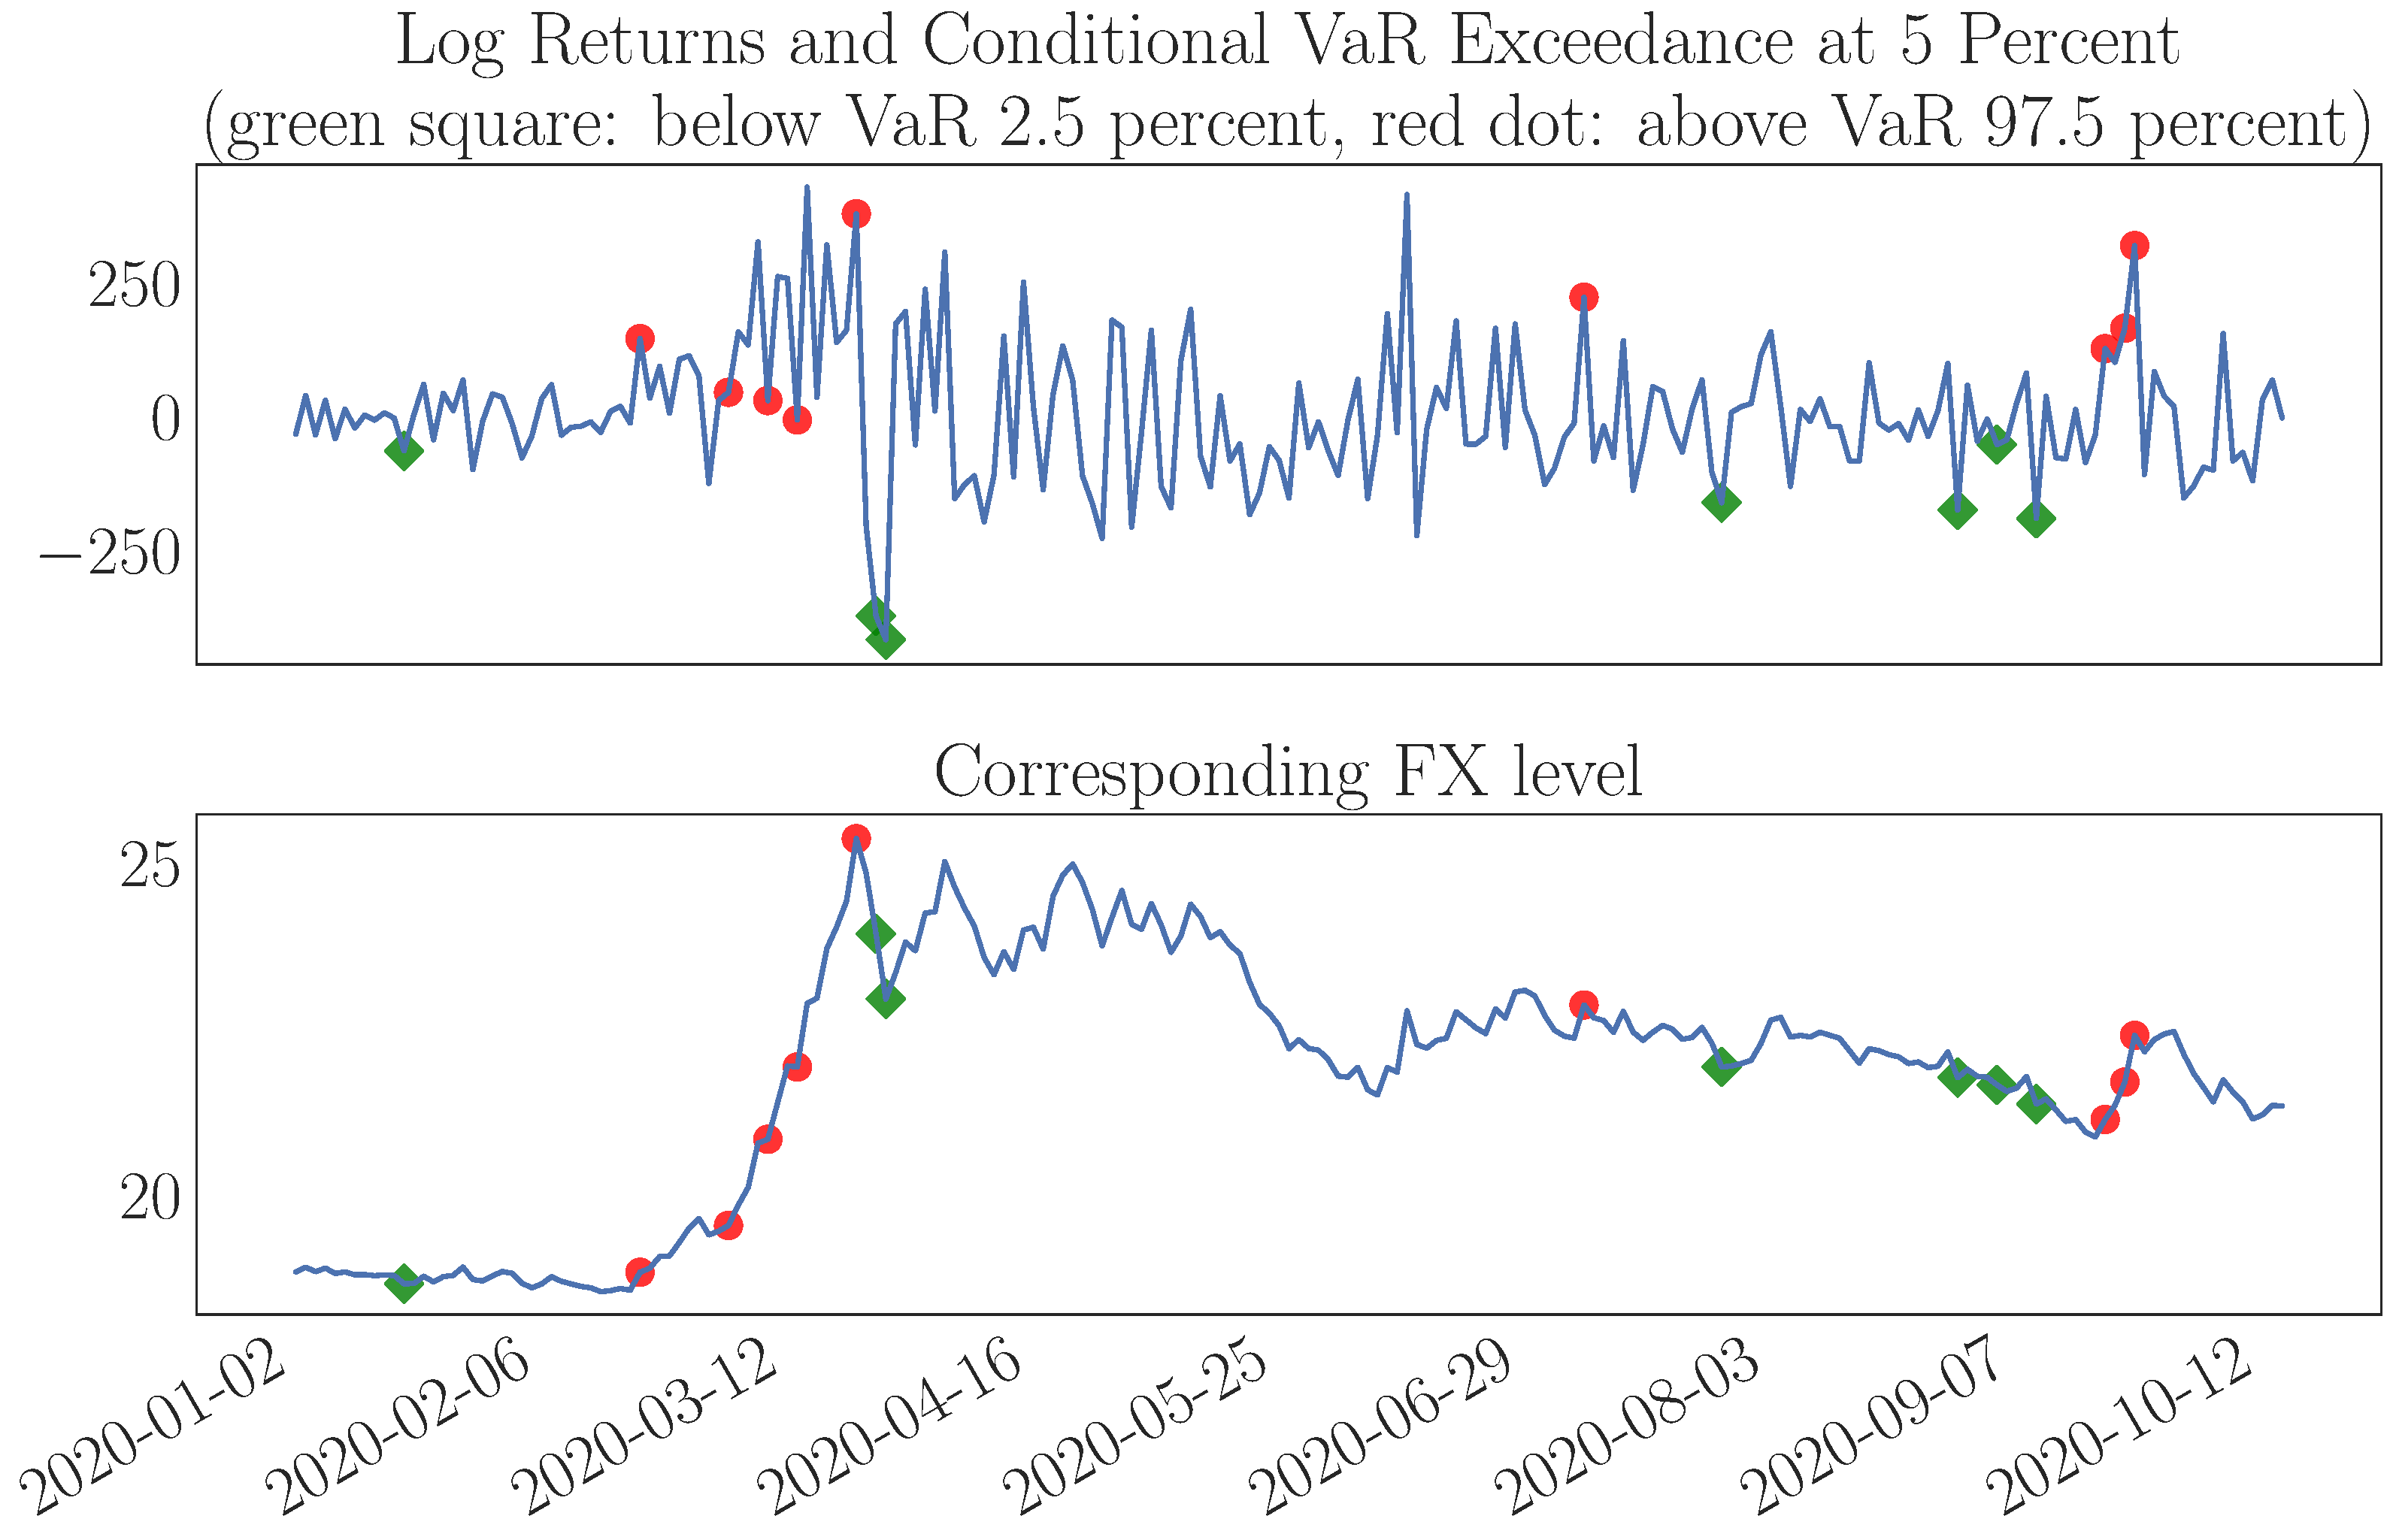
\includegraphics[width= 0.95\textwidth, keepaspectratio]{../output/conditional_exceedance.pdf}
\label{fig:conditional-exceedance}
\source{\emph{Sources}: authors' calculations}
\end{figure}


\subsection{FX Intervention Calibration under Risk-Based Interventions}
\label{sec:calibration}

One of the major  advantages of the VaR FX rule is  that it provides certainty
about the  frequency of FX interventions  over time. For example,  with a risk
tolerance of 2.5  percent both for depreciation and  appreciation, the central
bank will, on average, intervene 5 percent of the time. The central bank might
temporarily  deviate  over   a  short  period  of   time―depending  on  market
conditions―but  the VaR  approach  guarantees that  over  a sufficiently  long
period of time, the frequency is the same as the risk tolerance.\\

Another substantial benefit of  the VaR rule is that it can  be designed to be
budget neutral for  the central bank over the medium  term. Should the central
bank decide  to operate  with a  symmetric rule (the  same risk  tolerance for
appreciation and depreciation), it will intervene  the same number of times on
both sides, hence offsetting selling FX with buying FX.\\

Over the  short term, the  central bank may temporarily  sell more FX  than it
buys, depending on  market conditions. The fixed-frequency feature  of the VaR
can, therefore,  be used  to determine  the budget  constraint of  the central
bank,  that is,  that the  central  bank has  enough reserves  to conduct  the
interventions  in   a  credible   and  efficient   way.  A   conservative  and
straightforward approach  is to  make sure  that the  maximum amount  of daily
intervention times the frequency on the depreciation side (the risk tolerance)
is always  less than the  amount of  FX reserves the  central bank has  for FX
interventions. The  maximum amount of  daily intervention should be  enough to
have an  impact on  the exchange  rate when the  central bank  intervenes, for
example, by making sure it represents a significant share of the average daily
market turnover across time.\\


%% ---------------------------------------------------------------------------
%% The Case of Mexico
%% ---------------------------------------------------------------------------

\section{The Case of Mexico}
\label{sec:mexico-case}

The Banco  Mexico intervened via two  types of auctions whose  main difference
was the reservation  rate applied to each  auction. In the first  type, the BM
operated an auction  every day with a preannounced reservation  rate, that is,
the  minimum rate  for eligible  bids. The  auction with  a minimum  price was
suspended in  April 2010 and  reintroduced with  changes in November  2011 and
suspended         again         after         April         2013.\footnote{See
\url{https://www.banxico.org.mx/markets/auctions-with-minimum-price-e.html for
more  details}} On  many  days, the  rule-based auction  did  not receive  any
demand, as the market was operating  below the reservation rate. In the second
type, the  auction was organized  when the BM found  it opportune and  did not
have a reservation rate (an auction  without a minimum rate). For some periods
(for example,  during 2015), daily  interventions were preannounced  without a
minimum price. Size was also preannounced and later adjusted.\\

The BM may have intervened for  more reasons than preventing disorderly market
conditions. The exact  rationale for intervention is outside the  scope of the
paper: we are focusing here on  benchmarking the BM FX interventions against a
risk framework, while recognizing that the  BM could have had other objectives
in mind.  We are not assessing the efficiency, the relevance, or the rationale
of the BM interventions.\\


\subsection{Interventions with a Minimum Price}
\label{sec:min-price}

"Auctions with  a minimum  price" were  triggered 31  times from  October 2008
through November 2016.  The auction reservation  price was set at the previous
day's exchange rate close (MEX/USD) multiplied by 1.02 (for example, 2 percent
depreciation)  from October  9,  2008,  to December  8,  2014,  by 1.015  from
December 9, 2014, to November 23, 2015, and by 1.01 from November 24, 2015, to
January 5, 2017. Auctions with a minimum price were suspended after January 5,
2017. Figure \ref{fig:benchmark-minprice} presents the auctions with a minimum
price in green, with the corresponding FX daily log returns and level.\\

\begin{figure}
  \centering
  \caption{FX Interventions Log Returns with Minimum Price}
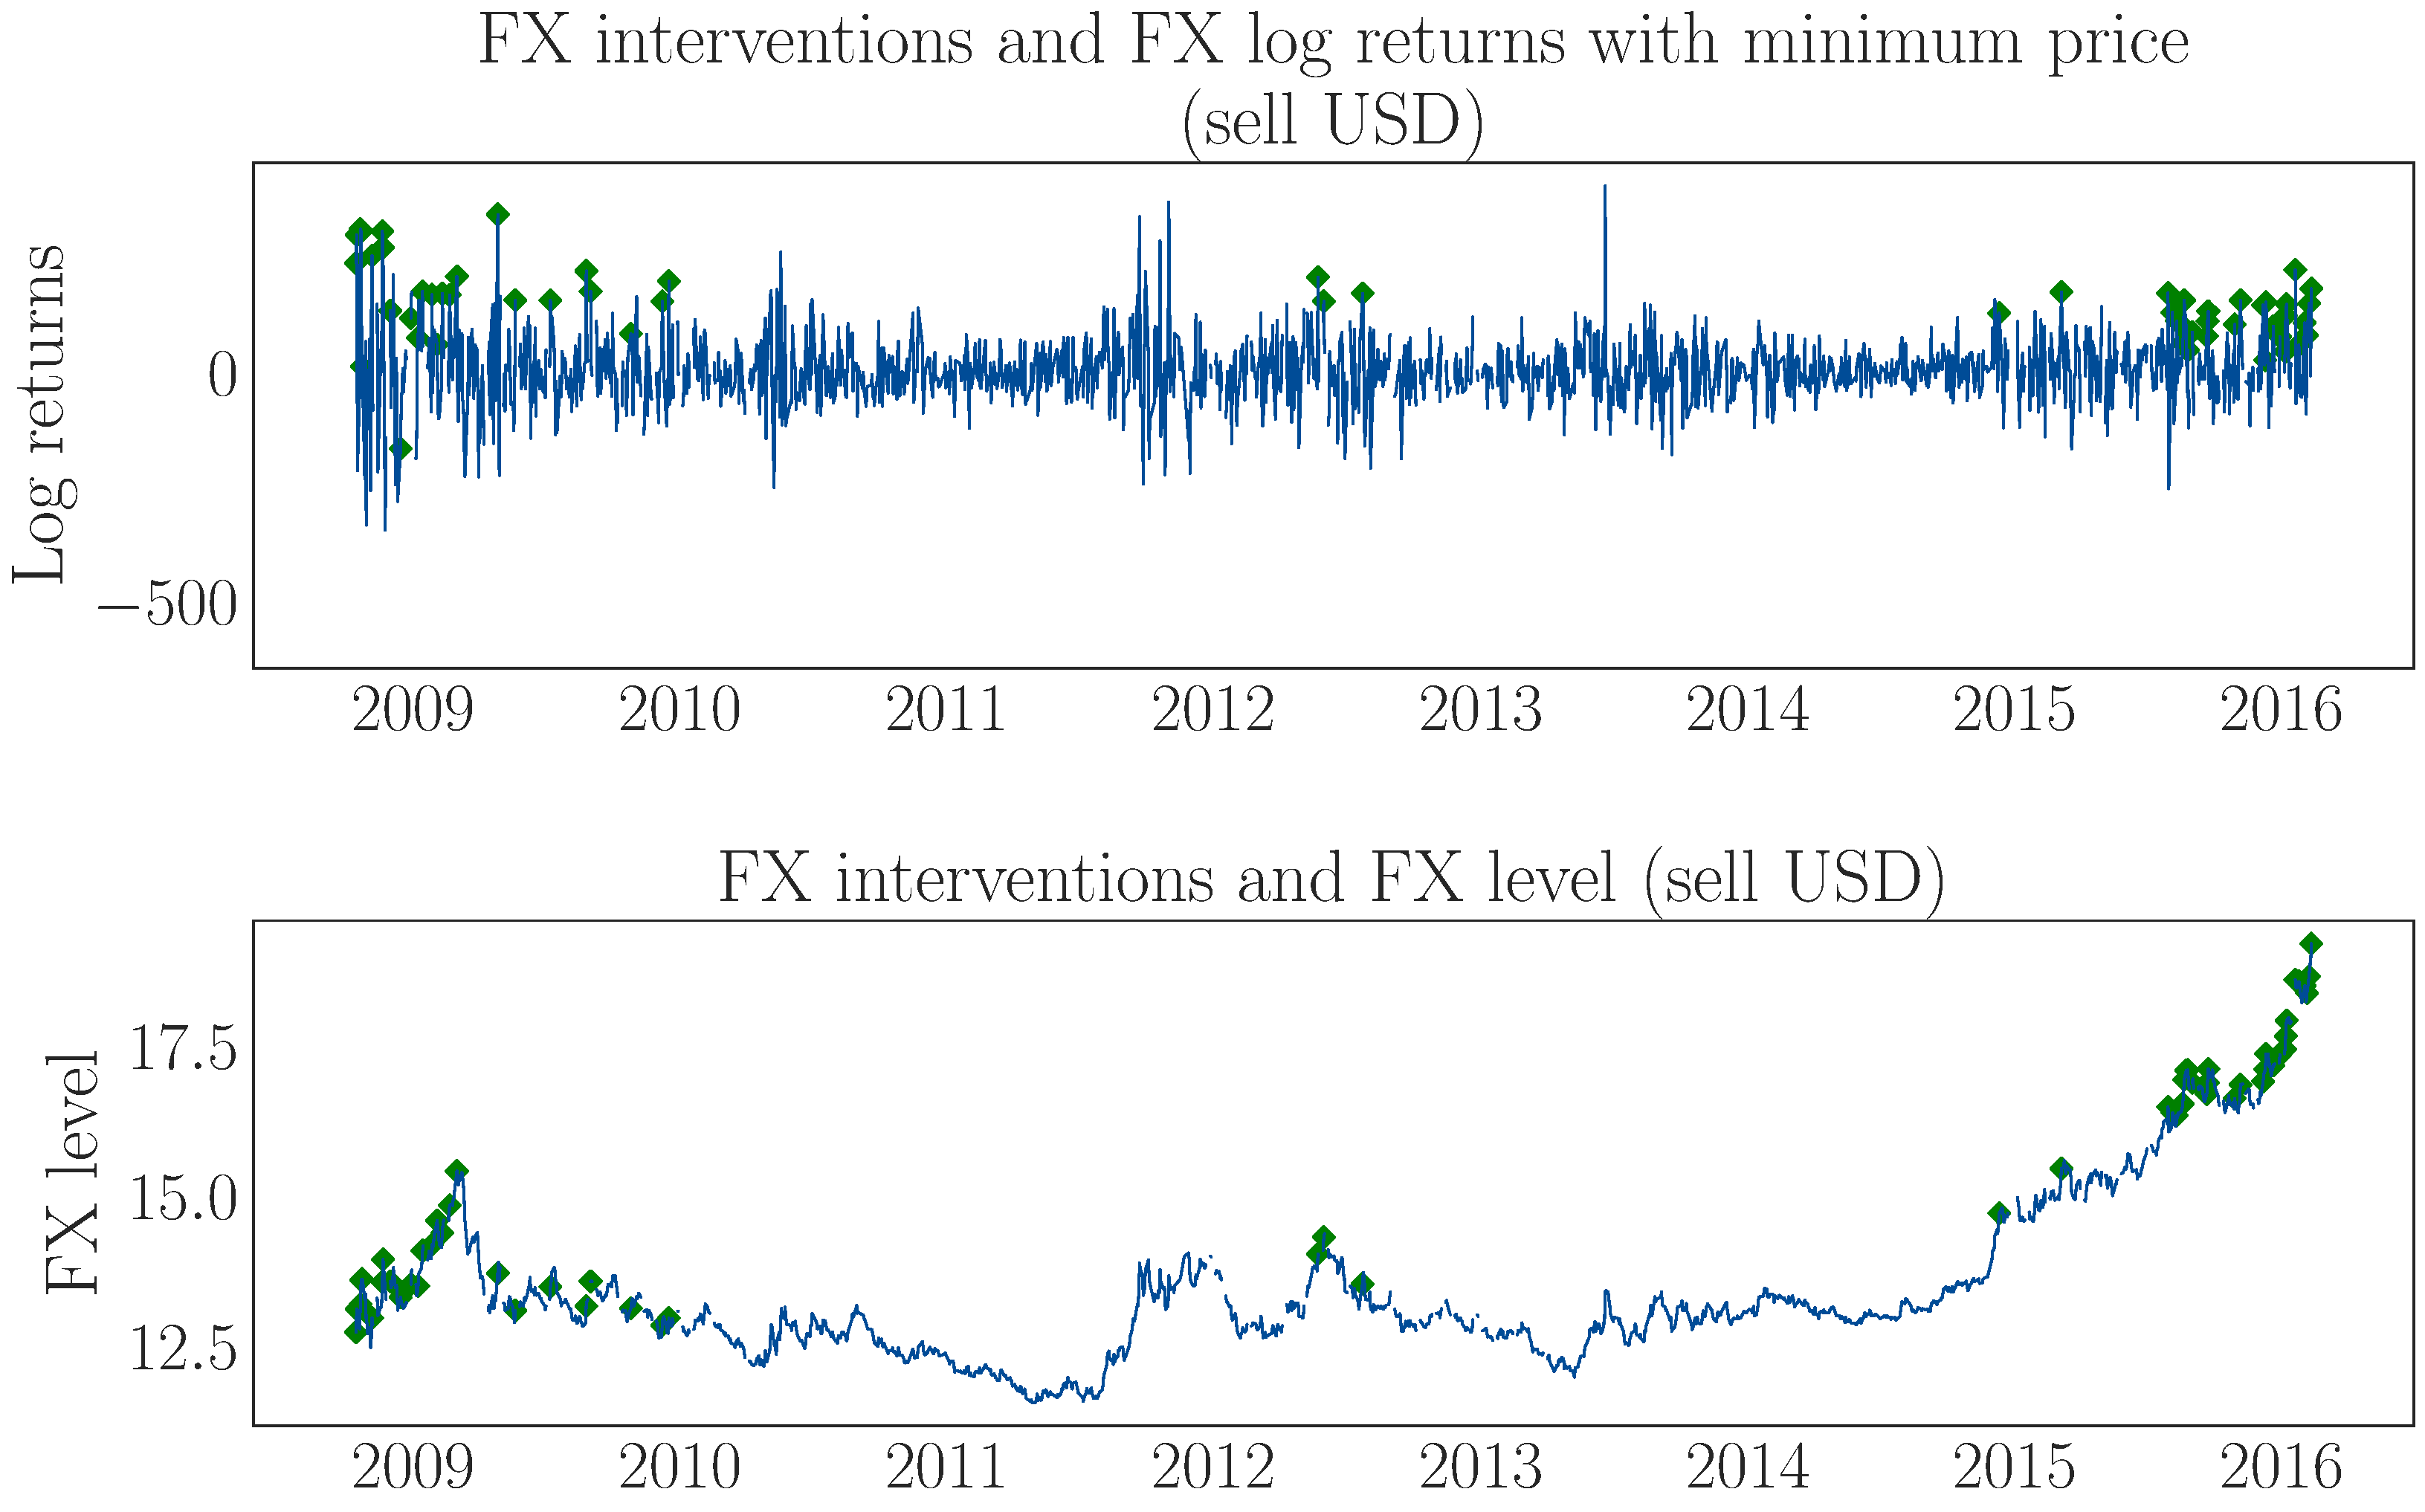
\includegraphics[width= 0.95\textwidth, keepaspectratio]{../output/benchmark_minprice.pdf}
\label{fig:benchmark-minprice}
\source{\emph{Sources}: Banco Mexico and authors' calculations}
\end{figure}

The  VaR  framework can  be  used  by  central  banks to  inform  intervention
decisions, as well  as by external observers to assess  central bank tolerance
for exchange rate risk. First, the framework can be used to assess whether the
central bank responded to exchange rate  volatility and the degree to which it
was  tolerated. Second,  the  framework  can be  used  to  assess whether  the
interventions efficiently achieved the authorities' objectives.\\

The ex-ante  conditional cumulative distribution function  (CDF) estimated via
the   GARCH   model    is   used   to   benchmark   the    Banco   Mexico   FX
interventions. Although the  central bank did not use the  model to intervene,
one can always assess the corresponding  FX rate conditional quantile when the
central   bank  has   intervened.   The   outcome  is   presented  in   Figure
\ref{fig:benchmark-minprice-cdf}.  The  back-testing exercise shows  that most
FX   interventions   have   occurred   on   the   top   of   the   conditional
distribution―where the depreciation  was the largest―and often  above the 95th
percentile. A few outliers  occur at the median or below,  but these cases are
rare. Overall,  the interventions with  the minimum price approach  were often
but not  always equivalent to  a risk  framework: the central  bank intervened
most of the time when the pressure  on the exchange rate was the largest, with
exceptions.\\

\begin{figure}
  \centering
  \caption{Conditional CDF of FX Intervention with Minimum Price}
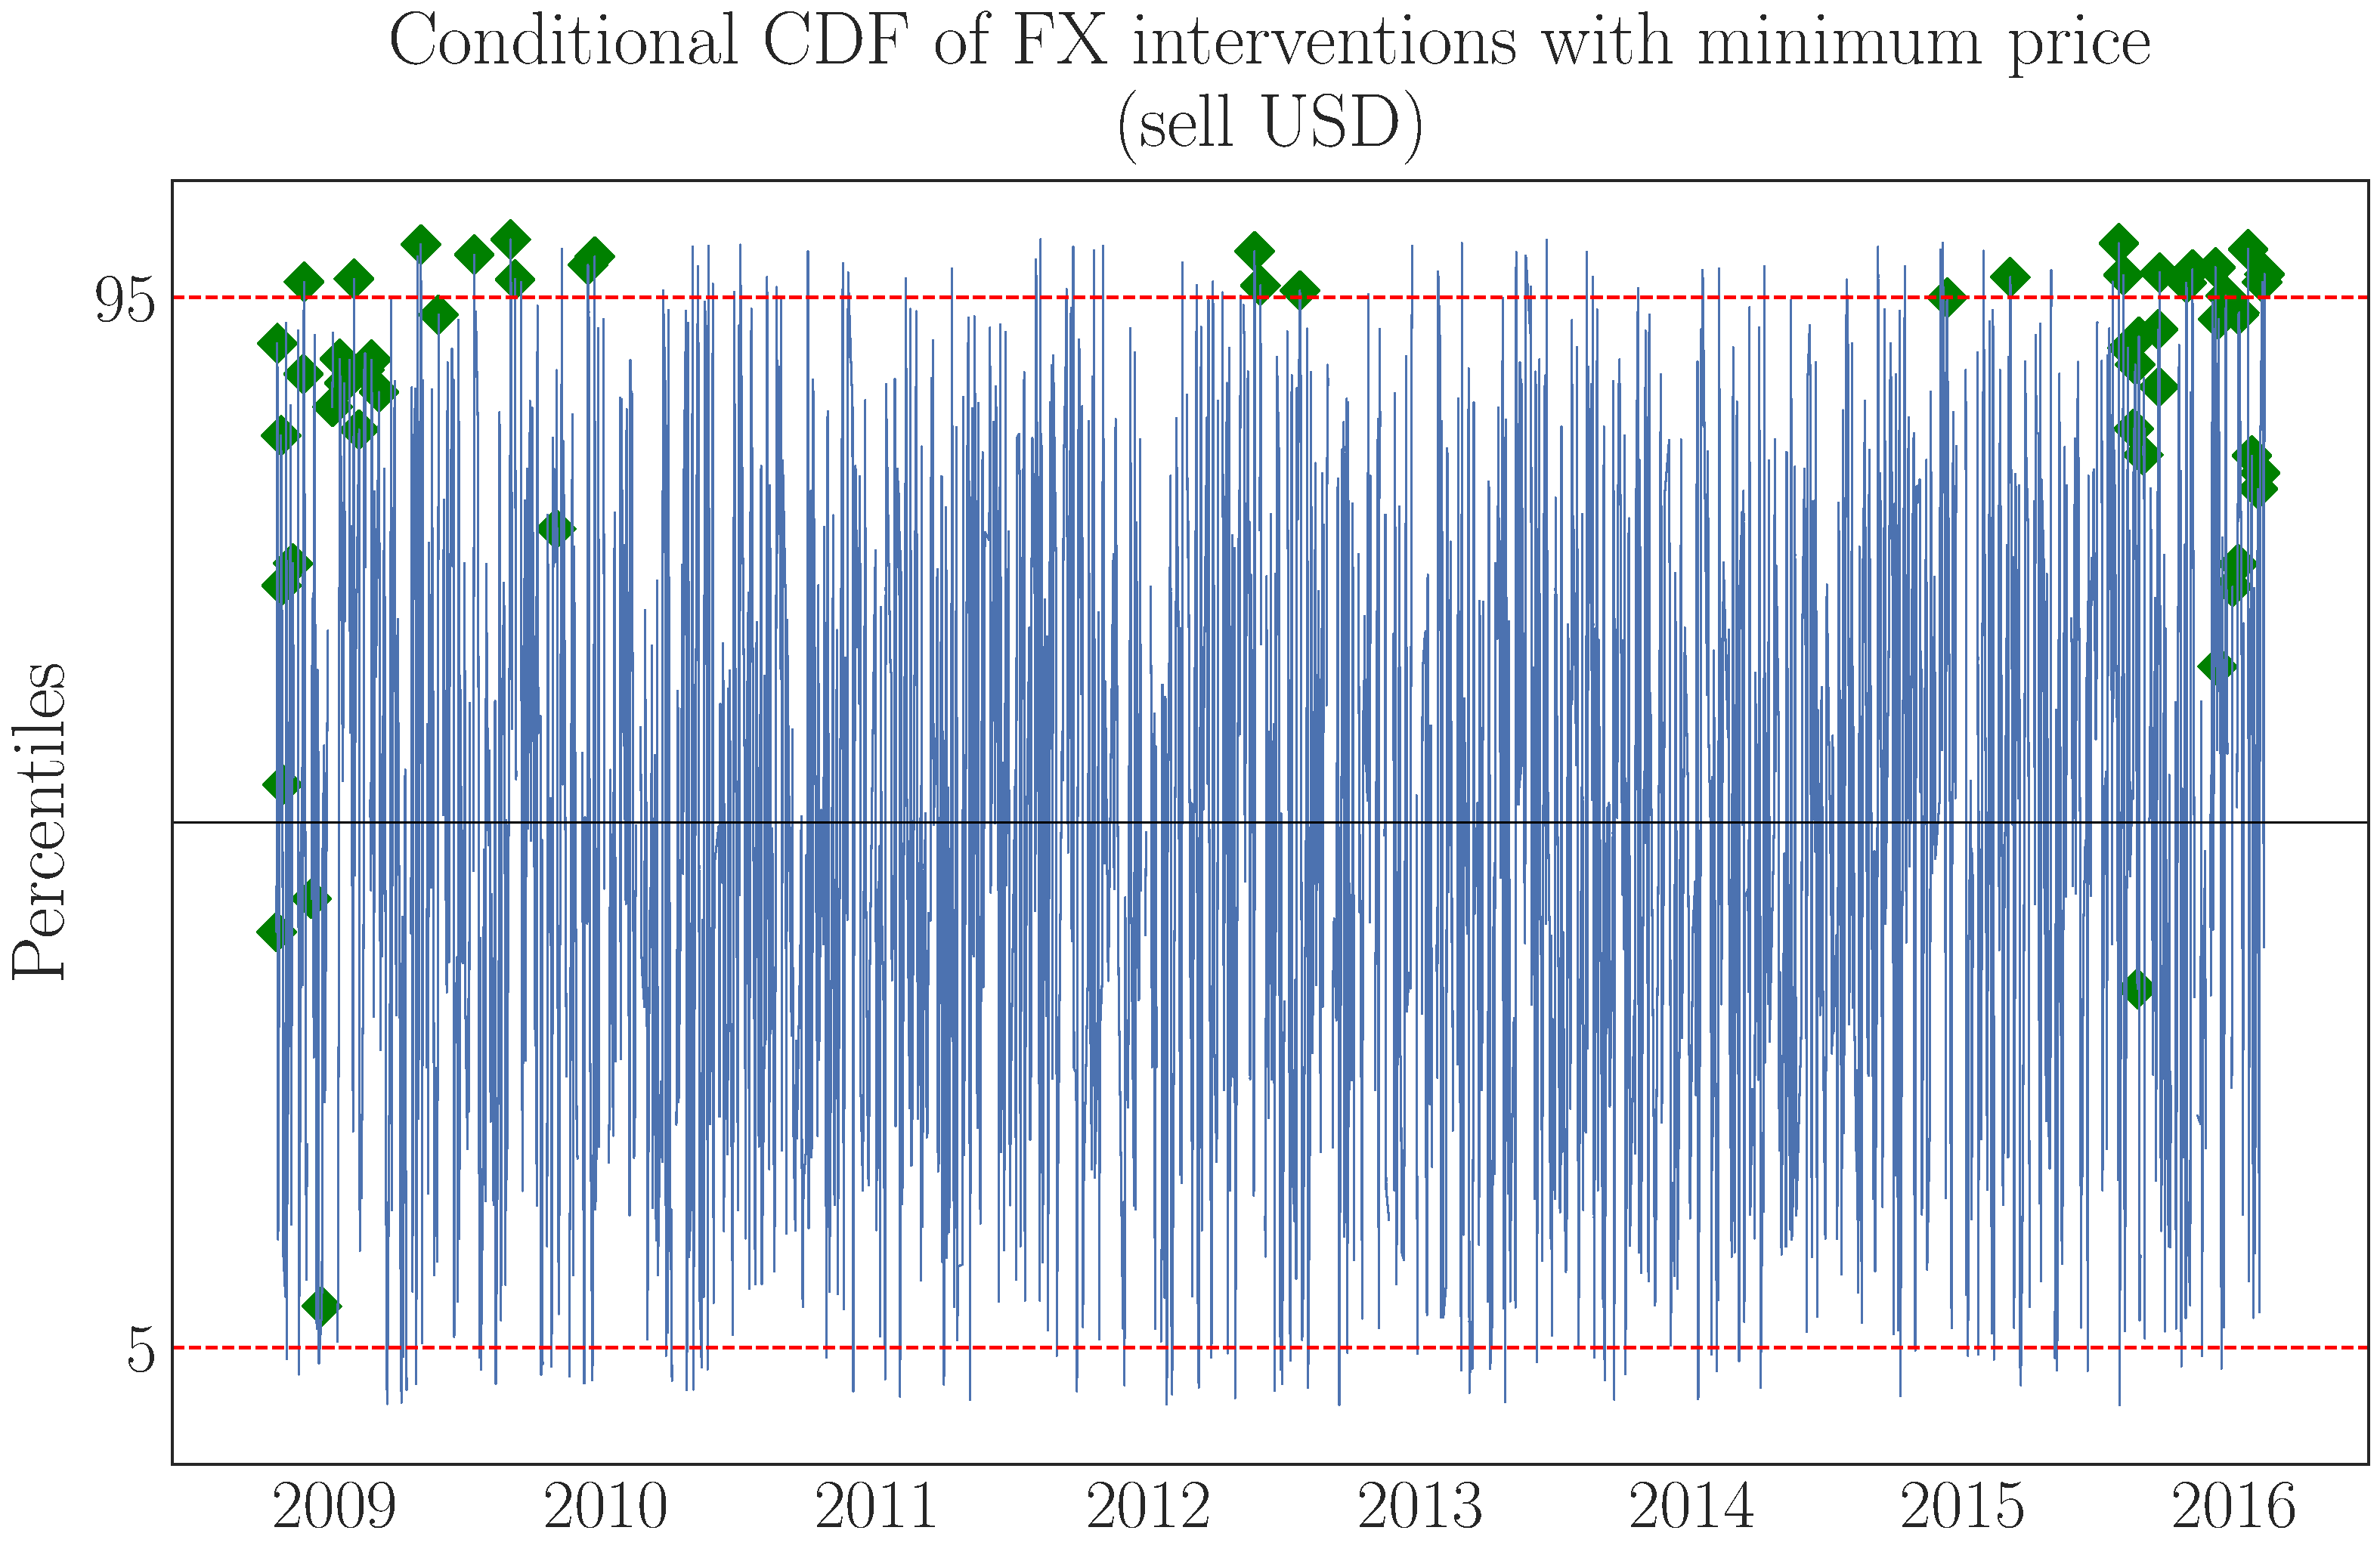
\includegraphics[width= 0.95\textwidth, keepaspectratio]{../output/benchmark_minprice_cdf.pdf}
\label{fig:benchmark-minprice-cdf}
\source{\emph{Sources}: Banco Mexico and authors' calculations}
\end{figure}


\subsection{Interventions without a Minimum Price}
\label{sec:nomin-price}

The BM  organized 319 "auctions without  a minimum price" from  September 2009
through November 2015.  Interventions without  a minimum price overlapped with
"auctions  with  a  minimum  price,"  which  could  constrain  the  volatility
distribution even  in the  absence of actual  intervention under  the rule―the
mere presence  of the  rule influences  market participants'  behavior. Figure
\ref{fig:benchmark-nominprice} presents the FX interventions without a minimum
price on the Mexican pesos in red, with the corresponding FX daily log returns
and level.\\

\begin{figure}
  \centering
  \caption{FX Interventions without a Minimum Price on the Mexican Peso/US Dollar}
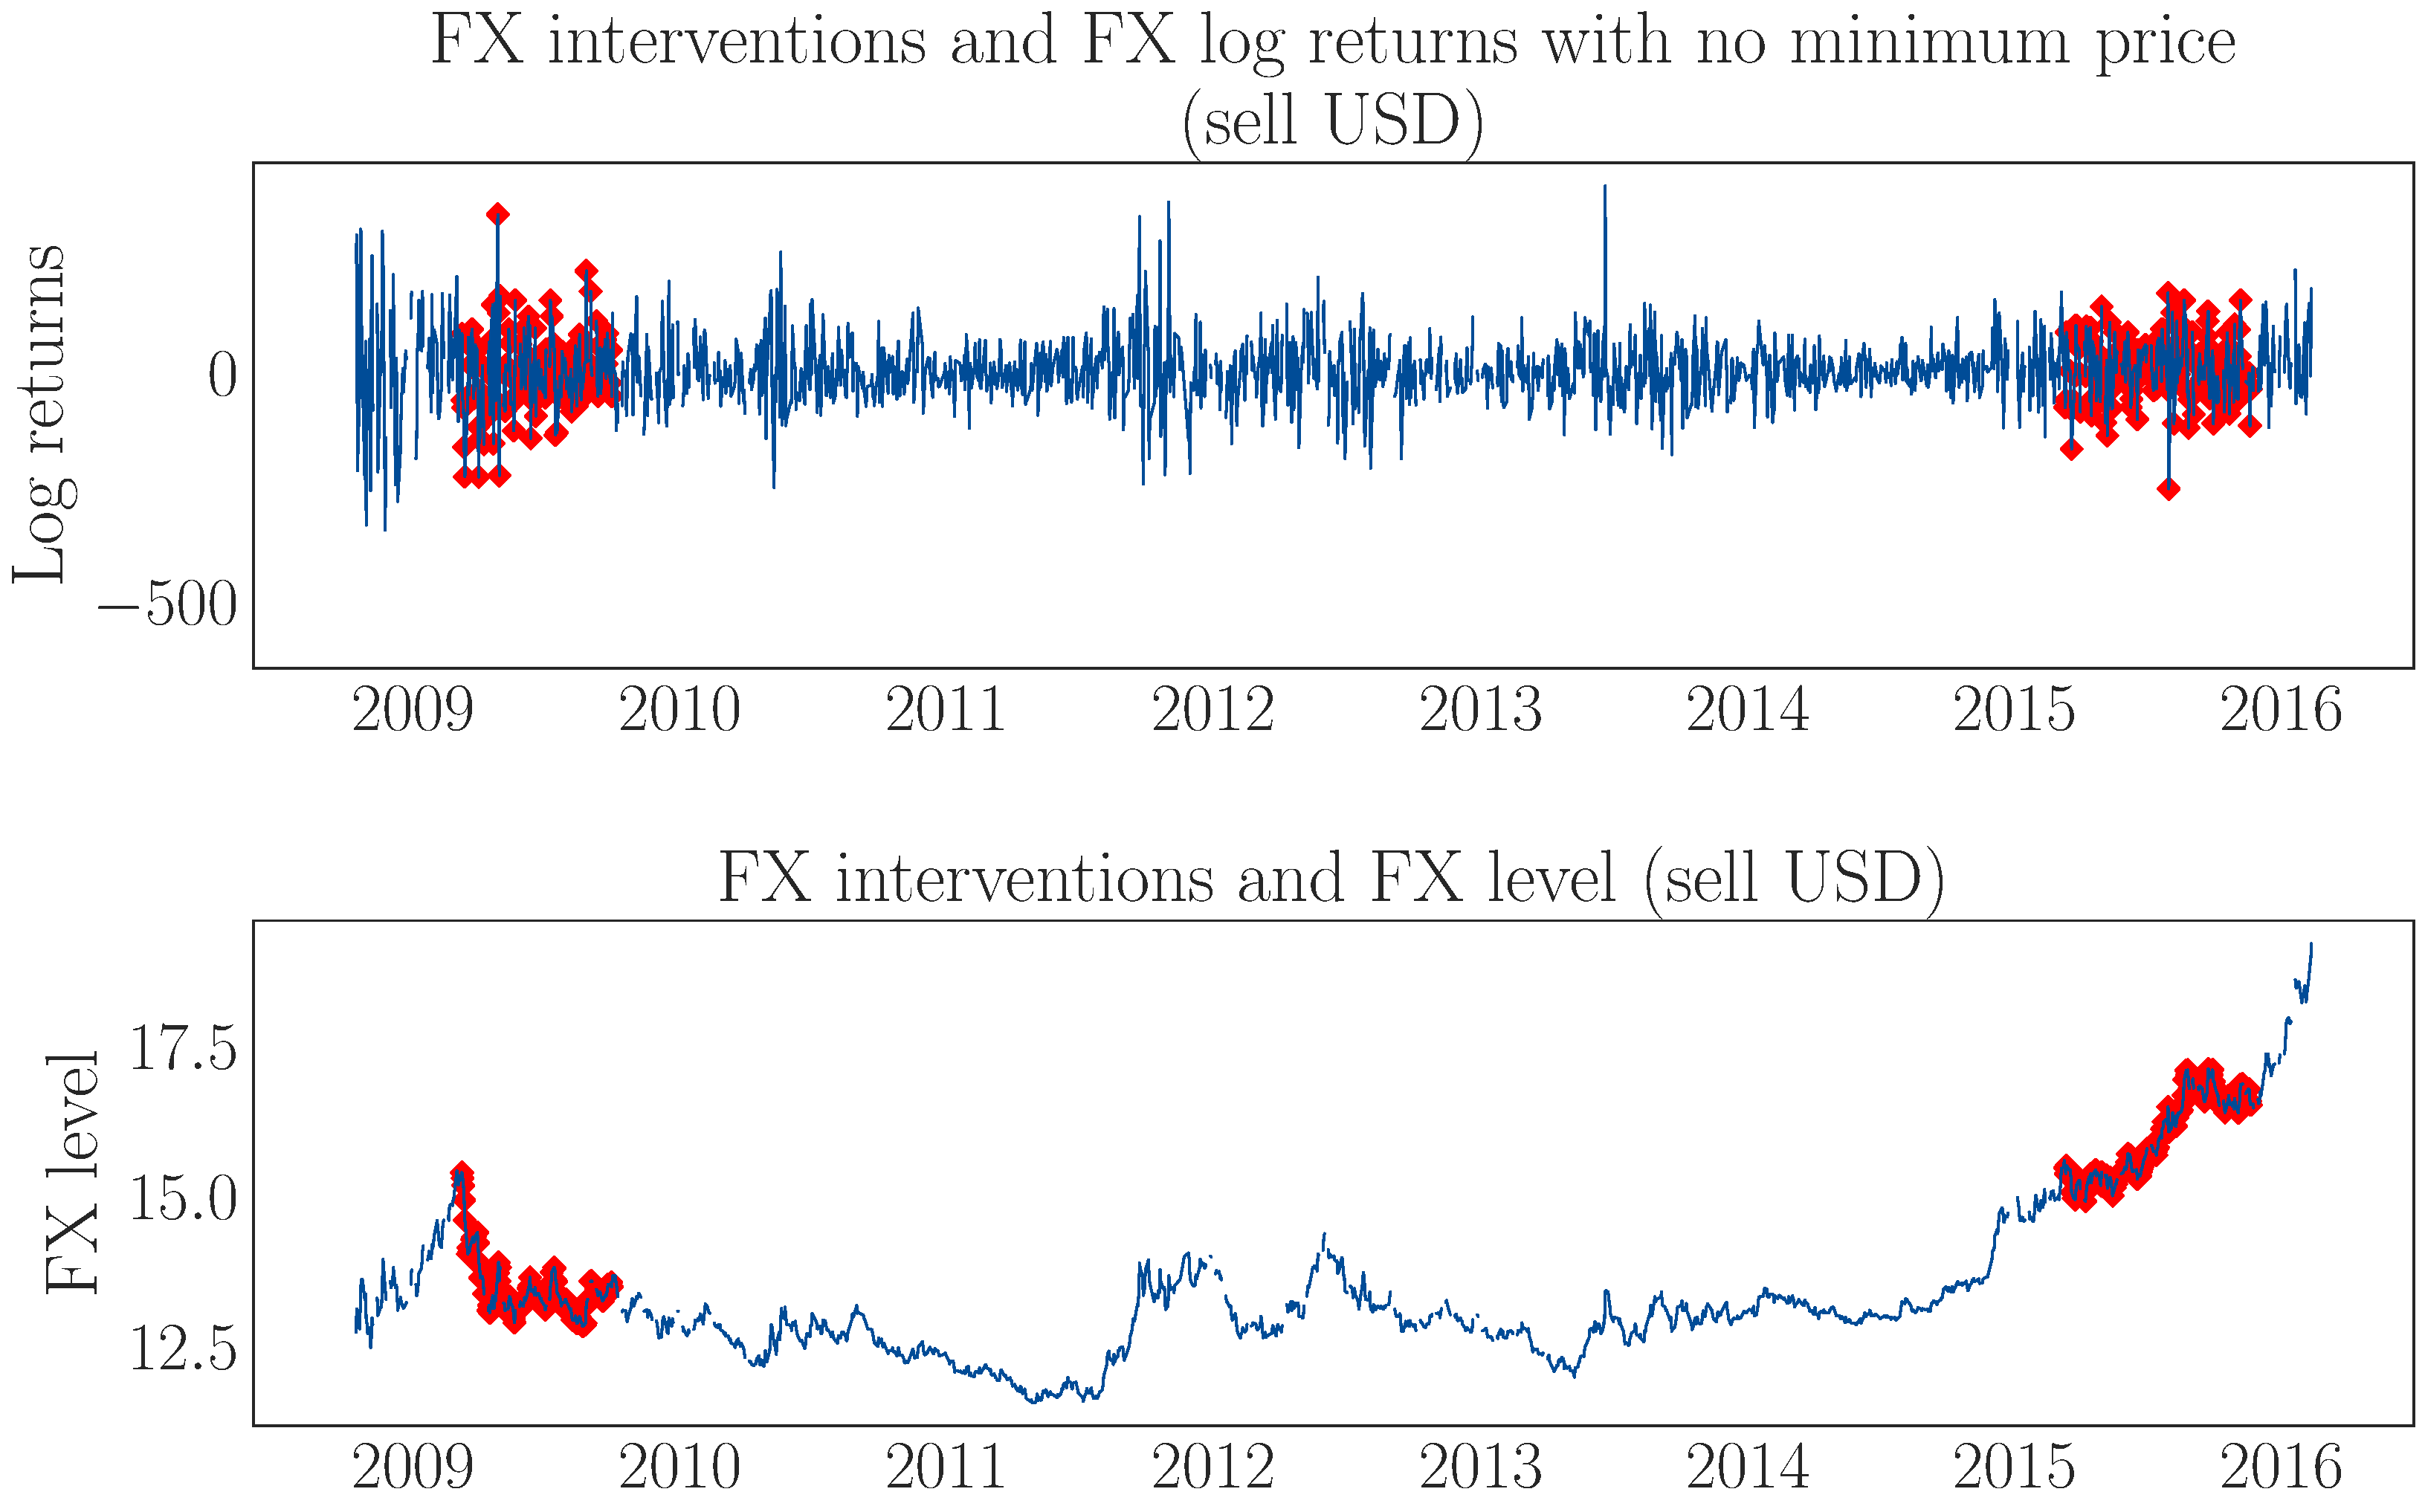
\includegraphics[width= 0.95\textwidth, keepaspectratio]{../output/benchmark_no_minprice.pdf}
\label{fig:benchmark-nominprice}
\source{\emph{Sources}: Banco Mexico and authors' calculations}
\end{figure}


As in the case of interventions with  a minimum price, the conditional CDF can
be used to benchmark the FX interventions  relative to the risk of the day, as
presented  in Figure  \ref{fig:benchmark-nominprice-cdf}. While  interventions
with  a  minimum price  exhibited  a  pattern  broadly consistent  with  large
depreciation  pressures on  the  exchange rate,  the  interventions without  a
minimum price  have no clear  risk patterns.  Such interventions  had occurred
across the full conditional distribution, even  when the pressures were not on
the depreciation  side but, on the  contrary, the appreciation side.   In this
case, the  fact that the central  bank was selling USD  could have, therefore,
amplified the currency appreciation.  This pattern likely suggests that the BM
rationales  for FX  intervention under  the no-minimum-price  rule are  likely
broader than  just the volatility of  the exchange rate.  For  example, during
certain periods, the motivation for  interventions without a minimum price was
to prevent excessive  accumulation of foreign reserves,  explaining that those
interventions were not related to rate development.\\


\begin{figure}
  \centering
  \caption{FX Interventions without a Minimum Price on the Mexican Peso/US Dollar}
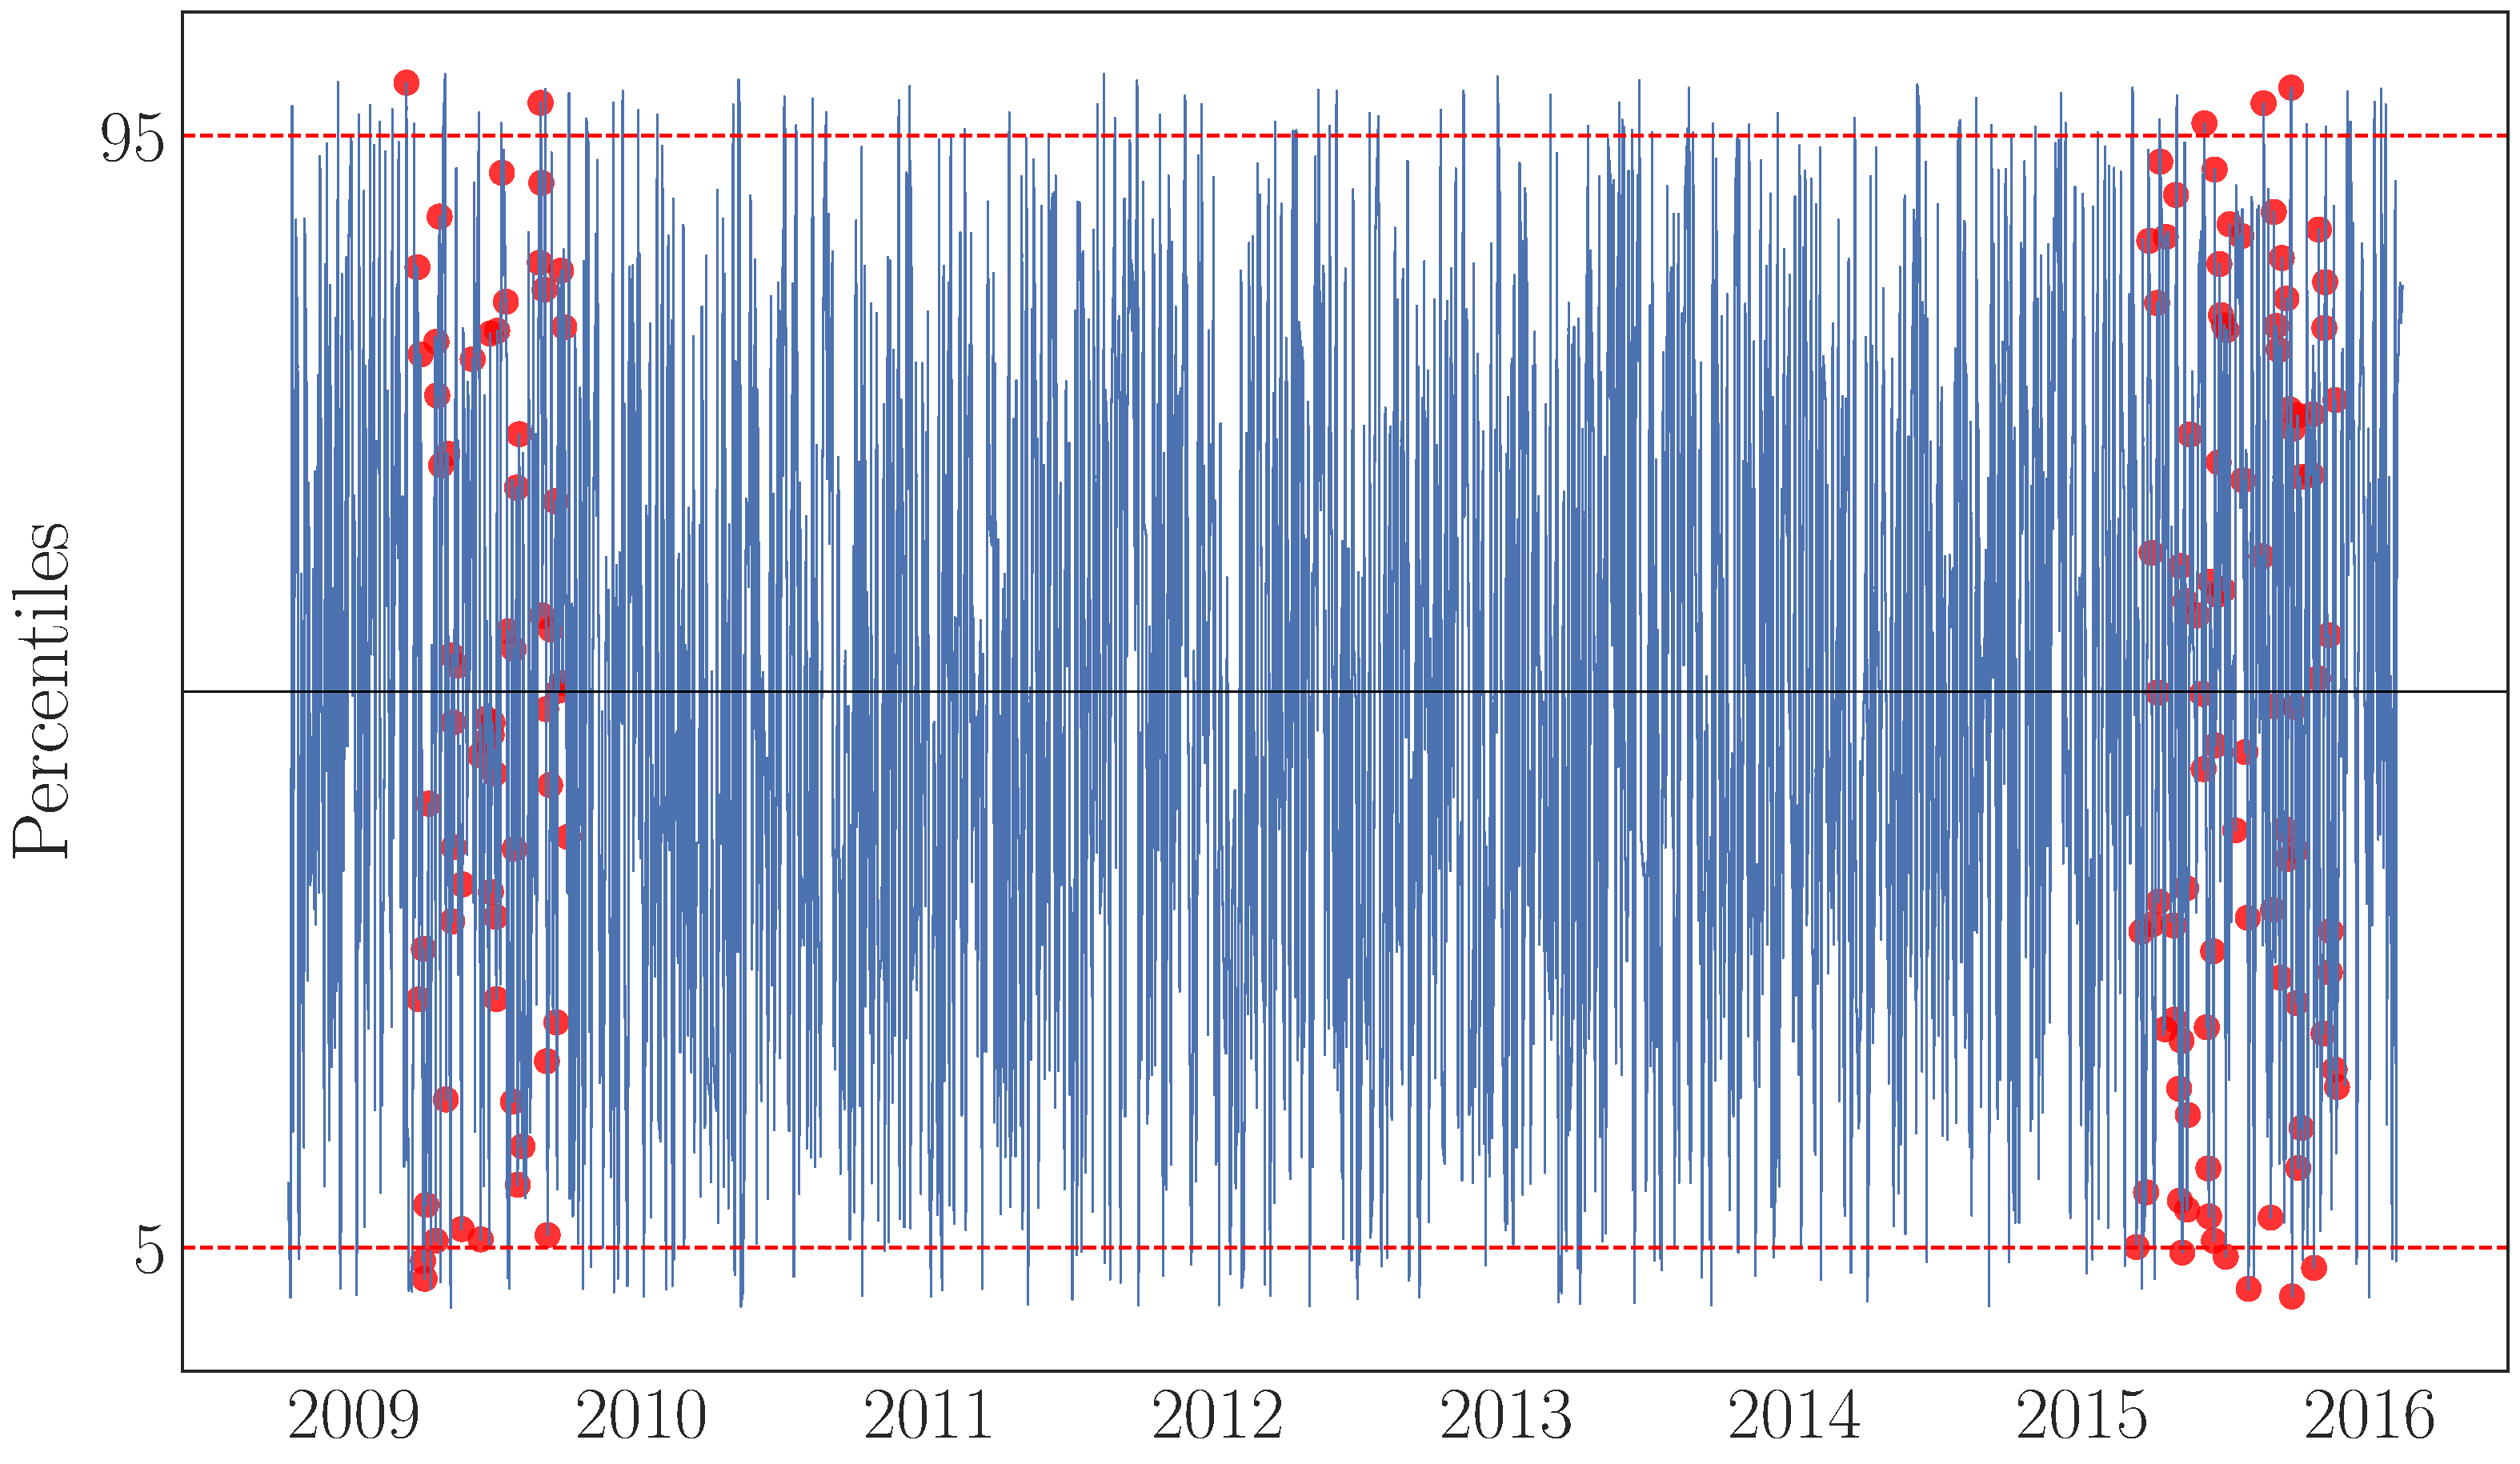
\includegraphics[width= 0.95\textwidth, keepaspectratio]{../output/benchmark_no_minprice_cdf.pdf}
\label{fig:benchmark-nominprice-cdf}
\source{\emph{Sources}: Banco Mexico and authors' calculations}
\end{figure}

%% ---------------------------------------------------------------------------
%% Conclusion
%% ---------------------------------------------------------------------------
\section{Conclusion}
\label{sec:conclusion}

FX  interventions  in  the  foreign  exchange  market  would  benefit  from  a
risk-based  approach. Central  banks use  quantitative  tools such  as VaR  to
measure the  risk they are taking  when they invest their  foreign reserves or
accept assets  as collateral  for their  loans. In this  paper, we  argue that
central banks could also  use this tool when they intervene  to support the FX
market, as intervention is tantamount to removing some exchange rate risk from
the market. A risk-based approach has very convincing advantages compared with
other types  of rules,  such as fixed-volatility,  or interventions  without a
minimum  price, because  it allows  the central  bank to  control exactly  the
exchange rate risk to which the economy  is exposed. It adds also the benefits
of being budget  neutral over the medium term, forward  looking, and combining
several market indicators into one.\\

The  back-testing  based  on  Mexico  data  is  supportive  of  rule-based  FX
intervention,  as  far as  the  risk  dimension  is concerned.  Our  framework
suggests that  fixed rules are broadly  consistent with a high  risk level. On
the contrary,  interventions without a  minimum price  appear to be  driven by
other rationales than exchange rate volatility and risk.\\

No central  bank is  currently known  to use  the VaR  rule, because  it comes
across as  difficult to communicate  or because policymakers prefer  to remain
discrete about  the intervention  decision. We  argue that  transparency could
help to  alleviate communication  challenges because  VarR-based interventions
provide  objective  and simple  triggers  in  terms  of a  bilateral  exchange
rate. However,  our VaR  rule should  be part of  a broader  communication and
operationalization strategy of the central bank in order to guarantee a smooth
and efficient implementation.\\

While policymakers are entitled to maintain full discretion over policymaking,
the paper  argues that  using VaR  as an  input would  contribute to  a better
informed decision, by anchoring the decision to intervene based on policymaker
risk tolerance and structural weaknesses of the economy, for example, unhedged
exposures. In summary, the VaR rule, while not currently widely used, could be
considered as one option to improve the rules that central banks use.\\

The model  of this paper  may have several  policy implications. The  VaR rule
would  be particularly  helpful for  central banks  concerned about  financial
stability risk  arising from the  exchange rate,  but committed to  a floating
exchange rate  arrangement in the  context of an inflation  targeting monetary
policy framework. The central banks could accompany the transition to exchange
rate flexibility by formalizing  the commitment to the float in  a rule and by
gradually   adapting   interventions  to   allow   for   more  exchange   rate
volatility. Finally, the  VaR rule could be used to  foster the development of
hedging markets by keeping a fixed amount  of risk in the market (usually most
of it) while absorbing some.\\

Looking beyond interventions in the spot  FX market, the same model and method
can be used  to measure the risk  transfers from any markets  that the central
banks  deem  useful  to  intervene  in  to  support  financial  stability.  In
particular, VaR models  can be used to  measure risk based on  spreads such as
(1) between actual and theoretical forward rates for the exchange rate hedging
market;  (2) between  onshore and  offshore USD  interest rates  for local  FX
funding  market; and  (3)  between risky  and risk-free  rates  for the  local
currency-denominated fixed income market.\\

One issue that remains to be addressed  is how to determine the risk tolerance
in VaR. The paper quotes the factors  underpinning it in broad terms, that is,
direct and indirect  exposures to exchange rate risk. However,  it is, so far,
left to the  policymakers' judgment to translate those  vulnerabilities into a
risk tolerance level (a target VaR). A method that estimates the extent of the
vulnerabilities  and  combined  them  with  their  impacts  on  macrofinancial
stability would be most useful.\\


%% ---------------------------------------------------------------------------
%% Bibliography
%% ---------------------------------------------------------------------------
\newpage
\addcontentsline{toc}{section}{References}
\singlespacing
\bibliographystyle{apalike2}
\bibliography{bibliography}

%% ---------------------------------------------------------------------------
%% Annex I
%% ---------------------------------------------------------------------------
\newpage
\appendix 
\section{Comparative Static Financial Performances}
\label{sec:fin-perf}

This  appendix  presents a  comparative  static  evaluation of  the  financial
performance of  the three  different intervention  strategies studied  in this
paper: the strategy without a minimum price, the strategy with a minimum price
(rule-based), and  the VaR  rule strategy.  We selected  a one-year  period of
intervention,  between  October  2015  and  October  2016.  The  frequency  of
intervention  under the  no minimum  price  and the  minimum price  strategies
during this  time was the same  (18 interventions each), with  similar volumes
(USD 3.32 billion  and USD 3.6 billion, respectively). Then,  we constructed a
series of  interventions following  the VaR  rule at  a similar  frequency (18
interventions), corresponding to a 10  percent intervention threshold, only on
the selling side to match the other strategies. We calibrated the intervention
amount  of the  VaR rule  to be  at  the average  under the  no minimum  price
strategy so that  the total amount of intervention under  the VaR rule exactly
matched the intervention amount under the no minimum price strategy.\\

This financial benchmarking is purely a comparative exercise. It might be that
some interventions without  a minimum price complemented  interventions with a
minimum price  and were executed at  a less favorable time.  The comparison is
not taking such a selection effect  into account and should not be interpreted
as  definite  proof of  the  financial  performance  of one  strategy  against
another.  Under  this  caveat,  the benchmarking  shows  that  the  rule-based
strategies (either  minimum price or  VaR based) outperform the  minimum price
strategy, as presented in the table below.\\

Table \ref{tab:financial-perf} reports  that on average, under  the no minimum
price  rule, the  central bank  was selling  USD when  the local  currency was
slightly appreciating against  the USD (by -6 bps; the  negative value in this
quotation  means appreciation).   Under the  minimum  price and  the VaR  rule
schemes,  on the  contrary, the  central bank  was selling  USD during  a more
favorable time.  By design, the VaR  rule is selecting days  with particularly
large depreciation, in  the order of 160 bps. Likewise,  the minimum price and
VaR rule scheme were  executed at much better rates in  terms of level.  While
the VaR rule  is designed to target the tails  of the conditional distribution
of the  log returns, it does  not necessarily guarantee that  the intervention
will happen  at the most favorable  exchange rate level. Our  simulation shows
that on average, it does nevertheless trigger interventions under better terms
than for the two other schemes.\\

Looking  at the  performance against  the  strategy without  a minimum  price,
computed against  the gain realized by  selling on average the  same volume of
USD at different points in time,  the benchmarking exercise indicates that the
minimum price  intervention would  outperform the  strategy without  a minimum
price by 7 percent, while the VaR rule would outperform it by 8.3 percent.\\

\begin{table}
  \begin{center}
    \caption{Financial Performances with and without Minimum Price}
%\footnotesize  %%  command to change the font size
\begin{tabular}{llll}
\toprule
{} & No minimum price & Minimum price & VaR rule \\
\midrule
Daily variation bps                  &             -6.1 &         108.8 &    164.8 \\
Average exchange rate                &             16.6 &          17.8 &       18 \\
FX Performance against discretionary &              0 \% &         6.9 \% &    8.3 \% \\
Total volume bn USD                  &             3.32 &           3.6 &     3.32 \\
Number of interventions              &               18 &            18 &       18 \\
\bottomrule
\end{tabular}

%\normalsize
\source{\emph{Sources}: authors’ calculations}
\label{tab:financial-perf}
\end{center}
\end{table}

\clearpage

%% ---------------------------------------------------------------------------
%% Annex II
%% ---------------------------------------------------------------------------
\section{Out-of-Sample Benchmarking}
\label{sec:benchmarking}

This  appendix  presents  a  series  of alternative  models  to  estimate  the
conditional density of  foreign exchange log returns over  time.  Our baseline
model  relies on  an EGARCH(1,1)  with a  Tskew parametrization  of the  error
terms’ distribution.   The conditional benchmark  models use the same  sets of
variables as our baseline model, presented in Section \ref{sec:specification},
and the same training/testing set.\\

We conduct benchmarking against:

\begin{itemize}
\item Different parametric variations of the GARCH model
  \begin{itemize}
  \item EGARCH(1,1) with Gaussian errors
  \item GARCH(1,1) with Tskew
  \item GARCH(1,1) with Gaussian errors
  \end{itemize}
\item Density estimation via quantile regressions. The full-fledged density is
  obtained via quantile interpolation and resampling, following the
  rearrangement procedure of \cite{chernozhukov2010}.
\item Unconditional distribution, estimated via Gaussian KDE on historical data
\end{itemize}

We assess  the performance metrics  of these models out-of-sample  against our
baseline model using (1)  PIT tests and (2) a density  log score, as explained
in \cite{diks2011}; we use the uncensored version of the log score.\\

We summarize  the results in  Table \ref{tab:benchmark-perf}. We  define "pass
the PIT  test" as: if  the estimated invert  CDF distribution lies  within the
uniform distribution  +/- 5 percent  interval confidence bands, as  defined in
\cite{rossi2019}, and "fail"  otherwise.  Regarding the density  log score, we
provide  both the  test statistic  (the average  difference of  the log  score
across  time)  and  the  p-value  of  the  test  statistic,  as  explained  in
\cite{diks2011}.   A   positive  test  statistic  indicates   that  the  model
outperforms the baseline  model, while the p-value tested  the null hypothesis
that the log scores of the two models are the same.\\

\begin{table}
  \begin{center}
    \caption{Results of the Out-of-Sample Benchmark Tests}
%\footnotesize  %%  command to change the font size
\begin{tabular}{lccc}
\toprule
  & PIT & Logscore diff against Baseline & Diff pvalue \\ 
  \midrule
	Baseline & Pass &  &  \\ 
	Unconditional & Fail & -6.36 & 0 \\ 
	Quantile Reg & Pass & -2.09 & 0.02 \\ 
	Gaussian EGARCH & Fail & 1.235 & 0.892 \\ 
	TSkew GARCH & Fail & 1.536 & 0.937 \\ 
  Gaussian GARCH & Fail & 1.86 & 0.968 \\ 
\bottomrule
\end{tabular}

%\normalsize
\source{\emph{Sources}: authors’ calculations}
\label{tab:benchmark-perf}
\end{center}
\end{table}

As Table \ref{tab:benchmark-perf} shows, the baseline model has a better log score than the
unconditional distribution and the daily distribution fitted from the quantile
regressions model  with resampling,  and these  two models  both fail  the PIT
test. However,  the difference against  variation of  the GARCH model  is less
clear cut:  while the  other models  outperform the baseline  in terms  of log
score,  the difference  is not  significant and  they also  fail the  PIT test
(albeit only  by a very  few numbers of  percentiles). Therefore, while  it is
clear that the GARCH specification is  appropriate to model FX returns―in line
with  the  literature―variations   around  the  type  of   GARCH  and  implied
distributions are statistically equivalent.\\

\begin{figure}
  \centering
  \caption{Unconditional Distribution PIT Test, Out-of-Sample}
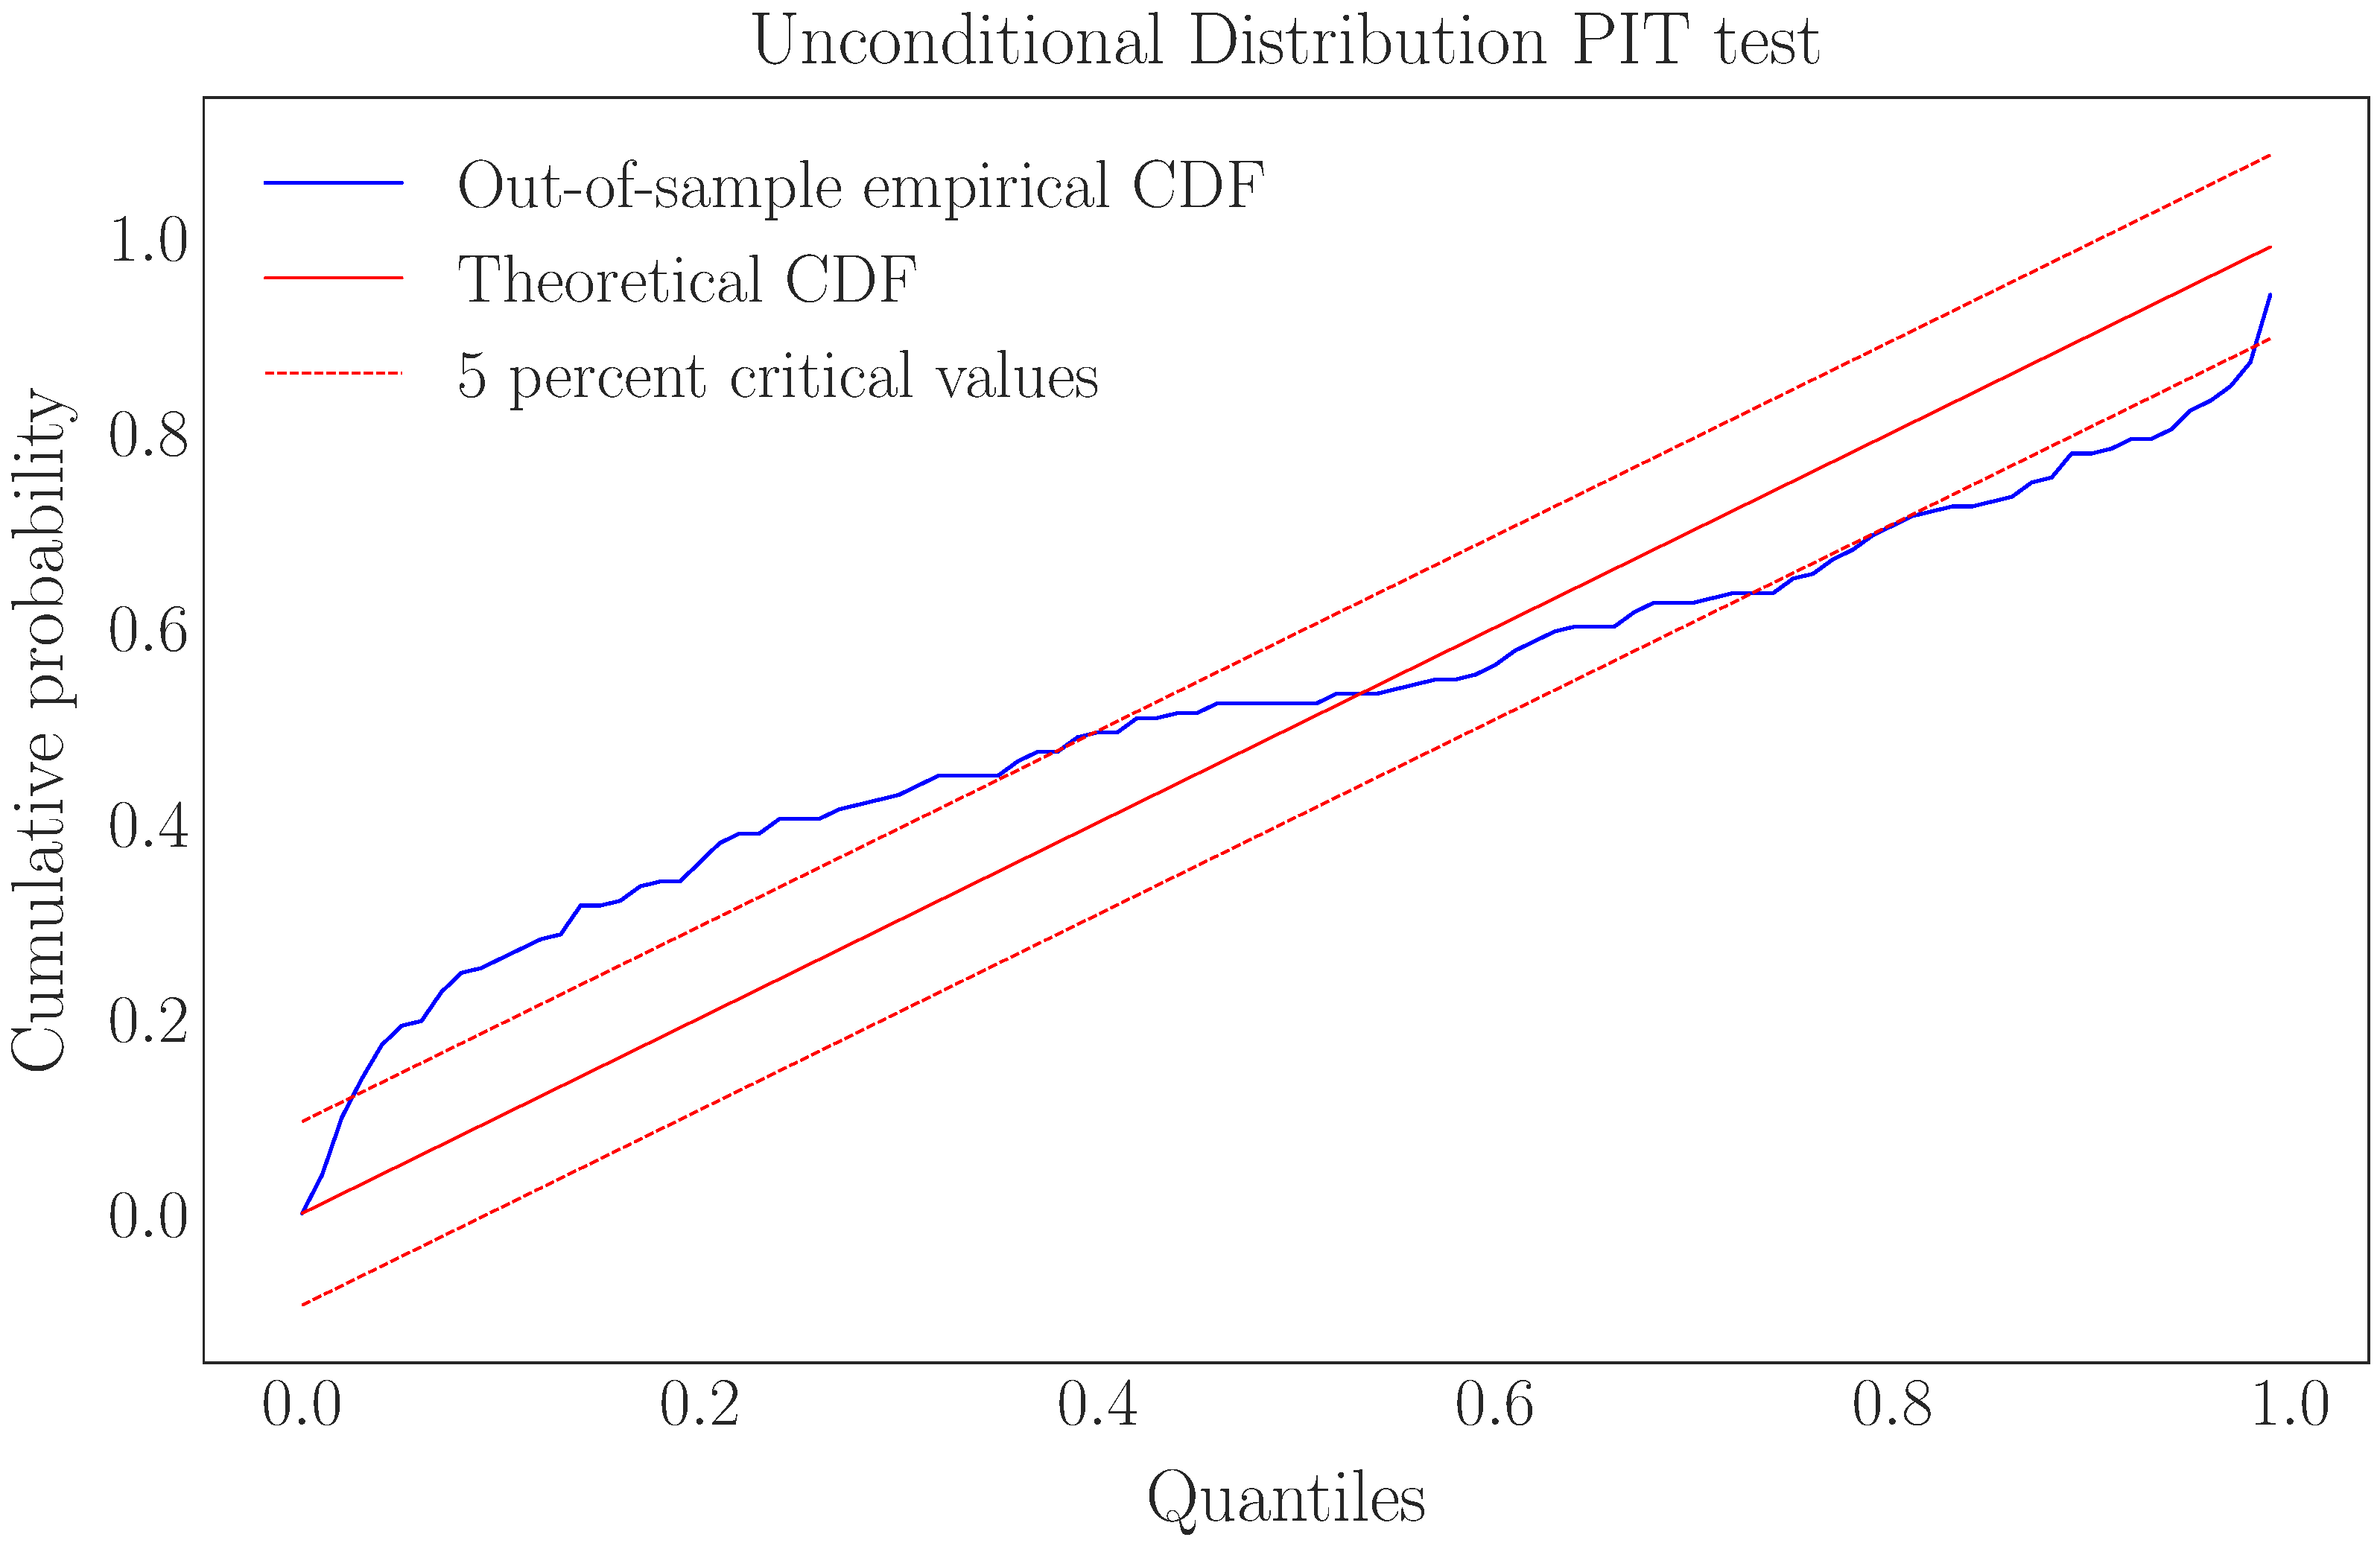
\includegraphics[width= 0.95\textwidth, keepaspectratio]{../output/pit_chart_unconditional.pdf}
\label{fig:pit-chart-unconditional}
\source{\emph{Sources}: authors' calculations}
\end{figure}

\begin{figure}
  \centering
  \caption{Quantile Regression Distribution PIT Test, Out-of-Sample}
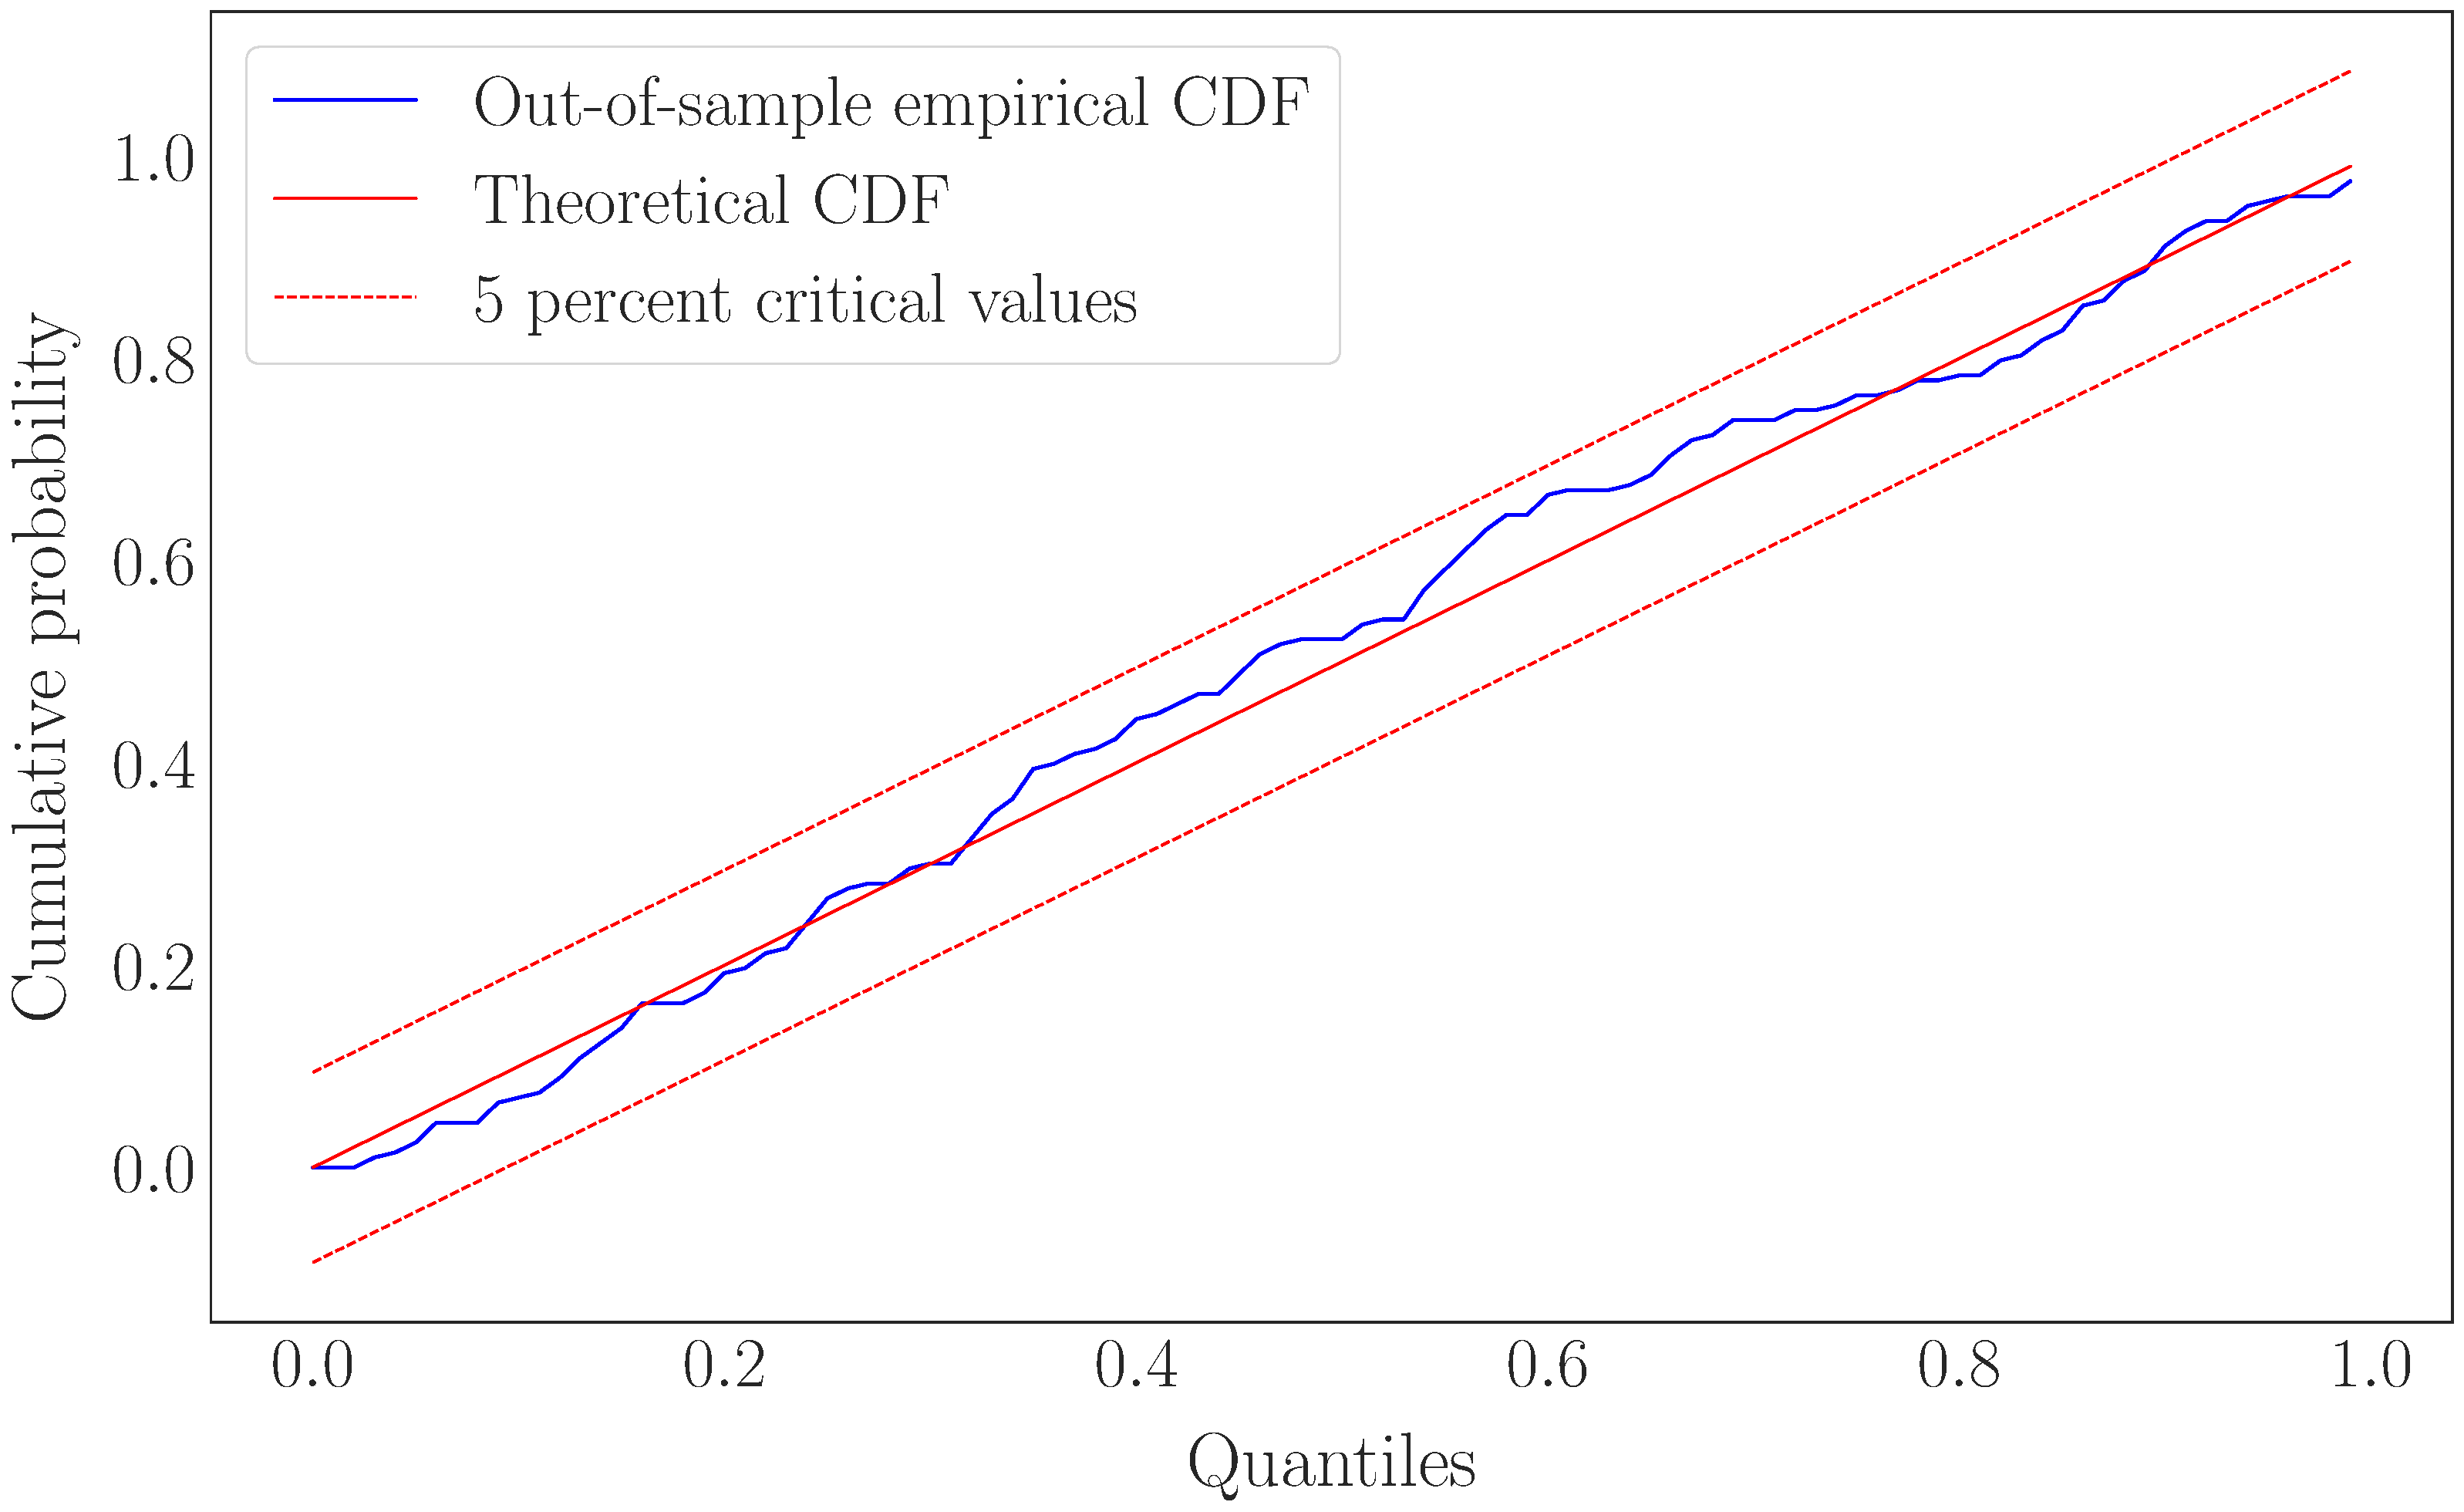
\includegraphics[width= 0.95\textwidth, keepaspectratio]{../output/pit_chart_qreg.pdf}
\label{fig:pit-chart-qreg}
\source{\emph{Sources}: authors' calculations}
\end{figure}


\begin{figure}
  \centering
  \caption{GARCH TSkew Benchmark PIT Test, Out-of-Sample}
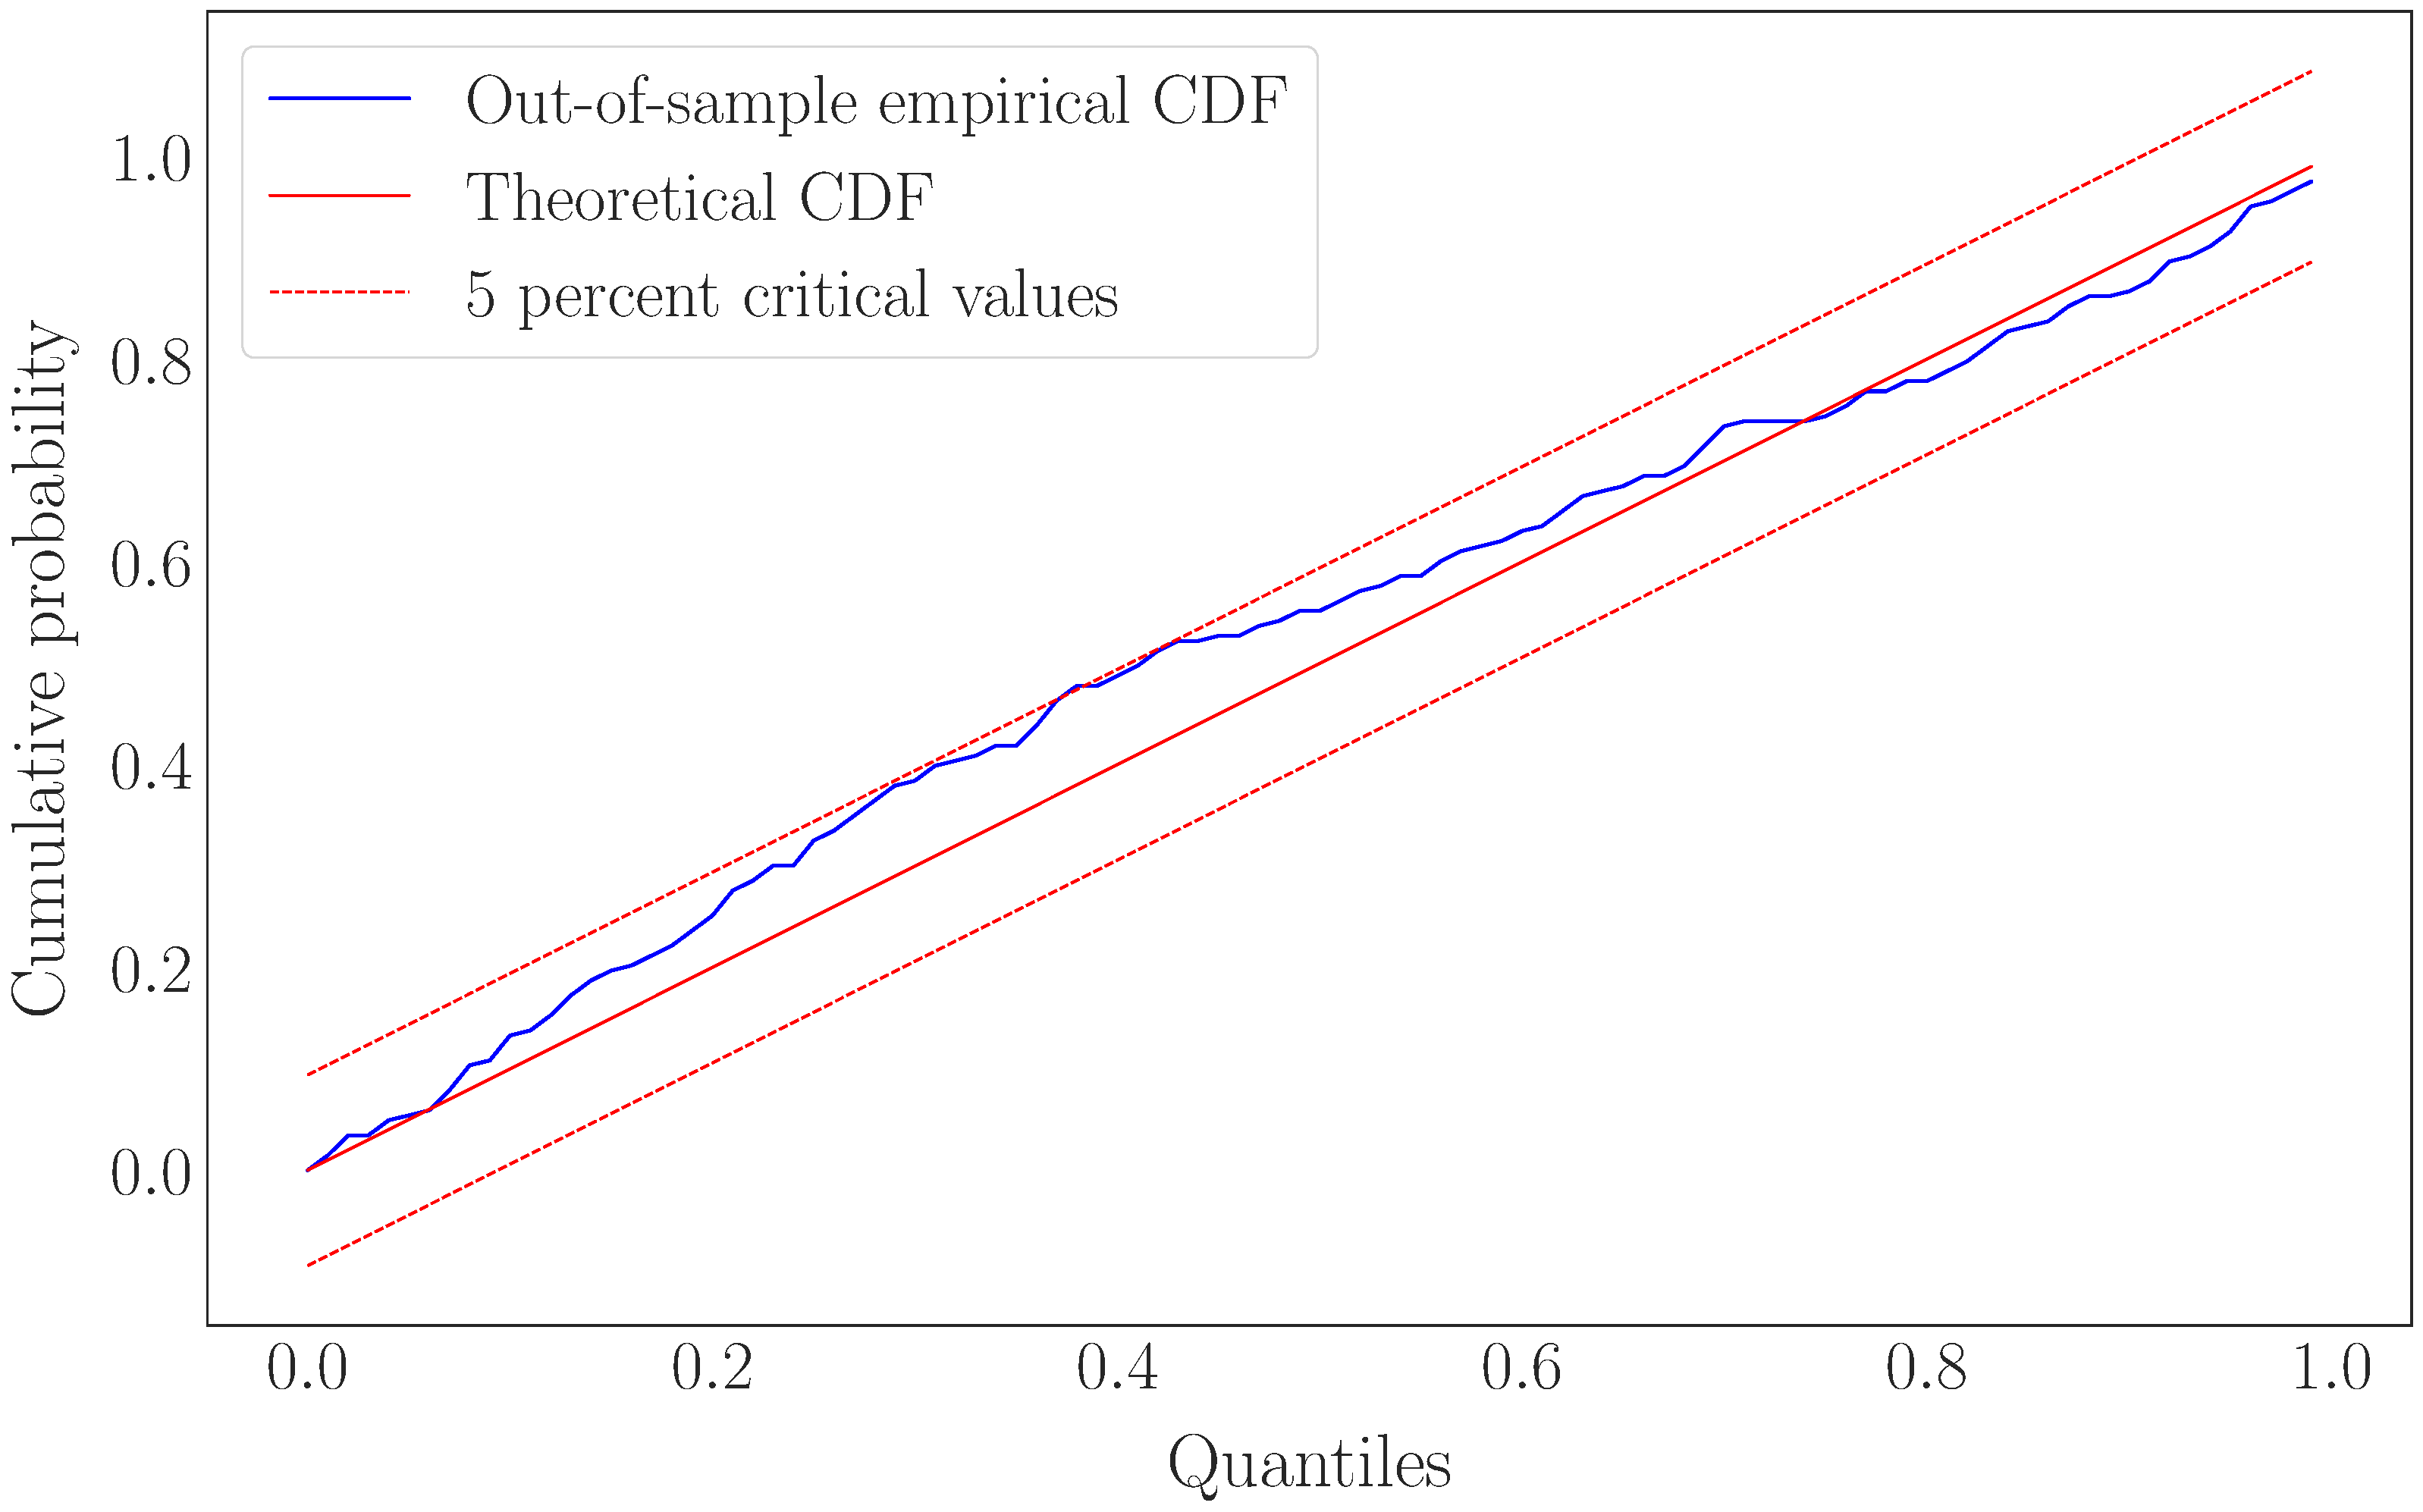
\includegraphics[width= 0.95\textwidth, keepaspectratio]{../output/pitchart_garch_tskew.pdf}
\label{fig:pit-chart-qreg}
\source{\emph{Sources}: authors' calculations}
\end{figure}







%% ---------------------------------------------------------------------------
%% End the document
%% ---------------------------------------------------------------------------
\end{document}
